%% This document gives an example on how to use the ntnumasterthesis
%% LaTeX document class.

%% Use short name MACS, MIS, CIMET, MTDMT, MIXD or MIS  
%% Language english or norsk
%% b5paper with oneside or twoside, you can set A4 if you want but you submit in b5

%% If you want print with the heading material on a4 paper you can use this format
%% \documentclass[MACS,en glish,a4paper,oneside,12pt]{ntnuthesis/ntnuthesis}

%% with the change to using DAIM we have a new option. include DAIM after english below removes the front page material so that you can then submit in the DAIM system. If you are wanting the front material remove DAIM and make sure you fill in the DaimData.tex file.
\documentclass{report}
%[MACS,english]{ntnuthesis/ntnuthesis

\usepackage[T1]{fontenc}
\usepackage[utf8]{inputenc}     % For utf8 encoded .tex files allows norwegian characters in the files. This can be dangerous if you change to a differnt editor.
%\usepackage[pdftex]{graphicx, hyperref}   % For cross references in pdf
\usepackage{graphicx}
\usepackage{hyperref}   % For cross references in pdf

% For smart references 
%    use \cref{label} and Caption and Number will be added automatically
\usepackage[capitalise,noabbrev]{cleveref} 
\usepackage[nottoc]{tocbibind}
\usepackage{url}
\usepackage{color}              % For colouring text 
\hypersetup{colorlinks=true,     
		linkcolor=black,          % color of internal links (change box color with linkbordercolor)
    citecolor=black,        % color of links to bibliography
    filecolor=black,      % color of file links
    urlcolor=black           % color of external links
		}
\usepackage{csvsimple}  % for simple table reading and display
\usepackage{url}
\usepackage{booktabs}
\usepackage{gnuplottex} %miktex option if using miktex on windows
\usepackage{rotating}
\usepackage{gensymb}
\usepackage{float}
\usepackage[utf8]{inputenc}
\usepackage{enumitem}
\usepackage{multirow}
\usepackage{amssymb}
\usepackage{amsmath}
\usepackage{tocloft}
\usepackage{float}
\usepackage{appendix}
\renewcommand*\contentsname{Contents}
\usepackage{array}
\usepackage{subfig}
\usepackage{color}
\usepackage{gensymb}
\usepackage{multicol}
\usepackage{listings}
\usepackage{varwidth}
\usepackage{enumitem}
\usepackage{chngcntr}
\usepackage{fancyhdr}
\counterwithin{figure}{section}
\usepackage{vmargin}
\usepackage{datetime}
\usepackage{pdfpages} 
\usepackage{adjustbox}
\usepackage{rotating}
\usepackage{ctable}
\usepackage[toc,page]{appendix}
%\usepackage{fourier}
\setlength\parindent{0pt}
\usepackage{units}
\usepackage{wrapfig}

\pagenumbering{roman}

\setmarginsrb{3 cm}{2.5 cm}{3 cm}{2.5 cm}{1 cm}{1.5 cm}{1 cm}{1.5 cm}
\pagestyle{fancy}
\fancyhf{}
\rhead{\theauthor}
\lhead{\thetitle}
\cfoot{\thepage}


\pagestyle{fancy}
\fancyhf{}
\rhead{\theauthor}
\lhead{\thetitle}
\cfoot{\thepage}
\title{Fatigue of Dynamic Power Cables Applied in Offshore Wind Farms}								% Title
\author{Karoline Bakken}								% Author
\date{Spring 2019}											% Date

\makeatletter
\let\thetitle\@title
\let\theauthor\@author
\let\thedate\@date
\makeatother


\definecolor{darkgreen}{rgb}{0,0.5,0}
\definecolor{darkred}{rgb}{0.5,0.0,0}

\lstset{        basicstyle=\ttfamily,
                keywordstyle=\color{blue}\ttfamily,
                stringstyle=\color{darkred}\ttfamily,
                commentstyle=\color{darkgreen}\ttfamily,
}

\usepackage{vmargin}
\setmarginsrb{3 cm}{2.5 cm}{3 cm}{2.5 cm}{1 cm}{1.5 cm}{1 cm}{1.5 cm}

%Typesetting of C++ but not always stable in titles etc...
\newcommand{\CPP}[0]{{C\nolinebreak[4]\hspace{-.1em}\raisebox{.1ex}{\small\bf +\hspace{-.1em}+\ }}}

%\usepackage[table]{xcolor}% http://ctan.org/pkg/xcolor
%\usepackage[nomessages]{fp}
%\newlength{\maxbarlen}


\newcommand\databar[3][gray!20]{%
  \FPeval\result{round(#3/#2:4)}%
  \rlap{\textcolor{#1}{\hspace*{\dimexpr-\tabcolsep+.5\arrayrulewidth}%
        \rule[-.05\ht\strutbox]{\result\maxbarlen}{.95\ht\strutbox}}}%
  \makebox[\dimexpr\maxbarlen-2\tabcolsep+\arrayrulewidth][r]{#3}}



\newcommand{\com}[1]{{\color{red}#1}} % supervisor comment
%\renewcommand{\com}[1]{} %remove starting % to remove supervisor comments
% This will appear in text \com{Lecuters comment} and be visible unless you uncomment
% the renewcommand line.

\newcommand{\todo}[1]{{\color{green}#1}} % items to do
%\renewcommand{\todo}[1]{} %remove starting % to remove items to do

\newcommand{\n}[1]{{\color{black}#1}} % other comment
%\renewcommand{\n}[1]{} %remove starting % to remove notes

\newcommand{\dn}[1]{} % add the d to a note to say that you have finished with it.





% Set to true ONLY if using Harvard citation style
\newboolean{HarvardCitations}
\setboolean{HarvardCitations}{true} % false for computer science, true for interaction design and harvard style


\ifthenelse{\boolean{HarvardCitations}}{%
	\usepackage{natbib} % for Harvard names as citations.
}{%
	\usepackage[numbers]{natbib} % for Vancover numbers in bibliography
}

%\newcommand{\q}[1]{\leavevmode\marginpar{\small\em #1}}
%\renewcommand{\q}[1]{}


\usepackage{nomencl}
\makenomenclature
 
%% This code creates the groups
% -----------------------------------------
\usepackage{etoolbox}
\renewcommand\nomgroup[1]{%
  \item[\bfseries
  \ifstrequal{#1}{RL}{Roman Letters}{%
  \ifstrequal{#1}{MV}{Matrices and Vectors}{%
    \ifstrequal{#1}{GL}{Greek Letters}{%
  \ifstrequal{#1}{AB}{Abbrevations}{}}}}%
  
]}

\begin{document}

\begin{titlepage}
	\centering
    \vspace*{0.5 cm}
    
\includegraphics[scale = 0.3]{figures/ntnuu}\\[1.0 cm]	% University Logo
    \textsc{\LARGE Norwegian University of Science \newline\newline and Technology}\\[2.0 cm]	% University Name
	%\textsc{\Large Karoline Bakken}\\[0.5 cm]				% Course Code
	\rule{\linewidth}{0.2 mm} \\[0.4 cm]
	{\huge \bfseries \thetitle}\\
	\rule{\linewidth}{0.2 mm} \\[1.5 cm]
	
	\textsc{\Large Karoline Bakken}\\[0.5 cm]
	\Large{June 2019}\\[1.5 cm]
	Master Thesis\\
	Department of Marine Technology \\
	Norwegian University of Science and Technology
	\vfill
		\begin{flushleft} Supervisor: Professor Svein Sævik
		\end{flushleft}
	 
	 
	 
	 \begin{comment}
	 
	
	\begin{minipage}{0.4\textwidth}
		\begin{flushleft} \large
			\emph{Supervisor:}\\
			Professor Svein Sævik
			\end{flushleft}
			\end{minipage}~
			\begin{minipage}{0.4\textwidth}
            
			\begin{flushright} \large
			\emph{Author:} \\
			Karoline Bakken
		\end{flushright}
        
	\end{minipage}\\[2 cm]
	
	 \end{comment}
    
    
    
    
	
\end{titlepage}
\clearpage\mbox{}\clearpage
%% for students submitting in the DAIM system this information will not be used.
% their is an option for DAIM submission which removes this information and checks it is B5.
% Removing the DAIM option on the document type will use this material.

%\setthesistitle{Project Thesis. Fatigue of Dynamic Power Cables applied in Offshore Wind Farms}
%\setthesisshorttitle{Example Masters Thesis} % a short version for the page headers if your normal title is too long to fit
%\setthesisauthor{Karoline Bakken}
%\setthesissupervisor{Prof. Svein Sævik}
%\setthesissupervisorA{Prof. Jon Yngve Hardeberg}  % if you have a second supervisor add it like this
%\setthesissupervisorB{Prof. Smart Guy}  % if you have a second supervisor add it like this


%\nmtkeywords{Thesis, Latex, Template, IMT}
%\nmtdesc{This is the short description of a masters thesis}


%\setthesisdate{01-06-2017}
%\setthesisyear{2017}



%for CIMET theses you need to see all of these as well

%\setthesiscampus{Gj\o{}vik}
%\setthesisHostInstitution{\NTNU}
%\setthesisHostInstitution{University of Eastern Finland}
%\setthesisHostInstitution{Universit\'e Jean Monnet Saint-Etienne}

%\setthesisjuryA{} %jury names
%\setthesisjuryB{} %jury names
%\setthesisjuryC{} %jury names
%\setthesisjuryD{} %jury names


 % this is the file which contains all the details about your thesis
%\makefrontpages % make the frontpages
%\input{inc/mastersIntro}
%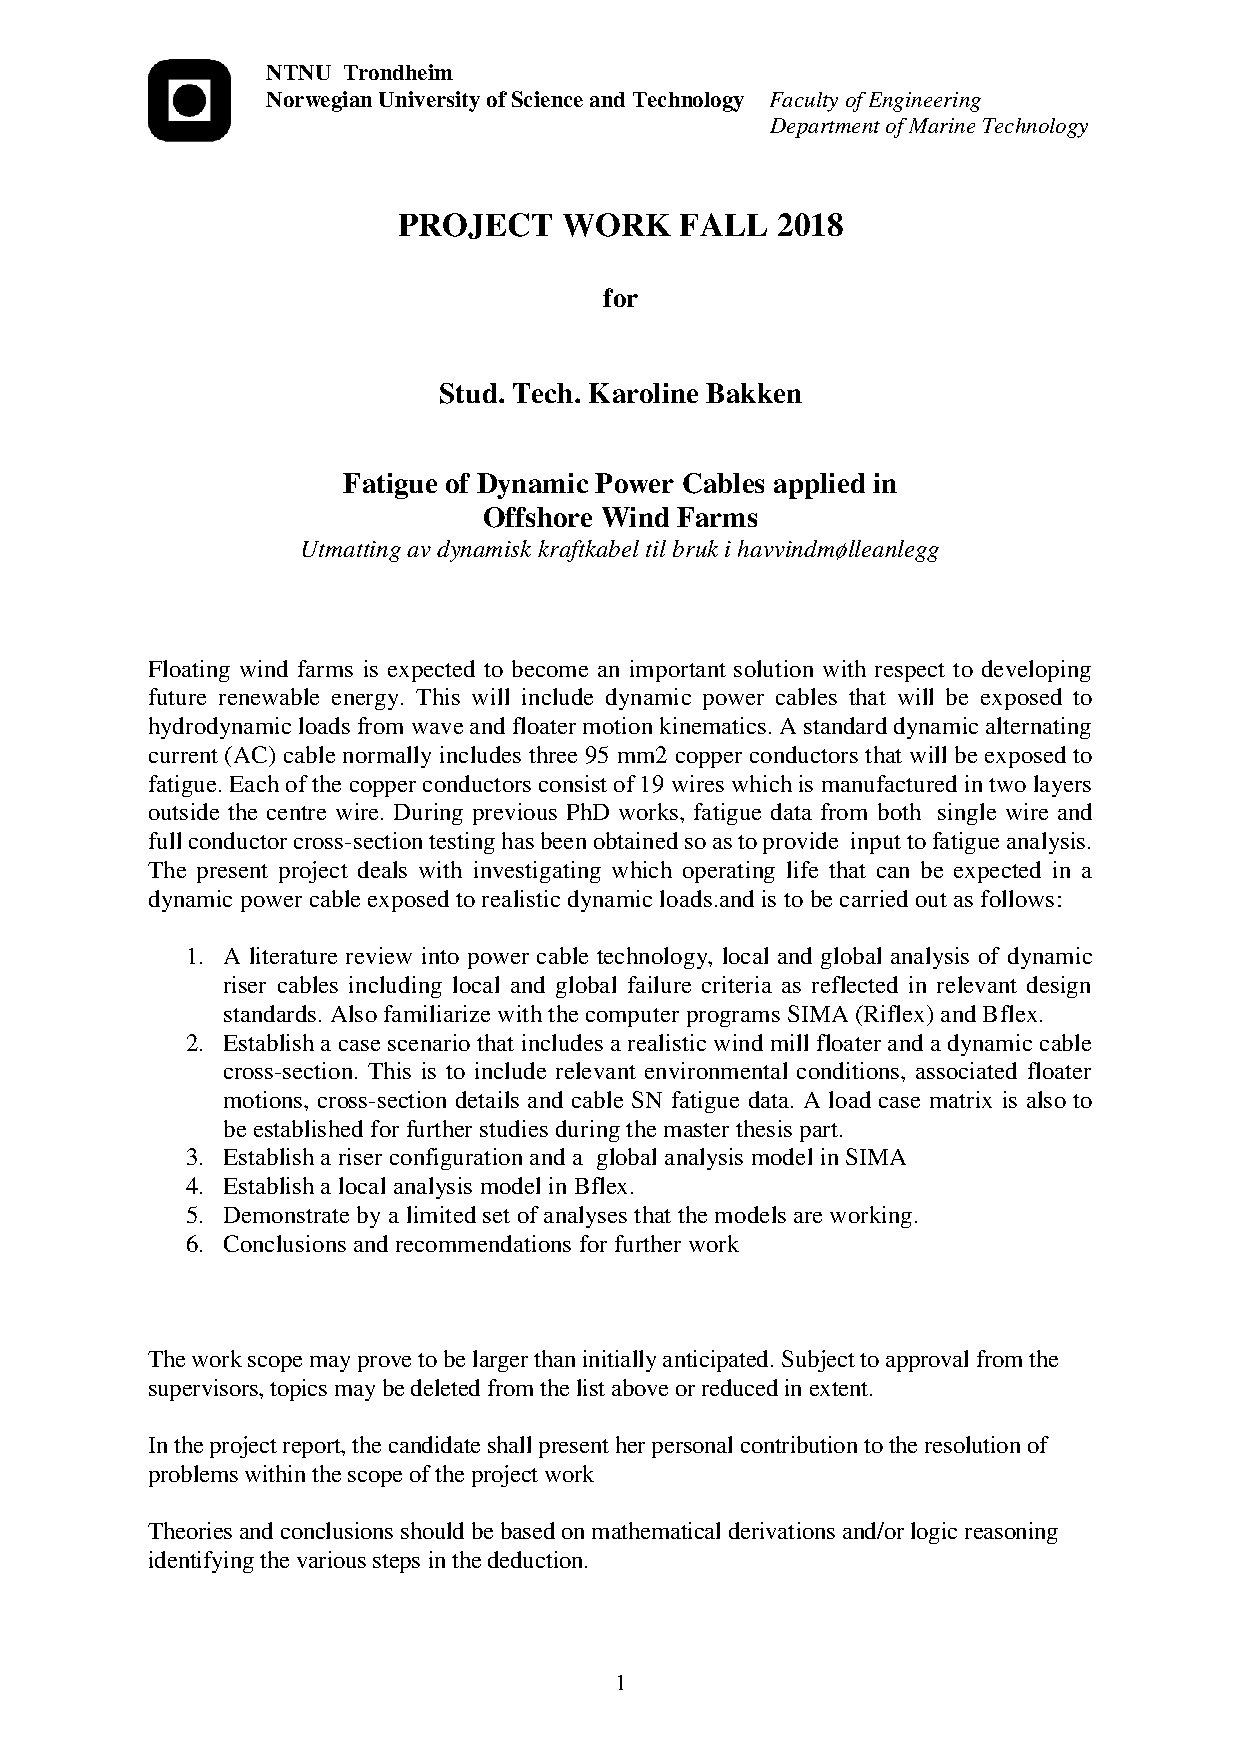
\includepdf[pages=-]{inc/description} 
\setboolean{@twoside}{false}
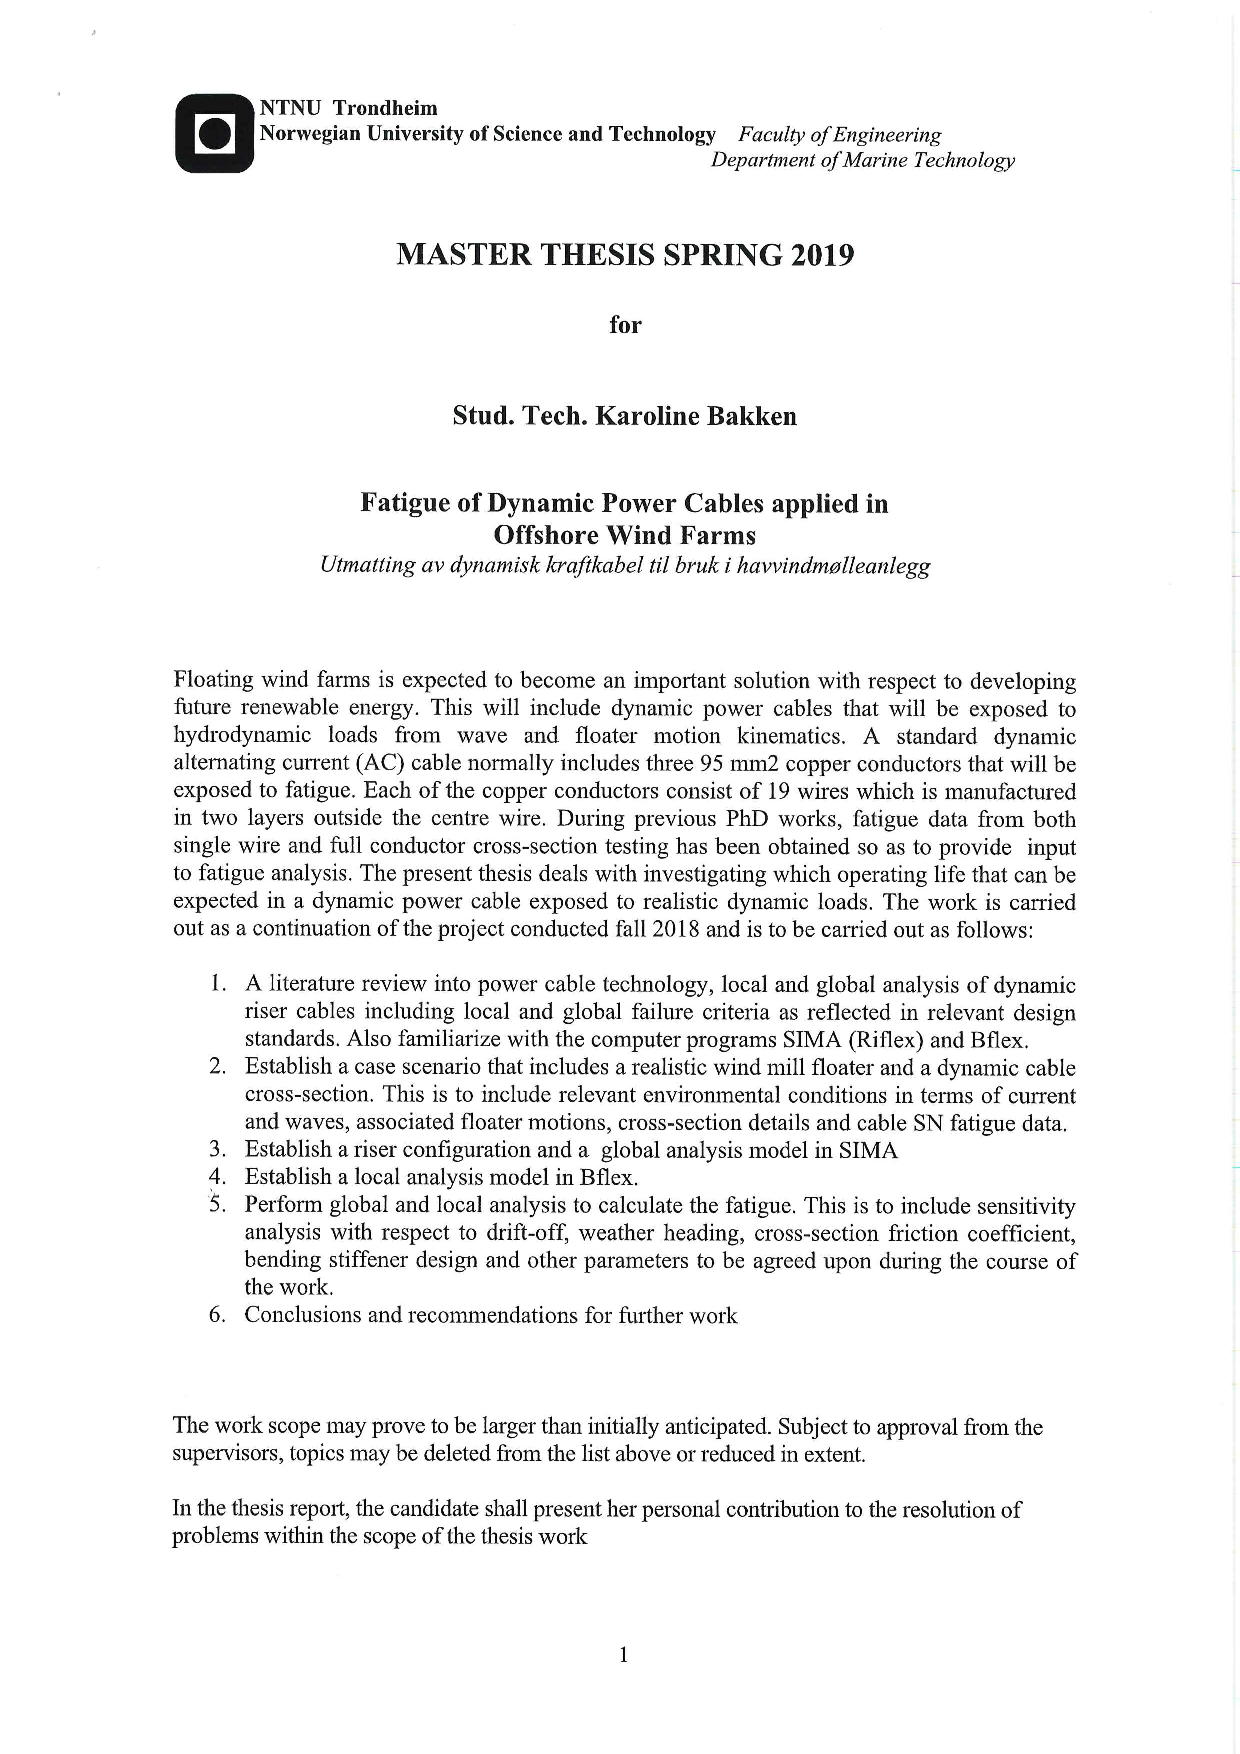
\includepdf[pages=-, offset=75 -75]{inc/masteravtale.pdf}
%\thesistitlepage % make the ordinary titlepage
\hypersetup{pageanchor=true}
%\chapter*{Abstract}

As offshore wind energy installations are moving into deeper waters, and further away from shore, floating wind installations are necessary. The dynamic power cable that will deliver the electricity from the installation is an important component for this technology. There has been a lot of research on the fatigue life on dynamic slender structures in the oil and gas industry, but very little in dynamic power cables applied in offshore wind. Learning more on fatigue of power cables is a key component in order to advance in offshore floating wind technology. Generally, a power cable consists of conductors with an assembly of wires helically stranded in layers around a core, causing contact between layers as well as between layers. This adds a vulnerability for fretting fatigue to the cable. This was investigated further by performing a global and a local analysis. The floating wind turbine OO-Star was chosen as a case study. This is a design done by Dr. Techn. Olav Olsen, and is participating in the project Lifes50+. West of Barra, Scotland was chosen as location, and the cable design was developed in close dialogue with Professor Svein Sævik. \\\\SIMA RIFLEX was used for the global model, where the whole cable was modelled with attachment to the sea floor, and a point behaving like the wind turbine floater due to given transfer functions provided by Dr. Techn. Olav Olsen. The configuration of the cables was based on no compression in the cable and a max curvature that could not be exceeded in the static or dynamic analysis for neither wind condition or position. As a simplification, three different wind conditions and positions were included.  The local model was created in BFLEX, and only the upper part of the cable was modelled as it was assumed that this is were the largest fatigue damage is located. The local model consisted of a stiff pipe, a bend stiffener and a cable with several layers. \newline 
\newline
The global analysis was performed by running each sea state in the scatter diagram for West of Barra for one hour each, and calculating the angle between the cable and vessel, and the tension in the upper element. Rainflow counting was used to count cycles in each angle class, and the classes were rearranged into 15 cases with angle range and corresponding tension. This was used as input in the local analysis were each angle and tension range were analyzed for one cycle. The curvature and tension in each case was used to calculate the stress range for each case in each layer of the conductor, and fatigue life was estimated by the use of an apropriate SN-curve.  \\\\
The fatigue life of the dynamic power cable was \todo{SKRIV INN ENDELIG FATIGUE LIFE}\\\
Also included in the Master Thesis are all the necessary theory necessary to execute the procedure described above. This includes theory about wind turbines, power cables, fatigue and the numeric theory behind the software used to create the two models. 


\chapter*{Preface}
 \newline
\newline
All the work have been executed by the author of the master thesis, Karoline Bakken. 
\newline
\newline
\newline
\newline
\newline
\newline
\begin{center}
    Trondheim, November 13th, 2018
    \end{center}
\begin{figure}[H]
\centering

\includegraphics[scale=0.5]{figures/sign}
\end{figure}
\begin{center}
Karoline Bakken
\end{center}
\chapter*{Acknowledgment}


\newline
\newline
\newline

\begin{flushright}
K.B.
\end{flushright}
\chapter*{Abstract}

As offshore wind energy installations are moving into deeper waters, and further away from shore, floating wind installations are necessary. The dynamic power cable that will deliver the electricity from the installation is an important component for this technology. There has been a lot of research on the fatigue life on dynamic slender structures in the oil and gas industry, but very little in dynamic power cables applied in offshore wind. Learning more on fatigue of power cables is a key component in order to advance in offshore floating wind technology. Generally, a power cable consists of conductors with an assembly of wires helically stranded in layers around a core, causing contact between layers as well as between layers. This adds a vulnerability for fretting fatigue to the cable. This was investigated further by performing a global and a local analysis. The floating wind turbine OO-Star was chosen as a case study. This is a design done by Dr. Techn. Olav Olsen, and is participating in the project Lifes50+. West of Barra, Scotland was chosen as location, and the cable design was developed in close dialogue with Professor Svein Sævik. \\\\SIMA RIFLEX was used for the global model, where the whole cable was modelled with attachment to the sea floor, and a point behaving like the wind turbine floater due to given transfer functions provided by Dr. Techn. Olav Olsen. The configuration of the cables was based on no compression in the cable and a max curvature that could not be exceeded in the static or dynamic analysis for neither wind condition or position. As a simplification, three different wind conditions and positions were included.  The local model was created in BFLEX, and only the upper part of the cable was modelled as it was assumed that this is were the largest fatigue damage is located. The local model consisted of a stiff pipe, a bend stiffener and a cable with several layers. \newline 
\newline
The global analysis was performed by running each sea state in the scatter diagram for West of Barra for one hour each, and calculating the angle between the cable and vessel, and the tension in the upper element. Rainflow counting was used to count cycles in each angle class, and the classes were rearranged into 15 cases with angle range and corresponding tension. This was used as input in the local analysis were each angle and tension range were analyzed for one cycle. The curvature and tension in each case was used to calculate the stress range for each case in each layer of the conductor, and fatigue life was estimated by the use of an apropriate SN-curve.  \\\\
The fatigue life of the dynamic power cable was \todo{SKRIV INN ENDELIG FATIGUE LIFE}\\\
Also included in the Master Thesis are all the necessary theory necessary to execute the procedure described above. This includes theory about wind turbines, power cables, fatigue and the numeric theory behind the software used to create the two models. 


\chapter*{Sammendrag}
Offshore wind energi installasjoner forflytter seg til dypere vann lenger unna kysten, noe som krever at insdtallasjonene er flytende. De dynamiske kraftkablene som veverer strlmmen fra installasjonene er viktige komponenter for denne typen teknologi. Mye forskning har blirr gjort på slake konstruksjoner i forbindelsemed olje og gass sindustrien, men svært lite er blitt gjort med tanke på utmatting i strøm kabler anvendt i flytende offshore wind teknologi. En strømkabel består vanligvis av ledere med en samling tråder som er orndet i spiraler rundt en kjærne. Dette skaper kontakt mellom både de forskjellige lederene, men også mellom lagene av tråder i hver leder, og gjør kablene sårbare for ulike utmattings mekanismer. \\\\
Dette temat ble undersøke nærmere ved å utføre både lokale og globale analyser. Den flytende vind turbinen OO-Star ble ansett som en interessant konstruksjon å bruke til dette prosjektet. OO-Star er et design som er utviklet av Dr. Techn. Olav Olsen som en del av forskningsprosjektet Lifes50+. West of Barra utenfor Skotland ble brukt som lokasjon, og kabeldesignet ble utformet i nøye dialog med Professor Svein Sævik. SIMA RIFLEX ble brukt i for å modellere den globale modellen som består av hele kabelen, festet til havbunnen og til et punkt på overflaten som beveger seg likt OO-Star gjennom transfer funksjonene gitt av Dr. Techn. Olav Olsen. Kabelkonfigurasjonen ble basert på kravet om ingen kompressjon i kabelen, samt en maks kuratur som ikke kunne overskrides. Kun tre vind tilstander med tilhørende flyterposisjoner ble brukt som en forenkling. Den lokale modellen bestod av den øvre delene av kabelen, ettersom det ble ansett som mest sannsynlig at utmattingsskadene ville være størst her. Den lokale modellen bestod av kabelen selv med dens mange lag, et stivt rør og en bøyestiver.\\\\
Den globale analysen be utført ved at alle sjøtilstandene beskrevet i scatter tabellen til West of Barra ble analysert i en time hver. Vinkelen mellom turbinkonstruksjonen og den øvre delen av kabelen ble regnet ut for hvert tidssteg, samt spenningen i det øverste elementet av kabelen. Rainflow counting ble brukt for å telle antall sykluser for hver vinkelklasse, som ble reorganisert inn til 15 klasser med vinkel og spenning for hver klasse. Dette ble brukt som input til den lokale analysen, der hver klasse  med vinkel og spenning ble analysert i en syklus. Den resulterende kurvaturen og spenningen for hver klasse ble brukt til å regne ut belastningsområdet for hver klasse og utmattigslevetiden ble regnet ut fra en passene SN-kurve. \\\\
Utmattingslevetiden til den dynamiske strømkabelen ble regnet ut til å være 641.28 år, og det ble konkludert med at det var stor effekt av frisksjon mellom lederene samt mellom lagene internt i hver leder. \\\\
Inkludert i denne masteroppgaven er også all nødvending teori for å utføre arbeidet beskrevet ovenfor. Dette inkluderer teori om vindturbiner, stømkabler utmatting og den numeriske teorien bak programmene som har blitt brukt for å modellere de to modellene. 
\tableofcontents

\hypersetup{pageanchor=true}

% Comment with a percent to remove figures or tables:
\listoffigures
\listoftables
%\lstlistoflistings
\begin{comment}
% -----------------------------------------
\nomenclature[P]{$c$}{Speed of light in a vacuum inertial system}
\nomenclature[P]{$h$}{Plank Constant}
\nomenclature[P]{$g$}{Gravitational Constant}
\nomenclature[N]{$\mathbb{R}$}{Real Numbers}
\nomenclature[N]{$\mathbb{C}$}{Complex Numbers}
\nomenclature[N]{$\mathbb{H}$}{Quaternions}
\nomenclature[O]{$V$}{Constant Volume}
\nomenclature[O]{$\rho$}{Friction Index}
 
\printnomenclature

\end{comment} 
\chapter*{Nomenclature}
\subsubsection*{Latin Letters}       
\begin{align*}
a    &\ \text{Acceleration}\\
A      &\ \text{Area, Amplitude}\\
A_1      &\ \text{Area before energy extraction}\\
A_2      &\ \text{Area after energy extraction}\\
b    &\ \text{Buoyancy}\\
c   &\ \text{Constant}\\
C_P      &\ \text{Power coefficient (Betz Factor)}\\
C_D      &\ \text{Drag coefficient}\\
C_L      &\ \text{Lift coefficient}\\
C_D      &\ \text{Mass coefficient}\\
\mathbf{C}      &\ \text{Damping matrix}\\
d      &\ \text{Depth, Damage}\\
D      &\ \text{Drag, Diameter, Total damage}\\
E      &\ \text{Kinetic energy, Young's Modulus}\\
F      &\ \text{Force}\\
F_j      &\ \text{Fill factor}\\
\bar{F}_x      &\ \text{Mean axial force}\\
\Delta F_x      &\ \text{Dynamic axial force}\\
Hs      &\ \text{Significant wave height}\\
G      &\ \text{Shear Modulus}\\
H(\omega)      &\ \text{Transfer function}\\
I     &\ \text{Second moment of inertia}\\
k      &\ \text{Wave number}\\
\mathbf{K}      &\ \text{Global stiffness matrix}\\
\end{align*}
\newpage
\begin{align*}
L      &\ \text{Lift, Length}\\
LR      &\ \text{Locking radius}\\
m      &\ \text{Mass}\\
\dot{m}      &\ \text{Mass flow}\\
\bar{M}_T      &\ \text{Dynamic bending}\\
\Delta M_x      &\ \text{Dynamic torque moment about helix tangential x-direction }\\
\Delta M_y      &\ \text{Dynamic torque moment about helix tangential y-direction }\\
\Delta M_z      &\ \text{Dynamic torque moment about helix tangential z-direction }\\
\mathbf{M}      &\ \text{Mass matrix}\\
n      &\ \text{Number of cycles, number of wires}\\
N      &\ \text{Number of cycles until failure}\\
P      &\ \text{Power}\\
P_0      &\ \text{Power of free-flowing flow}\\
r      &\ \text{Radius}\\
\mathbf{r}      &\ \text{Nodal displacement vector}\\
R      &\ \text{Stress ratio, Radius}\\
\mathbf{R}      &\ \text{Global load matrix}\\
S      &\ \text{Wave spectrum}\\
t      &\ \text{Time}\\
T      &\ \text{Peak period}\\
\bar{T}  &\ \text{Mean tension}\\
\Delta T  &\ \text{Dynamic tension}\\
u      &\ \text{Displacement}\\
\dot{u}      &\ \text{Velocity}\\
\ddot{u}      &\ \text{Acceleration}\\
v      &\ \text{Velocity of airflow}\\
\dot{V} &\ \text{Volume flow}\\
V_1      &\ \text{Flow velocity before energy extraction}\\
V_2      &\ \text{Flow velocity after energy extraction}\\
W      &\ \text{Weight}\\
z      &\ \text{Distance from still water level}\\
\end{align*}

\subsubsection*{Greek Letters}
\begin{align*}
\alpha &\ \text{Lay angle}\\
\gamma &\ \text{Shear strain}\\
\Delta \beta &\ \text{Dynamic curvature}\\
\epsilon &\ \text{Phase, Strain}\\
\zeta &\ \text{Wave elevation}\\
\theta &\ \text{Angle}\\
\kappa &\ \text{Curvature}\\
\mu &\ \text{Friction coefficient}\\
\nu &\ \text{Poisson's Number}\\
\rho &\ \text{Density of water, Material density}\\
\rho_{air} &\ \text{Density of air}\\
\sigma &\ \text{Stress}\\
\bar_{\sigma} &\ \text{Mean stress}\\
\sigma_u &\ \text{Ultimate stress}\\
\sigma_y &\ \text{Yield stress}\\
\Delta \sigma_T &\ \text{Stress range due to dynamic tension}\\
\Delta \sigma_{nc} &\ \text{Stress range from normal curvature}\\
\Delta \sigma_{tc} &\ \text{Stress range from transvers curvature}\\
\Delta \sigma_{f} &\ \text{Stress range from friction}\\
\sigma^2 &\ \text{Variance}\\
\tau &\ \text{Friction force per unit length}\\
\psi &\ \text{Polar cordinate angle}\\
\omega &\ \text{Circular frequency}\\
\end{align*}

\subsubsection*{Acronyms}
\begin{align*}
AC &\ \text{Alternating Current}\\
DC &\ \text{Direct Current}\\
DFF &\ \text{Design Fatigue Factor}\\
FEM &\ \text{Finite Element Method}\\
HHT-\alpha &\ \text{Hilber-Hughes-Taylor Method}\\
JONSWAP &\ \text{Joint North Sea Wave Project}\\
RAO &\ \text{Response Amplitude Operator}\\
SCF &\ \text{Stress Concentration Factor}\\
\end{align*}
\pagenumbering{arabic}
\chapter{Introduction}
\label{chap:introduction}
\section{Motivation and Background}


\section{Literature Review}
A literature search was done prior to the project thesis. \cite{Feld1995} looked at the applied loads and responses of the metallic elements for subsea configurations. \cite{Chien2004} discussed different cable designs for 250MW offshore power transmission and concluded that they do not behave like umbilicals dynamically, and that harmonics do occur during transmission. \cite{Karlsen2010} presented a test method for simulating fatigue of a dynamic power cable that included the effects of fretting, creep and friction. \cite{Nasution2013} investigated fatigue on 95mm$^2$ copper conductors experimentally and by the use of FEM. Single wires from different layers were tested in tension and the full cross-section was tested in bending. The full cross-section showed lower fatigue strength that the individual wires and trellis points were particularly vulnerable, as cracks initiated from these points. It was suggested that the difference in results between the testing and the FEM analyses was due to the surface irregularities in the wires from the packaging of the conductor. \cite{NASUTION2014} did similar tests and concluded that all first fatigue failures in tension-tension of the full cross-section happened in the outer layers of the conductors, in the thinnest parts of the wires, that is, the trellis points. For tension-bending mode, all the failures occurred in the inner layer of the conductor. It was concluded that this indicated that the effect of friction between layers plays an important role in the lifetime of the cross-section. The report also comments that as the longitudinal stress governs the fatigue performance, beam elements can be used with good results in analyses. \cite{savik2014} did experimental and FEM analysis of fatigue strength with 300mm$^2$ conductors. This study concluded with that in terms of maximum stress, individual wires from 95mm$^2$  and 300mm$^2$ wires fall in a common scatter band, and that lubricated conductors have longer fatigue life than unlubricated conductors. The study also supports the previous conclusions that crack initiation starts from trellis points. In this article, an analytic method to calculate the stress variation in the individual wires of the conductor was developed. \cite{Taninok2017} looked at dynamic cable systems for 2MW and 100kW floating offshore wind installations and concluded that their proposed cable profile absorbed the floater behavior so that there was no motion in the cable at the bottom hang off.  

\section{State of the Art}
\subsection{Offshore Wind Turbines}
According to ISSC 2018 committee V.4: OFFSHORE RENEWABLE ENERGY: (\cite{Gao2018}): "Offshore wind is by far the most developed technology and
promising cost reduction has been achieved in the last few years", in terms of offshore renewable technologies. Figure \ref{fig:sit17} shows the development of offshore wind capacity until 2017. 

\begin{figure}[H]
\centering
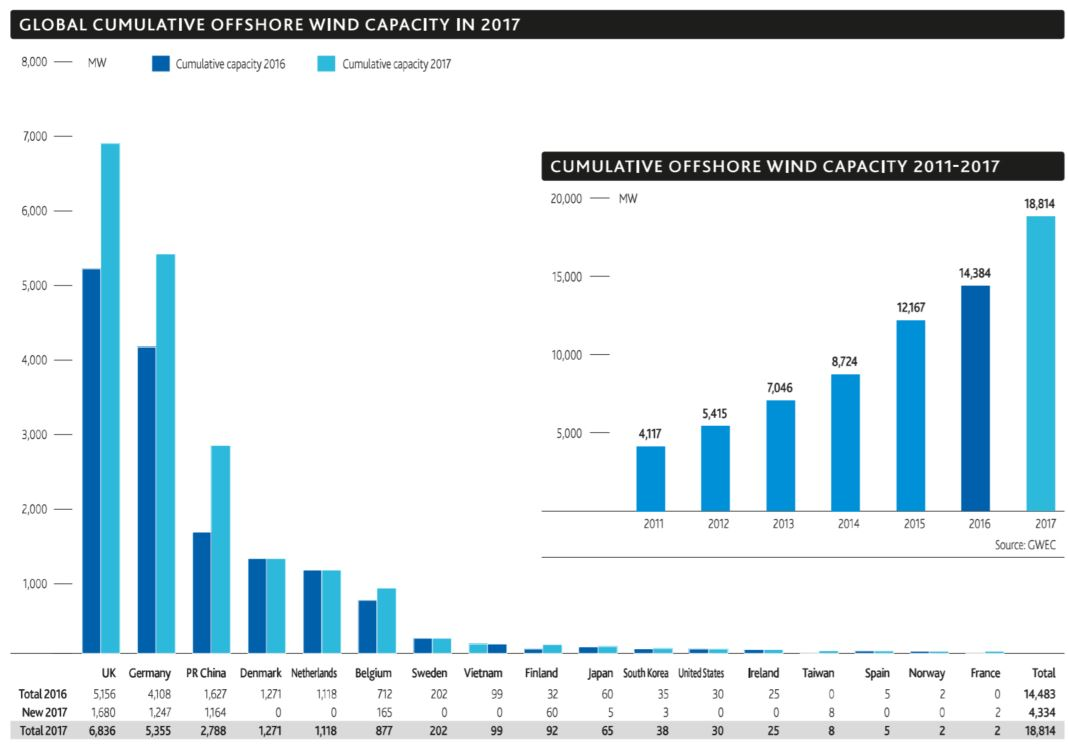
\includegraphics[scale=0.8]{figures/sit17}
\caption[$\; \:$Cumulative Offshore Wind Capacity in 2017]{Cumulative Offshore Wind Capacity in 2017 \cite{GWEC2018}}
 \label{fig:sit17}
\end{figure}

\noindent The majority of the offshore wind farms are located in Europe. Figure \ref{fig:world} shows the current market situation of offshore floating wind turbines. As can be seen, it is mainly Europe, USA, and China that are represented. 


\begin{figure}[H]
\centering
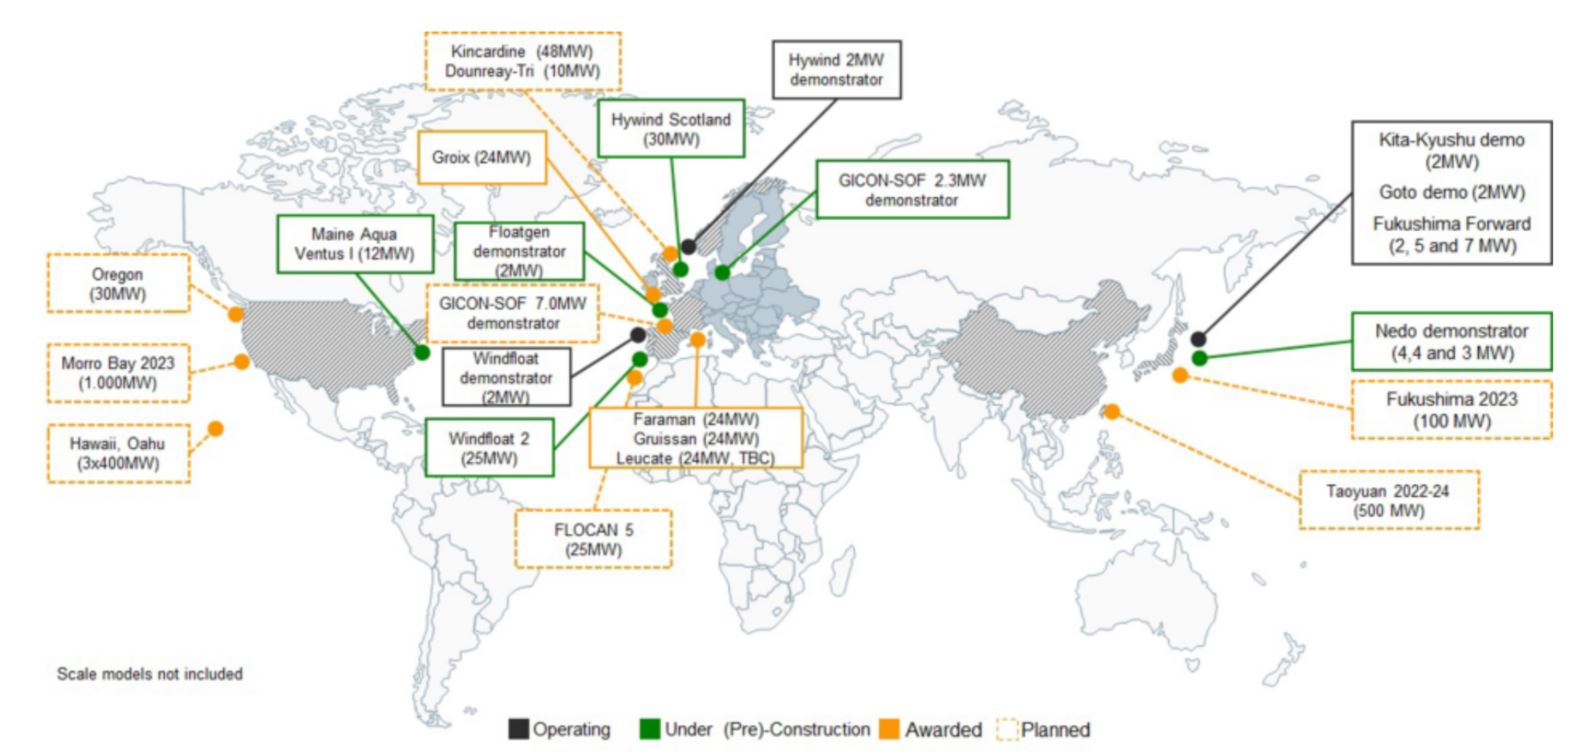
\includegraphics[scale=0.54]{figures/world}
\caption[$\; \:$Current market situation of offshore floating wind turbines]{Current market situation of offshore floating wind turbines \cite{Gao2018}}
 \label{fig:world}
\end{figure}

\noindent In the recent years, installations have moved further from shore, into deeper waters and with large farm configurations and larger turbines.  Longer blades will give advantages in terms of overall cost, but also challenges for installation, \cite{Gao2018}.  Figure \ref{fig:diameter} shows the development of power capacity for the last two centuries. The average size in 2017 was 5.9 MW. That is an increase of 23\% from 2016 according to \cite{we2018}.

\begin{figure}[H]
\centering
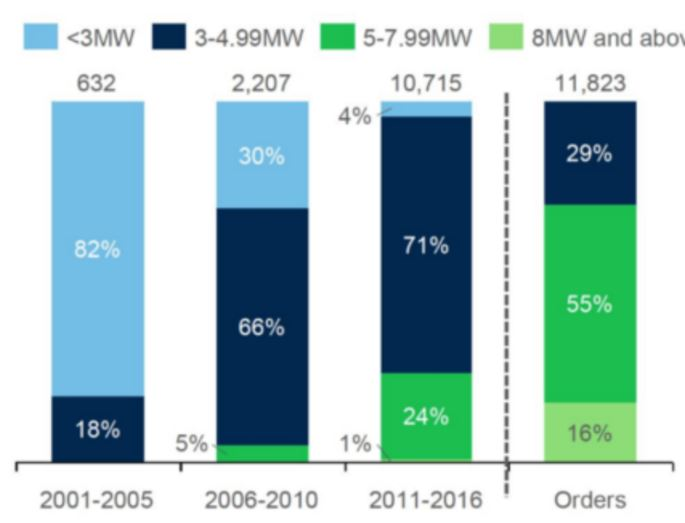
\includegraphics[scale=0.7]{figures/diameter}
\caption[$\; \:$Development of turbine size]{Development of turbine size. \cite{Deigen2018}}
 \label{fig:diameter}
\end{figure}

 \noindent In 2016, the first 8 MW turbine was installed in the Irish Sea in the UK. In Norway, Statoil made a step towards commercialization of floating wind farms by installing the first floating wind farm with 5 6MW spar wind turbines called Hywind, outside of Scotland. Hywind can be used at depths up to 800m, and enable offshore wind energy installations for areas that have been unavailable until now \cite{Equinor2018}. Short-term plans for the offshore wind industry include the installation of two small floating wind farms in the US as well as prototype testing for exiting prototypes in Norway, Portugal, and Japan, and planned prototype development in Japan, France, and Germany.  Two large wind farms are planned on the east coast of the US, one 120 MW farm outside of Maryland, and one 90 MW on the coast of New York. \cite{Gao2018}. \newline
 \newline
 \cite{Bailey2014} states that "Commercialization of floating wind farms is
anticipated between 2020 and 2025." In 2014 the European Union set a legally binding target that 27\% of the energy consumption are to come from renewable energy sources in 2030. \cite{EWEA2015}  presents three different scenarios on the development of offshore wind energy by 2030, and in the central scenario, it is suggested that 66 GW come from offshore wind. To achieve this goal, there needs to be an annual average increase of 15\%. \cite{Gao2018} states that this is probably possible as we have seen an increase of 25\%-30\% annually the recent years. US Department of Energy has a goal of 86 GW of energy provided from offshore wind by 2050. \cite{windus2016}. 
\subsection{Power Cables}
The trend over the years has been that offshore wind installations move further away from shore. This development can be seen in Figure \ref{fig:distshore}. 

\begin{figure}[H]
\centering
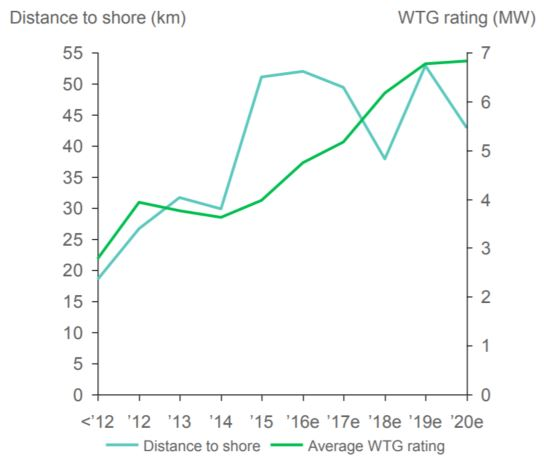
\includegraphics[scale=0.9]{figures/distshore}
\caption[$\; \:$Distance to shore ]{How distance to shore have increased in recent years \cite{Make2016}}
 \label{fig:distshore}
\end{figure}

\noindent \cite{srinil2016} states that traditionally, the w shape configuration has been used for inter-array cabling, and the lazy wave has been used for export cables, see Figure \ref{fig:cableconfig}. However, according to \cite{ds2010}, the lazy wave configuration is being considered for inter-array in newer projects such as the Statoil's Hywind project, and the Fukushima Floating Offshore Wind
Farm Demonstration Project, \cite{yagihashi2015dynamic}. Inter-array cables are usually three-core copper conductors, armoured with steel wires with insulation around the conductors. 33kV is usually the standard for offshore cables, however, 66kV are under development \cite{srinil2016}. 


\begin{figure}[H]
\subfloat[Traditional W-shape for inter array cable \label{fig:dc}]
  {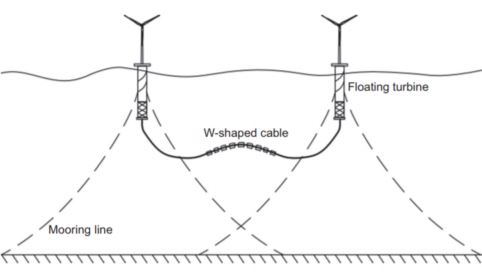
\includegraphics[width=.45\linewidth]{figures/wshape}}\hfill
\subfloat[Lazy wave shape, traditionally only used for export cables \label{fig:ac}]
  {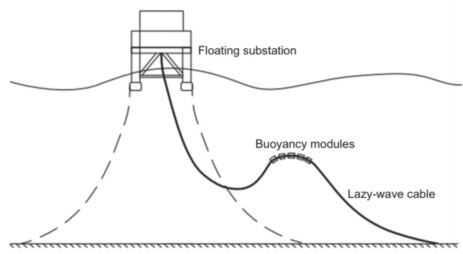
\includegraphics[width=.45\linewidth]{figures/lw}}\hfill
\caption[$\; \:$Cable configurations]{Different cable configurations, \cite{ds2010}}
\label{fig:cableconfig}
\end{figure}

\section{Objective}
\section{Contribution}


\section{Master Thesis Structure}

 % includes latex files from the same directory
\chapter{System Theory}
\label{chap:sysdes}
To understand the problem and the procedure to examine the fatigue of dynamic power cables in wind farms, a fundamental understanding of the system is required. This chapter covers theory for wind turbines in general and offshore wind turbines as well as subsea power cables. The chapter also includes historical background, some principal mathematical background, and other relevant theory. 
\section{Wind Turbines}
A wind turbine can convert kinetic energy into mechanical energy, and then to electric energy. This conversion is done by extracting the kinetic energy of an air stream by the use of a rotating, disk-shaped wind energy converter, \cite{Hau2013}.

\subsection{Historical Background of Wind Turbines}
According to \cite{Wagner2013}, man has utilized energy from the wind for thousands of years. In the earliest years, wind energy was mainly used as propulsion for sailing vessels. There are accounts of windmills in Persia as early as 914 AD, and in Europe from around 1200 BC. The first windmills were used for pumping of water and grinding of cereal. Between 1700-1800 there was a major spurge in windmill technology, and new designs with higher efficiency emerged. \cite{Lynn2011} states that before the industrial revolution, windmills were an important source of mechanical energy in Europe. Denmark, England, Germany, and the Netherlands were among the countries with the most development. Windmill technology experienced even more growth in the twentieth century, and in early 1900 multi-blade wind farms were developed in the US. At this time, the wind energy was used to convert kinetic energy into mechanical energy, \cite{Hau2013}. According to \cite{Lynn2011}, as the industrial revolution emerged, the advancement of windmills declined. Steam engines and combustion motors could provide power at any time, efficiently and independent of weather conditions. Electrical motors could be used to grind grains and pump water more effectively than ever. By the mid-1900s it was rare to see a traditional windmill still in service. \newline 
\newline
As electricity technology evolved, the notion of utilizing windmills to generate electrical power arose. One of the most remarkable people behind this approach was Charles Brush. As early as 1888 he developed "A multi-blade rotor 17 m in diameter, [...]a 12 kW dynamo charged a battery bank that fed various motors and hundreds of incandescent lights in his home over the next 15 years", \cite{Lynn2011}. This was the first \textit{wind turbine}. In the following years, there was enormous progress in the design and performance of wind turbines. \cite{Hau2013} describes the emergence of the modern wind turbine with the unit created by Ulrich Hütter. He published papers on the theory of wind energy in 1942 and is said to be one of the pioneers of modern wind energy technology. Hütter built wind turbines with fewer blades, that were profoundly aerodynamically refined, and designed for a greater rotation speed than was seen previously. According to \cite{Wagner2013}, this was particularly beneficial, as only a small generator was required to generate electricity. Figure \ref{fig:hutter} shows a windmill by Hütter, and as can be seen, it is quite similar to the windmills one usually encounters today. \newline
\newline

\begin{figure}[H]
\centering
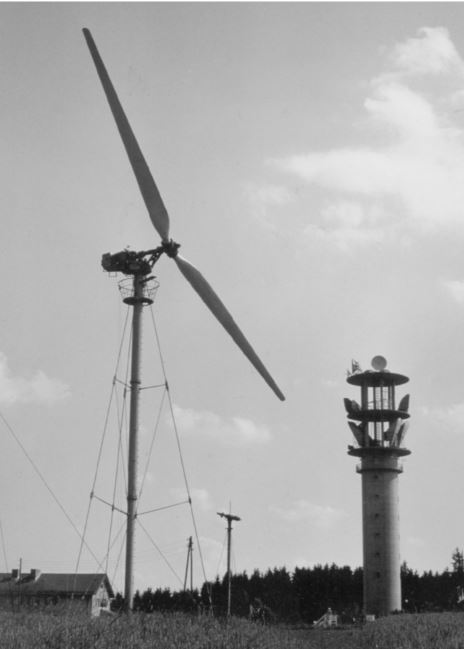
\includegraphics[scale=0.6]{figures/hutter}
\caption[$\; \:$Hûtter Wind Turbine Concept]{"Wind turbine by U. Hütter in Stötten in the Swabian Alb, Germany (rotor diameter 34 m, rated power 100 kW), 1958-1968" \cite{Hau2013} }
 \label{fig:hutter}
\end{figure}

\noindent \cite{Lynn2011} describes the 200kW wind turbine designed and built by the Dane Johannes Juul in 1957 as one of the most prominent concepts leading up to the modern wind turbine. It had stall control, and emergency aerodynamic tip breaks to avert damage in extreme weather. In 1975 it was refurbished by NASA to be used in their wind energy program. This turbine put Denmark on the map as one of the principal wind energy nations. 
\newline 
\newline
\noindent In spite of the dramatic increase in efficiency attained by the new technology, energy from wind turbines did not prove to be competitive compared to other sources of electricity in the 1960s to 1970s. It was not until the oil crisis in the seventies that several countries recognized that the world would eventually be dependent on other energy sources than fossil fuels sometime in the future, \cite{Wagner2013}.  President Jimmy Carter ensured the financing for several extensive wind projects, and by the early 1980s, the state of California had thousands of wind turbines with a combined power production of 1 GW. Nevertheless, this development stalled as President Reagan withdrew the financing of many projects, making Europe, and especially Denmark and Germany the leading nations in wind turbine technology. 
\cite{Lynn2011}

\subsection{Mathematical Background of Wind Turbines}
The concept of a wind turbine, independently of type, is to convert kinetic energy in the wind into mechanical energy, using a disk shape rotating wind energy converter. The mechanical energy is used to generate electrical energy.  According to \cite{Hau2013},  Albert Betz was the first to implement this principle to windmills, and developed theory where he applied elementary physics to wind converts. The theory contains simplifications such as assumed frictionless flow; however, it has demonstrated to be quite useful in the early stages of calculation for practical engineering. The following part of the section was originally developed by Albert Betz and later reproduced by \cite{Hau2013}.

\subsubsection{Basics of Albert Betz Momentum Theory:}
\noindent Kinetic energy:
\begin{equation}
    E=\frac{1}{2} m v^2 \qquad (Nm)
\end{equation}
 where for a wind converter, v is the velocity of an air flow of mass m. The volume flow, $\dot V$ is:
 
 \begin{equation}
    \dot V= v A \qquad (m^3/s)
\end{equation}
where A is the area. The mass flow $\dot m$ is expressed as:

 \begin{equation}
    \dot m = \rho_{air} v A \qquad (kg/s)
\end{equation}

\noindent where $\rho_{air}$ is the density of air. The amount of energy passing through the cross section per unit time:

 \begin{equation}
    P = \frac{1}{2}\rho_{air} v^3 A \qquad (W)
\end{equation}

\noindent  The kinetic energy in the airflow decreases with the extraction of mechanical energy. Reducing the velocity means widening the area of the cross-section. This is depicted in Figure \ref{fig:flow}. Here $V_1$ and  $A_1$ refers to the flow velocity and area before the extraction of energy, and $V_2$ and $A_2$ refers to the flow velocity and area after the extraction.

\begin{figure}[H]
\centering
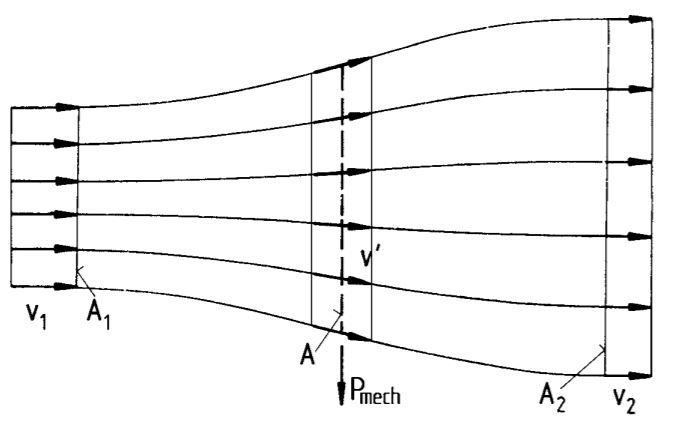
\includegraphics[scale=0.6]{figures/flow}
\caption[$\; \:$Changing flow conditions due to extracting of mechanical]{Changing flow conditions due to extracting of mechanical energy based on elementary momentum theory, \cite{Hau2013} }
 \label{fig:flow}
\end{figure}

\noindent The extraction of energy is due to the \textit{difference} in power before and after the extraction: 

\begin{equation}
    P = \frac{1}{2}\rho_{air} v^3_1 A_1 - \frac{1}{2}\rho_{air} v^3_2 A_2 =\frac{1}{2}\rho_{air}( v^3_1 A_1 - v^3_2 A_2) \qquad (W)
    \label{eq:air}
\end{equation}

\noindent From the Equation \ref{eq:air} it follows that the maximum energy extracted is obtained if $V_2=0$. Physically, however, this does not make sense as this implies that $V_1$ must become equal to zero, meaning no energy extraction at all. Through the conservation of momentum, Albert Betz developed a theory of the optimal relationship between the flow velocity before and after the extraction, $\frac{V_1}{V_2}$. $c_p$ is introduced to have a reference for the power output, where the power output, $P$  is compared the power of a free-flowing flow without extraction, $P_0$. 
  \begin{equation}
    C_P = \frac{P}{P_0}
\end{equation}

\noindent The following results were obtained: 

\begin{figure}[H]
\centering
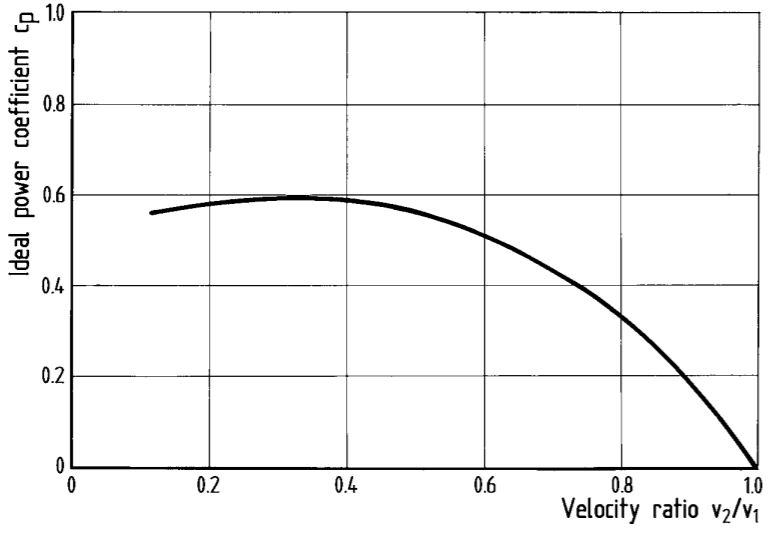
\includegraphics[scale=0.6]{figures/idealflow}
\caption[$\; \:$Power coefficient versus velocity ratio]{"Power coefficient versus velocity ratio" \cite{Hau2013} }
 \label{fig:idealflow}
\end{figure}

\noindent  From Figure \ref{fig:idealflow}, it is clear that the maximum power to be extracted is at $C_P$ close to 0.6, more precisely at 

 \begin{equation}
    C_P = \frac{16}{27} = 0.593
\end{equation}

\noindent This is frequently called the Betz factor and expresses the maximum theoretical efficiency. 

\subsubsection{Basics of Foil Theory}
One of the most fundamental components of the wind turbine are the blades. They are shaped as foils and are responsible for the transfer of the kinetic energy in the wind, to the mechanical energy of the rotor. \cite{MATHEW2012} states that in earlier days, the foils in wind turbines were adopted from airplane foils. Today,  there is a whole industry dedicated to the optimization and design of wind turbine foils. A basic illustration of the essential features of a standard airfoil is shown in Figure \ref{fig:foil}.  

\begin{figure}[H]
\centering
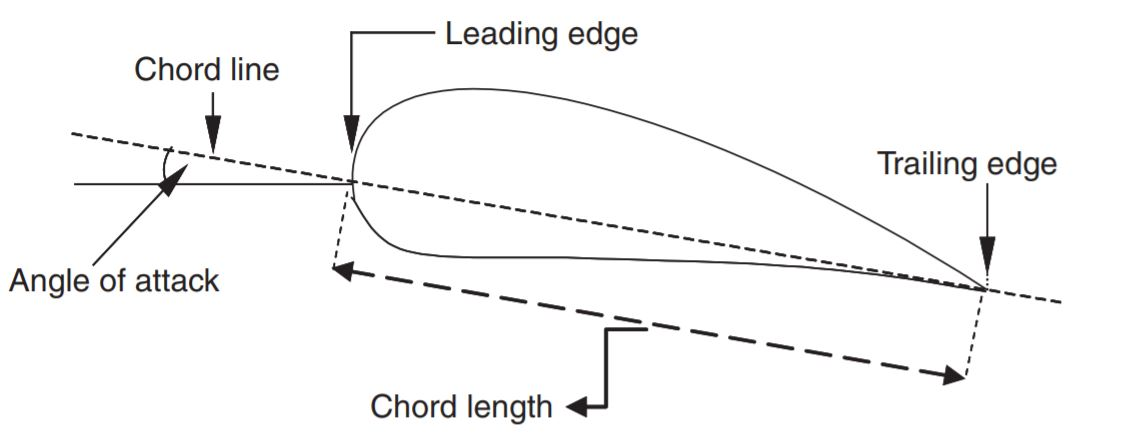
\includegraphics[scale=0.6]{figures/foil}
\caption[$\; \:$Basic features of a foil]{Basic features of a foil, \cite{MATHEW2012} }
 \label{fig:foil}
\end{figure}

\noindent If the foil is placed in a flow stream, the foil experiences a separation of streamlines above and below the foil. Due to the configuration of the foil shape, the streamlines above the foil have a longer way to travel than those below the foil. Because of this, the velocity of the flow on the upper side has to increase to meet the particles in the streamlines on the bottom of the foil at the trailing edge. According to Bernoulli's theorem, increased velocity has to be counterbalanced with a reduction in pressure. Decreased pressure creates a pressure difference between the upper and lower side of the foil resulting in a lift force directed upwards. At the same time, a drag force is also exerted on the foil. Their resultant is the net experienced force on the airfoil, as illustrated in Figure \ref{fig:liftdrag}, \cite{MATHEW2012}. 

\begin{figure}[H]
\centering
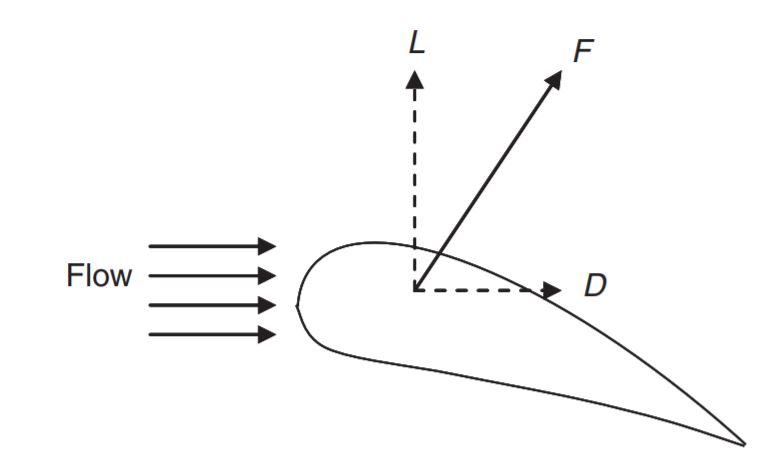
\includegraphics[scale=0.6]{figures/liftdrag}
\caption[$\; \:$Lift and drag on an airfoil]{Lift and drag on an airfoil \cite{MATHEW2012} }
 \label{fig:liftdrag}
\end{figure}

 \noindent The lift and drag can be expressed as:

 \begin{equation}
    L = C_L\frac{1}{2}\rho_{air} v^2 A \qquad (N)
\end{equation}

\begin{equation}
    D = C_D\frac{1}{2}\rho_{air} v^2 A \qquad (N)
\end{equation}
Where $C_L$ and $C_D$ are lift and drag coefficients respectively.\newline 
\newline

\noindent The angle of attack influences the lift and drag forces (see Figure \ref{fig:foil}). In terms of airfoils used in wind turbines, the drag force is just a parasite component following the lift force, so it is a goal to maximize lift and minimize the drag so that the ratio $\frac{C_L}{C_D}$ reaches its maximum. For a wind turbine, the rotation of the foils creates a tangential velocity. The velocity experienced by a point is the resultant of the velocity and the tangential velocity. The drag force is parallel with the resulting velocity, and the lift is always perpendicular to the drag. 

\section{Offshore Wind Turbines}
The following paragraph is taken from \cite{Kapsali2012}.\\\\ In later years, there has been a significant increase in wind power installations. Renewable energy is on high demand, and wind energy is considered a cost-effective way of providing it. As restrictions on wind installations increase in terms of noise and visibility, development is being withheld. This has made a new market emerge: Offshore Wind Energy. Offshore wind energy implies electrical energy generated by wind installation placed offshore.  There are several advantages of this: wind speeds tend to increase with distance from shore, giving offshore wind energy an even greater potential than on-land wind energy. Also, the noise and visibility of the wind turbines are no longer a problem as long as the installation is placed far enough from shore, and the environmental impact is minimal. However, there are several challenges as well. The wind industry is a relatively new industry, and the ocean conditions such as weather, waves, currents, corrosion, and more, pose several challenges and demands multidisciplinary cooperation for development of plausible designs. New approaches are needed in terms of turbine, structure, installation, and maintenance, and the cost of offshore wind energy is considered higher than on land. Offshore wind energy generally follows a simple rule: The further from shore an installation is placed, the greater energy potential in terms of wind speed, but this also implies deeper waters and increased development and operation costs. A lot of the experience gained from the oil and gas industry is valuable in the advancement of offshore wind energy. 

\subsection{ Historical Background for Offshore Wind Turbines}
\cite{NG2016} states that the first offshore wind farm was developed in Denmark in the 1990s. According to \cite{Lynn2011}, this wind farm consisted of 11 turbines providing 5 MW combined.  By using the already existing knowledge and technology both from the onshore windmill industry and the offshore oil and gas industry, offshore wind turbines have experienced rapid growth in the middle of the 2000s, with doubling of capacity every 2-4 years, \cite{NG2016}. Figure \ref{fig:development} shows the increase in offshore wind installations. \cite{Lynn2011} States that "It is reasonable that Europe will generate tens of gigawatts of offshore electricity by 2020".


\begin{figure}[H]
\centering
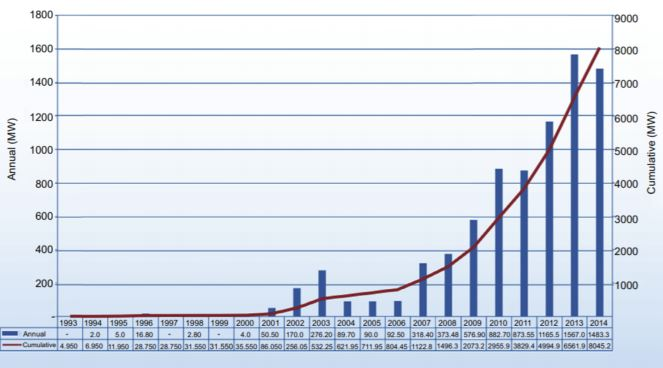
\includegraphics[scale=1.1]{figures/development}
\caption[$\; \:$Annual and cumulative offshore wind installations from 1993-2014]{Annual and cumulative offshore wind installations from 1993-2014 \cite{NG2016}}
 \label{fig:development}
\end{figure}


\subsection{Modifications for Offshore Wind Installations}
Offshore wind turbines are quite similar to onshore wind turbines, but with some modifications. Generally, offshore wind installations are larger to make use of the increased energy potential due to the high wind speeds. Concern for the public is also not a problem offshore, allowing larger installations that are more visible and noisier. Other alterations are necessary due to the harsh environment offshore. According to \cite{Kapsali2012}, this includes:
\begin{itemize}
    \item Strengthening of the tower to be able to handle the loads from the high wind speeds and wave loads form the ocean
    \item Corrosion systems to avoid corrosion from the salty water
    \item Warning lights and bright markers to avoid collision. 
\end{itemize}

\subsection{Offshore Support Structures}
Offshore wind turbines may be attached to the seabed or floating. According to \cite{IRENA2016}, the support structures that are attached to the seabed are restricted to water depths of 50m or less. As the offshore wind industry aims to move installations further offshore with increasing water depths, floating solutions are necessary. By introducing floating support structures, water depths constraints are eliminated (at least in terms of support structure). This opens new markets for countries with few shallow water areas suitable for offshore wind energy production. In most cases, moving further away from shore increases the wind speeds, and it also decreases the environmental impact on the surroundings. The main floating options are presented in Figure \ref{fig:supstruc}, are all familiar concepts from the oil and gas industry and have proven successful in demanding environments. 

\begin{figure}[H]
\centering
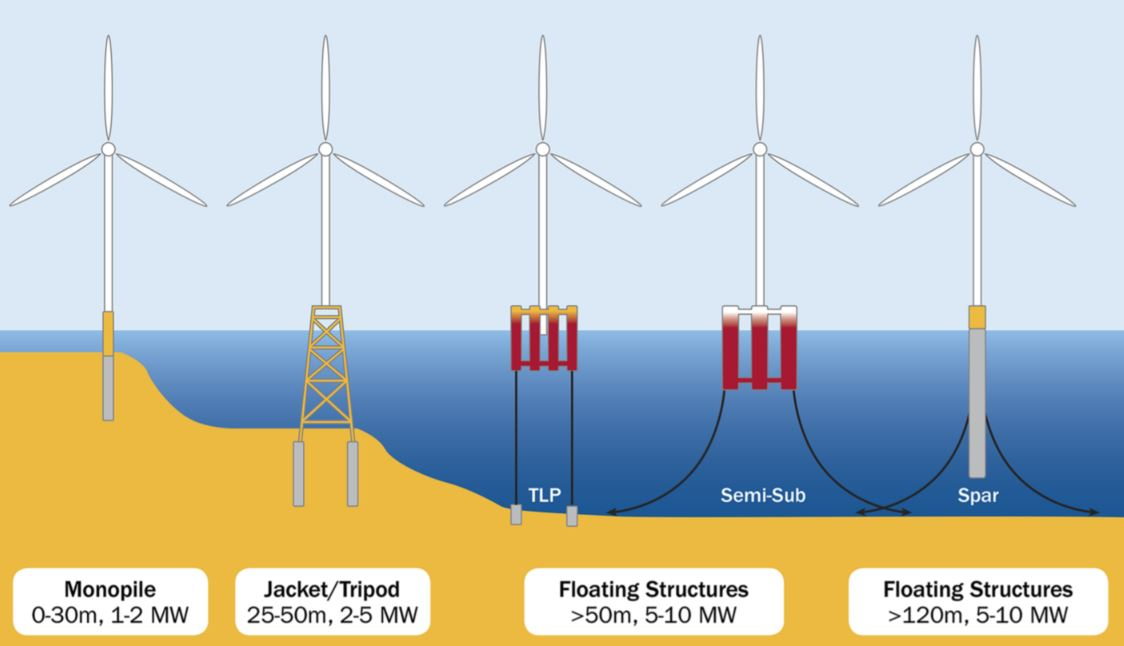
\includegraphics[scale=0.6]{figures/supstruc}
\caption[$\; \:$Different support structures]{Different support structures \cite{Bailey2014}}
 \label{fig:supstruc}
\end{figure}

\noindent There are several pros and cons to the different designs, taken from \cite{IRENA2016}: \newline
\newline
\textbf{Tension Leg Platform (TLP)}: Very buoyant structure connected to tensioned tendons secured to the seabed by piled or suction anchors.

\begin{varwidth}[t]{.5\textwidth}
Pros :
\begin{itemize}
\item Low mass
\item Lower critical wave induced motions
\item May be assembled onshore
\end{itemize}
\end{varwidth}% <---- Don't forget this %
\hspace{4em}% <---- Don't forget this %
\begin{varwidth}[t]{.5\textwidth}
Cons :
\begin{itemize}
\item Stability issues during installation and transportation
\item May need special purpose vessel for installation
\item Higher mooring cost
\item Some uncertainty around high frequency dynamic effects
\end{itemize}
\end{varwidth}
\newline
\newline

\noindent \textbf{Semi submersible}: Submerged pontoons. Kept in position by mooring lines

\begin{varwidth}[t]{.5\textwidth}
Pros :
\begin{itemize}
\item May be assembled onshore
\item Low drought, may be transported fully equipped using tugs.
\item Lower mooring costs 
\end{itemize}
\end{varwidth}% <---- Don't forget this %
\hspace{4em}% <---- Don't forget this %
\begin{varwidth}[t]{.5\textwidth}
Cons :
\begin{itemize}
\item Higher critical wave induced motions
\item Large structures, use more material
\item Complex fabrication
\item Higher mooring cost
\end{itemize}
\end{varwidth}
\newline 

\noindent \textbf{Spar Buoy}: A cylinder with high drought with ballast below the center of gravity. kept in position with mooring lines

\begin{varwidth}[t]{.5\textwidth}
Pros :
\begin{itemize}
\item Lower critical wave induced motions
\item Simple design.
\item Lower mooring costs 
\end{itemize}
\end{varwidth}% <---- Don't forget this %
\hspace{4em}% <---- Don't forget this %
\begin{varwidth}[t]{.5\textwidth}
Cons :
\begin{itemize}
\item Installation requires heavy lift vessel
\item Needs high water depths. 
\end{itemize}
\end{varwidth}


\section{Subsea Power Cables}
 The cabling system is a crucial component for the offshore wind energy installation. Electrical power cables are used in offshore wind technology to provide energy from the wind turbine to shore or the other way around. It can also be used to provide power to other installations at sea \cite{Nasution2013}.  \cite{srinil2016} describes that the cable industry has experienced a significant increase in the demand for subsea power cables. As technology pushes installations further from shore, and into deeper waters with tough conditions, technical advances are needed for the power cables as well. For safe and efficient transfer of electricity, cable designs must be optimized according to the location of the system, infrastructure, and technical properties. " [...]to significantly increase offshore wind capacity, the inter-array and export cabling systems have been identified by the offshore wind industry as one of the key areas where related cost savings should be considered."  \cite{srinil2016}. The design of offshore power cables has several technical and economic challenges, where the distance from shore is an important parameter. According to \cite{Lynn2011}, it is most economical to use 3-phase high-voltage AC transmission for distance up to 50 km.\newline
 \newline
 \cite{Thies2012} states that there is substantial experience with marine power cables due to the large oil and gas industry. However, there is little knowledge about the loading regimes for floating marine energy converters because the technology is still relatively new and is lacking experience. 
 \newline
 \newline
 There are several different cables in use to transport the generated electricity from the wind turbine to shore, or an offshore installation, illustrated in Figure \ref{fig:diffcable} This project focuses on the dynamic part of an inter-array cable between the floating structure and the seabed. 
 
 \begin{figure}[H]
\centering
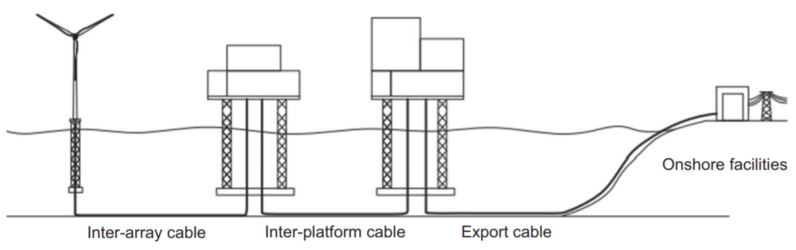
\includegraphics[scale=0.8]{figures/diffcable}
\caption[$\; \:$Different subsea power cable]{Different subsea power cables for different use. Adapted from   \cite{srinil2016} }
 \label{fig:diffcable}
\end{figure}

\noindent As can be seen in Figure \ref{fig:diffcable}, an inter-array cable link up several wind turbines to an offshore substation where the electricity is collected and transformed before it is sent to shore. \cite{srinil2016} describes that the inter-array cable is usually quite short, usually less than 1500m, depending on the size of the installation, and the spacing requirements between turbines. Inter-array cables are usually three-core copper conductors, armored with steel wires with insulation around the conductors. 33kV is usually the standard for offshore cables; however, 66kV is under development. \newline
\newline
  
  \subsection{Dynamic Power Cables}
According to \cite{Thies2012}, power cables can be used in static applications, where it is connected to a fixed structure, or dynamic application where it has to withstand significant cyclic loading. \cite{srinil2016} stats that "For offshore floating wind turbines, attention must be paid to the development, design, and optimization of a robust dynamic power cable." The combination of the different loads from waves, wind, currents, and more are complex and need to be assessed through a coupled model and experimental tests. \\\\
\subsection{General Design of Subsea Power Cable}
There are several different designs of subsea power cables. According to \cite{Beckman}, each cabling system is specially designed for its purpose, making repairs and maintenance challenging. \cite{Thies2012} describes some of the most common features for a standard subsea power cable presented in Figure \ref{fig:pcable}: 

\begin{enumerate}[label=\Alph*]
\item Conductor core: Carry the electrical current, and consists of wires made of copper or aluminum. 
\item Electrical insulation: Insulating the conductors. Possible materials are oil-impregnated paper, cross-linked polyethylene, or ethylene propylene rubber.
\item Sheath: Acts as a water barrier, and to protect the cable against fault currents. 
\item Armature: Metallic armature usually two layers of galvanized steel wires. Gives mechanical strength and protects against impact
\item Protective sheath: Outer layer of cable gives abrasion strength, and is made out of polypropylene
\end{enumerate}

\noindent Optical cables may be included in the cross section for some applications. Cables need to be optimized for their use, and standardized cables are rather rare. 


\begin{figure}[H]
\centering
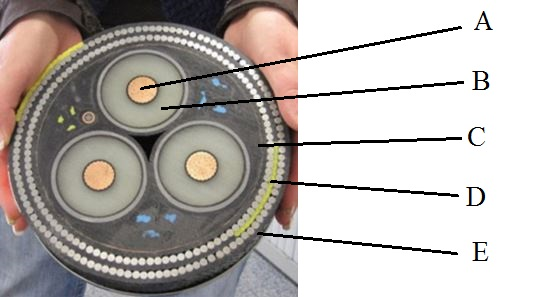
\includegraphics[scale=0.8]{figures/pcable}
\caption[$\; \:$Main components of a typical subsea power cable]{Main components of a typical subsea power cable. Adapted from  \cite{Boltinha2016} }
 \label{fig:pcable}
\end{figure}

\noindent As mentioned in section 1.3.2, the W-configuration is not the only configuration that has been used for inter-array cables in recent years, and other configurations are being explored. Figure \ref{fig:config} shows some of the most common riser configurations for floating offshore structures. 

\begin{figure}[H]
\centering
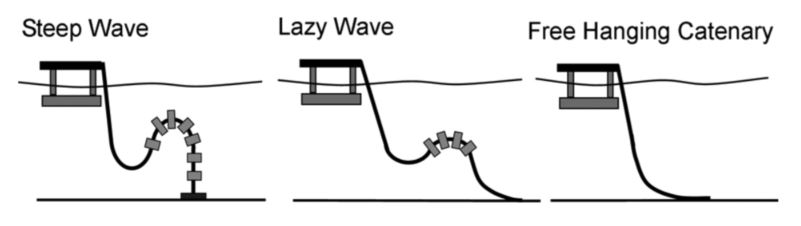
\includegraphics[scale=0.8]{figures/config}
\caption[$\; \:$Different configurations of flexible riser]{Different configurations of flexible riser \cite{Thies2012}}
 \label{fig:config}
\end{figure}

\noindent For the 1st and 2nd configuration in Figure \ref{fig:config}, buoyancy modules need to be designed to obtain the desired shape, according to \cite{srinil2016}. These are usually made of synthetic foam. They are positioned on the central part of the flexible riser/power cable and held in place with internal clamps. Using the steep wave or the lazy wave configuration usually minimizes the dynamic response of the cable,  decoupling the floating structure motion from the cable touch down point on the seabed. The configuration is highly dependent on the buoyancy elements, so these should not be changed over the lifetime of the flexible cable. Figure \ref{fig:bend} shows how buoyancy elements change the configuration of the flexible riser in terms of hang-off, arch bend, and touch down. "Depending on the hang-off angle, water depth, platform offset, footprint and soil stiffness, areas of local maximum static tensions typically occur at the hang-off point and
the two ends [...] of the distributed buoyancy portion[...]" \cite{srinil2016}. The local maximum bending moments happen where the largest curvature occurs.

\begin{figure}[H]
\centering
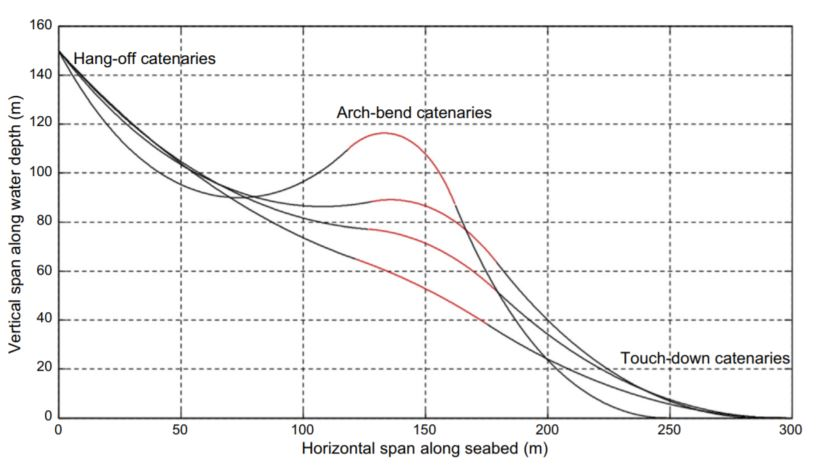
\includegraphics[scale=0.6]{figures/bend}
\caption[$\; \:$Effect of buoyancy distribution]{"Effect of buoyancy distribution (red line) change on the configuration of dynamic
cable" \cite{srinil2016}}
 \label{fig:bend}
\end{figure}
\subsection{Bend Stiffener}
The information in the following paragraph is taken from \cite{Worzyk}. \\\\
A dynamic power cable is susceptible to fatigue or over bend when there is an abrupt change in bending stiffness. This can be the case several places including at the cable hang off. An over-bend of the cable may lead to severe fatigue damage. To reduce the effect of changing bending stiffness, a bend stiffener may be incorporated in the cable structure. A bend stiffener is a conical structure attached around the cable at the cable hang off. Its conical shape makes the increase of bending stiffness more gradual, and each bend stiffener requires individual design. A poorly designed bend stiffener simply relocates the problem to the end of the bend stiffener.


\subsection{Copper Power Conductors}
  According to \cite{Worzyk}, the majority of subsea power cables include conductors made of copper. Copper is often superior to aluminum for subsea applications, as it allows for smaller cross-section, and thus requires less material for the steel armoring around it. There are several  types of conductors as can be seen in Figure \ref{fig:conductors}
  \begin{figure}[H]
\centering
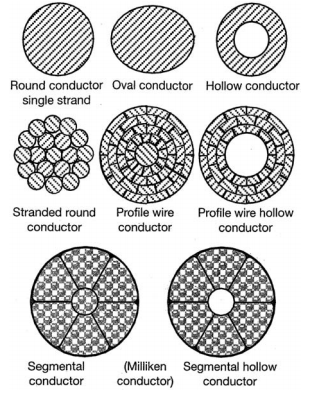
\includegraphics[scale=0.6]{figures/conductors}
\caption[$\; \:$Different types of conductors]{Different types of conductors, \cite{Worzyk} }
 \label{fig:conductors}
\end{figure}
 Stranded round cables are most prevalent for subsea application. \cite{Nasution2013} explains that the wires are arranged in layers, and the conductors may be of different sizes with a different number of layers. According to \cite{Worzyk} the wires are compressed in stranding machines in layers, or at the end of the stranding. The compression reduces the space between the circular wires, and a compressed copper cable may have a fill factor up to 0.92. 
  \\\\
 \cite{Nasution2013} elaborates: The helical nature of the wires in each layer leads to different contact between the wires. Contact between wires of the same layer is called inline contact, while contact between wires of different layers is called trellis contact. The inline and trellis contact between the wires can be seen in Figure \ref{fig:cross}, where the red arrows indicate inline contact, and the black arrows indicate trellis contact. 
  \begin{figure}[H]
\centering
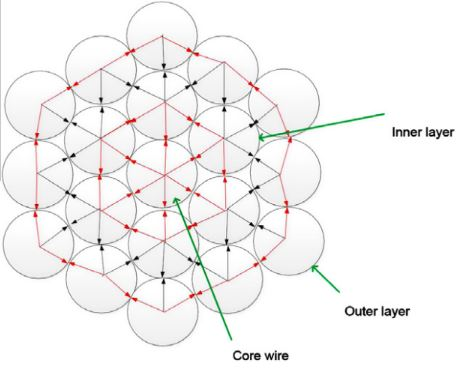
\includegraphics[scale=0.9]{figures/cross}
\caption[$\; \:$Inline and trellis contact between wires]{Inline and trellis contact between wires \cite{Nasution2013} }
 \label{fig:cross}
\end{figure}

\noindent The loads on the cables are transferred to the individual wires in the copper conductor. The dynamic and mean tension, are transferred as tension and shear force, and the dynamic bending moment gives local bending and axial friction forces. This can be seen in Figure \ref{fig:cable}, where:
\begin{itemize}
    \item $\overline T$ is the mean tension
    \item $\Delta T$ is the dynamic tension
    \item $\overline M_T$ is the mean bending moment
    \item $\Delta M_T$ is the dynamic bending moment
    \item $\Delta \beta$ is the dynamic curvature
    \item $\overline F_X$ is the mean axial force
    \item $\Delta F_X$ is the dynamic axial force
    \item $\overline T$ is the mean tension
    \item $\Delta M_X$ is the dynamic torque moment about helix tangential x-direction
    \item $\Delta M_y$ is the dynamic bending moment about helix bi-normal y-direction
    \item $\Delta M_z$ is the dynamic bending moment about surface normal z-direction
\end{itemize}


\begin{figure}[H]
\centering
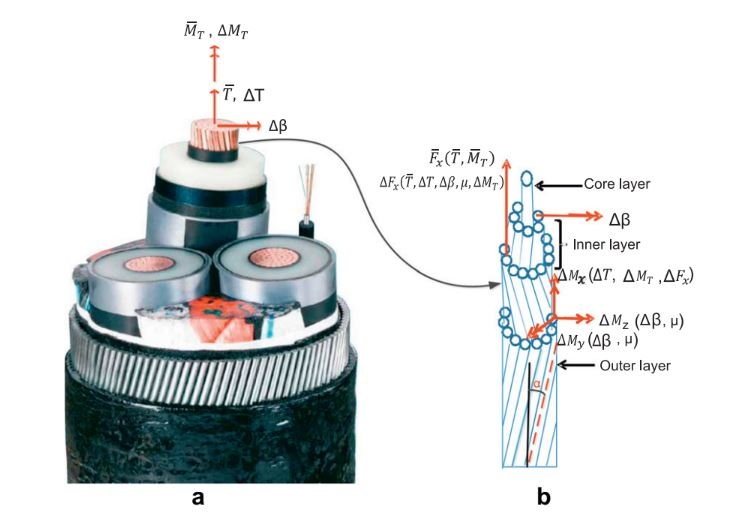
\includegraphics[scale=0.8]{figures/cable}
\caption[$\; \:$Forces on cable]{Forces on cable  \cite{Nasution2013} }
 \label{fig:cable}
\end{figure}

\subsection{Alternating current (AC) Voltage}
Electrical power can be supplied either by direct current, (DC) or alternating current, (AC). DC only flows in one direction, while for AC, the direction of the current changes direction several times over a time unit as a sine function, \cite{Dale2000}. Figure \ref{fig:acdc} compares the waveform for DC current and AC current.


\begin{figure}[H]
\subfloat[Waveform for DC voltage \label{fig:dc}]
  {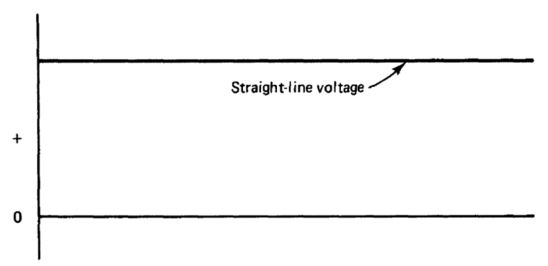
\includegraphics[width=.45\linewidth]{figures/dc}}\hfill
\subfloat[Waveform for AC voltage \label{fig:ac}]
  {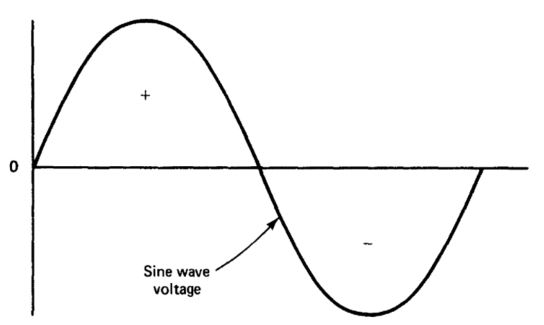
\includegraphics[width=.45\linewidth]{figures/ac}}\hfill
\caption[$\; \:$Comparison of DC voltage and AC voltage]{Comparison of DC voltage and AC voltage, \cite{Dale2000}}
\label{fig:acdc}
\end{figure}

\noindent A three-phase system is made up of three coils rotating in a magnetic field with a phase difference of 120$^{\circ}$, \cite{Dale2000}. The three-phase system and its alternating voltage can be seen in Figure \ref{fig:volt}. According to \cite{Beckman}, an AC cable requires one conductor for each phase. The three conductors may be placed in the same cable or within three individual cables. AC demands a thicker cable cross-section than DC, but smaller transformers.

\begin{figure}[H]
\subfloat[Single phase AC voltage \label{fig:single}]
  {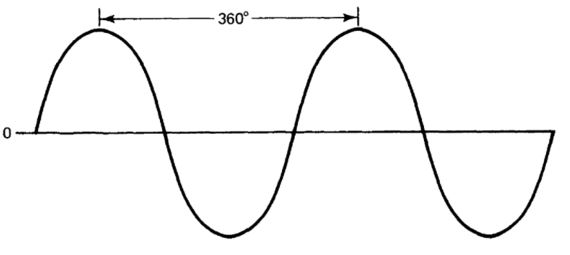
\includegraphics[width=.45\linewidth]{figures/single}}\hfill
\subfloat[Three phase Ac voltage \label{fig:3phase.JPG}]
  {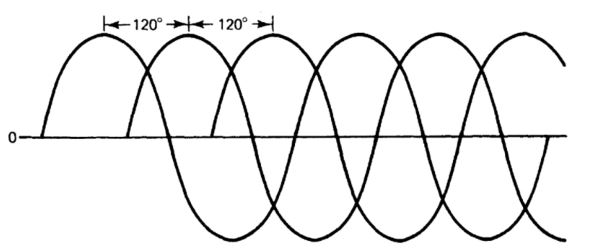
\includegraphics[width=.45\linewidth]{figures/3phase}}\hfill
\caption[$\; \:$Comparison of single phase and three phase AC voltage]{Comparison of single phase and three phase AC voltage, \cite{Dale2000}}
\label{fig:volt}
\end{figure}

\noindent There are several advantages with three-phase AC systems over 1 phase AC systems in terms of price, material use, robustness,"[...] and accounts for the vast majority of the world's industrial machines", \cite{1995Tac}.
 


 % could be called Methodology or methods or any filename  % could be results% could be results
\chapter{Fatigue due to Environmental Loads}
\label{chap:fatigue}
In the case of a floating wind turbine, environmental loads that will work on the model includes waves, wind, current and more. In this project/master thesis the focus will be on wave loads. Due to the cyclic nature of waves, failure of a dynamic power cable applied in offshore wind farms can be caused by either overloading or fatigue. In this master/project thesis the focus will be on failure due to fatigue. This section will attempt to explain the basic principles on how waves can give fatigue damage for a dynamic power cable attached to a floating wind turbine, as can be seen in the simple flowchart in Figure \ref{fig:flowchart}. 

\begin{figure}[h!]
\centering
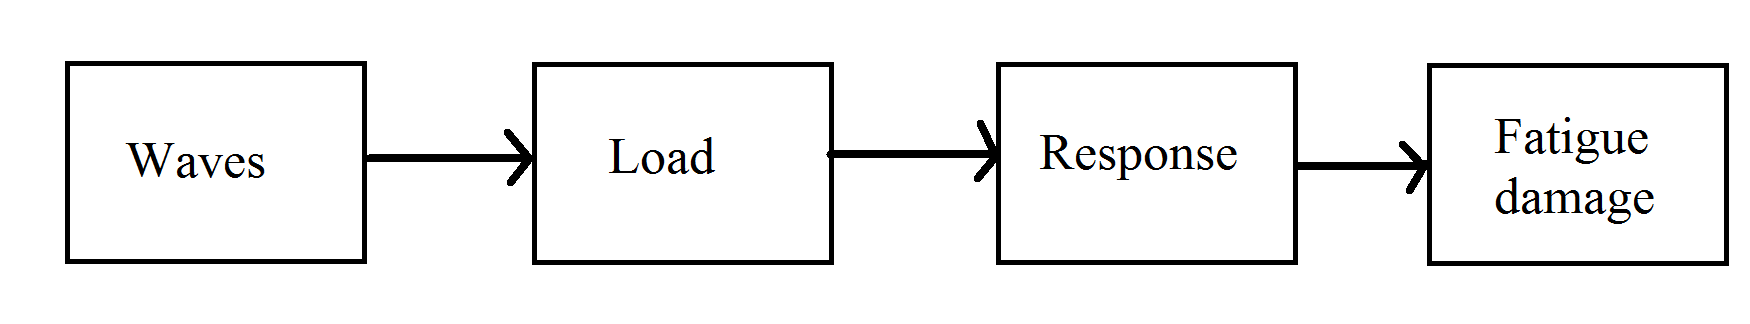
\includegraphics[scale=0.4]{figures/box}
\caption[$\; \:$Flowchart]{Flowchart for how waves can give fatigue damage in floating structure}
 \label{fig:flowchart}
\end{figure}

\section{Statistical Description of Waves} 
 The theory in this section is taken from \cite{Faltinsen1990}. For linear theory, the results from irregular waves can be obtained by adding together results from regular waves. For long-crested irregular sea, the wave elevation can be described as:
\begin{equation}
    \zeta = \sum_{j-1}^N A_j \sin(\omega_jt-k_jx+\epsilon_j)
    \label{eq:elevation}
\end{equation}
Where $\omega$ is the circular frequency, $t$ is time, $k$ is the wave number, $\epsilon$ is phase and $A$ is the the amplitude that can also be expressed in terms of the wave spectrum:
\begin{equation}
    \frac{1}{2}A_j=S(\omega_j) \Delta \omega
\end{equation}
Where $\Delta \omega$ is the difference between successive frequencies. The wave elevation is Gaussian distributed with mean at zero and $\sigma^2= \int_0 ^ \infty S(\omega) d\omega $. The wave spectrum assumes that the sea can be described as a stationary random process, meaning that it is a short-time description of the sea state. The sea state is defined by the significant wave height, Hs and the peak period, Tp. Hs is the mean height of the $\frac{1}{3}$ highest waves in the sea state, and Tp is the peak frequency of the wave spectrum. There exist several different spectrums but according to \cite{Lifes50+D1.1}: the JONSWAP (Joint North Sea Wave Project) is suitable for "wind seas", and thus this is what will be used in this case. The JONSWAP spectrum can be described as:
\begin{equation}
    S(\omega)=155 \frac{H_s^2}{T_1^4 \omega ^5} \exp{(\frac{-994}{T_1^4 \omega ^4})} 3.3^Y
\end{equation}
Where
\begin{equation}
    Y= \exp \left(-\left( \frac{0.191 \omega T_1 -1}{2^\frac{1}{2} \sigma} \right)^2\right)
\end{equation}

\begin{figure}[H]
\subfloat[General Wave Spectrum \label{fig:lm_total}]
  {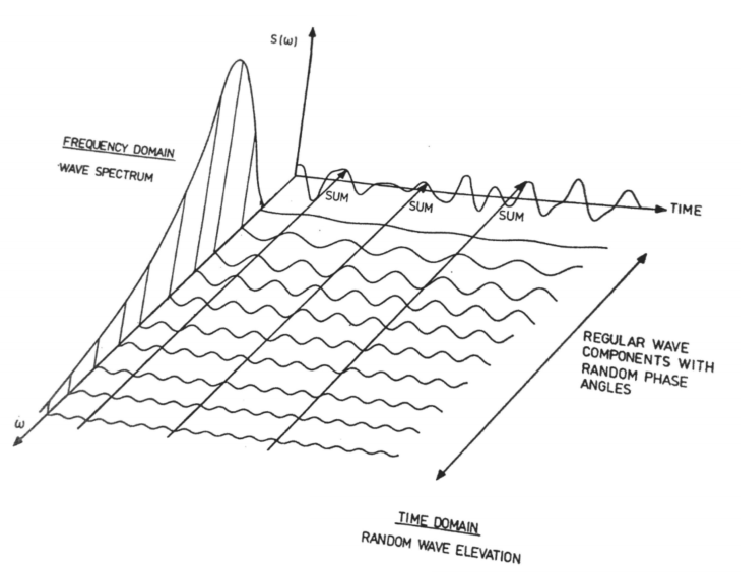
\includegraphics[width=.45\linewidth]{figures/spectrum}}\hfill
\subfloat[JONSWAP Wave Spectrum \label{fig:lm_cross}]
  {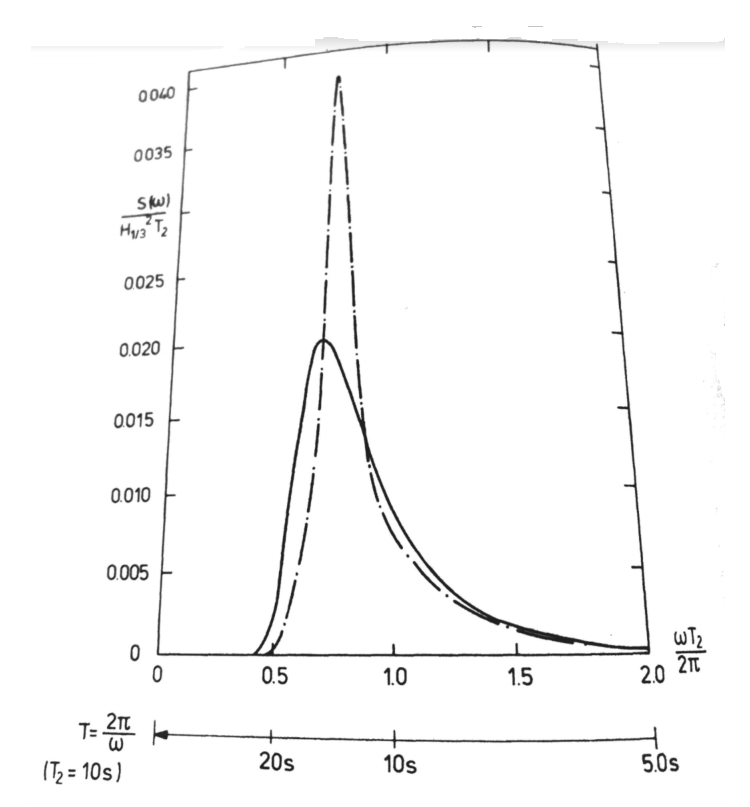
\includegraphics[width=.35\linewidth]{figures/JONSWAP}}\hfill
\caption[$\; \:$General wave spectrum and JONSWAP Spectrum]{General wave spectrum and JONSWAP Spectrum \cite{Faltinsen1990}}
\label{fig:spectrum}
\end{figure}

\noindent The long-term sea state is often described in a scatter diagram featuring the number of occurrences for different Hs and the Tp.  \newline
\newline\newline

\section{Load from Waves}
The loads from the waves acting on the floating wind turbine can be calculated using Morison's Equation. The general Morison's Equation expresses the horizontal force dF on a strip of the length dz of a fixed vertical cylinder and is formulated in \cite{BP2007} as:
\begin{equation}
    dF=\rho \frac{\pi D^2}{4} C_M a_x dz +\frac{1}{2} \rho C_D Du |u|dz
    \label{eq:morison}
\end{equation}
\noindent Where $\rho$ is the density of the water, D is the diameter of the pipe, $C_M$ is the mass coefficient, $a_x$ is the horizontal particle acceleration, is the acceleration in x direction, $C_D$ is the drag coefficient and u is the horizontal particle velocity. \newline
\newline
\newline
In the case of a moving cylinder, the Morison's Equation can be modified according to \cite{Faltinsen1990} as follows:
\begin{equation}
    dF=\frac{1}{2}\rho C_D D dz(u-\dot{\eta_1}) |u-\dot \eta_1| +  \rho C_M \frac{\pi D^2}{4} dz a_1 -\rho (C_M-1) \frac{\pi D^2}{4} dz \ddot{\eta_1}
    \label{eq:movemorison}
\end{equation}
Where $u$ and $a_1$ depend on position and dot represents time derivative.
\section{Response}
\cite{Langen1999} explains that an arbitrary loading can be written as a sum of harmonic components, and these can be Fourier-Transformed so that the contribution from each of the components will be a function of $\omega$. The response can also be transformed into the frequency domain, and this will give a direct measure of how the structure responds to different load frequencies. "Solution in the frequency domain is particularity suited for analysis of the response to stochastic loads [...]" \cite{Langen1999}. 
 
\begin{figure}[H]
\subfloat[Transformed excitation\label{fig:transex}]
  {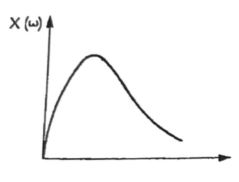
\includegraphics[width=.3\linewidth]{figures/transex}}\hfill
\subfloat[Transfer function \label{fig:cavS2500}]
  {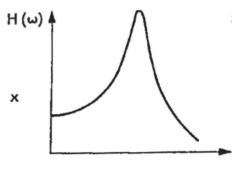
\includegraphics[width=.3\linewidth]{figures/transex2}}\hfill
  \subfloat[Transformed response \label{fig:cavS5000}]
  {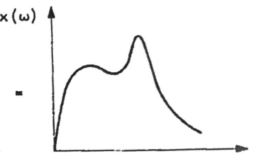
\includegraphics[width=.3\linewidth]{figures/transex3}}\hfill
\caption[$\; \:$Solution in the frequency domain]{Solution in the frequency domain, \cite{Langen1999}}
\label{fig:transex}
\end{figure}

\noindent Motion transfer functions give an efficient description of the motion characteristics of a floating vessel. They are calculated for all 6 degrees of freedom on a specified point on the vessel from either potential theory or experimental tests. \cite{sintef2017}. Due to linearity, the response can be analyzed for each wave component in equation \ref{eq:elevation} separately, \cite{Faltinsen1990}. Recalling equation \ref{eq:elevation}, for wave elevation, the steady state response can be written as:

\begin{equation}
    A_j |H(\omega)|\sin(\omega_jt-\delta_j(\omega)+\epsilon_j)
\end{equation}
Where $|H(\omega)|$ is called the transfer function. For irregular sea, the response can be linearly superposed for all the different wave components:
\begin{equation}
    \sum_{j=1}^N  A_j |H(\omega)|\sin(\omega_jt-\delta_j(\omega)+\epsilon_j)
\end{equation}
 $|H(\omega)|$ and $\delta(\omega_j)$ are functions of frequency, $\omega$.\newline 
 \newline


\noindent In this project/master thesis the results from the global analysis will be expressed as time series, in the time domain, and Fourier transformations are necessary to convert the response from the frequency domain to the time domain. \newline
\newline 
\noindent For the global model in SIMA RIFLEX, the transfer functions of OO-Star have been provided by Dr. Techn. Olav Olsen, to simulate the motions of the vessel when subjected to waves. As the transfer functions are regarded as confidential they cannot be reproduced in this project thesis report.   

\section{Fatigue}
Fatigue is damage due to cyclic loading over time where the stress is usually lower than the yield stress for a given material. In this section, some basic concepts related to fatigue will be presented, as well as some methods that are to be used in this master thesis. The following is taken from the compendium by \cite{fatigue2016}. \newline
\newline
\subsection{Basic Concepts}
In Figure \ref{fig:fatigue} some basic concepts are defined. 

\begin{figure}[h!]
\centering
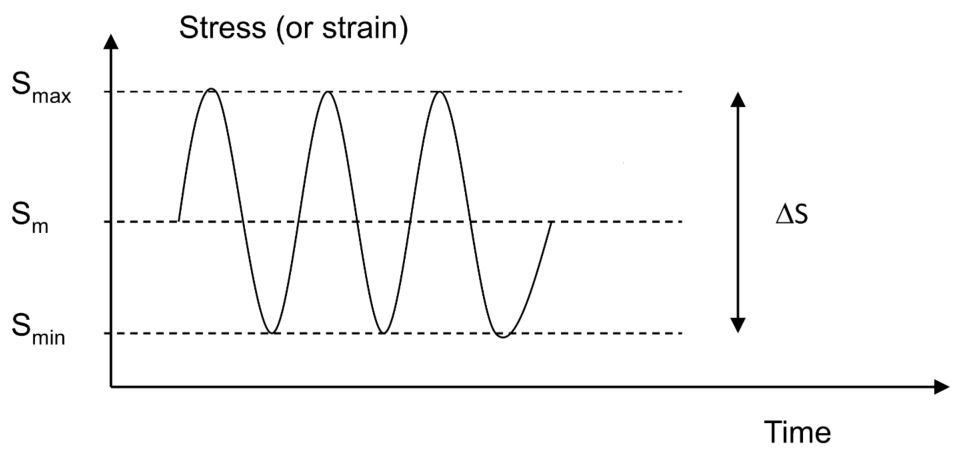
\includegraphics[scale=0.6]{figures/cycle}
\caption[$\; \:$Example of fatigue load history]{Example of fatigue load history  \cite{fatigue2016} }
 \label{fig:fatigue}
\end{figure}

From this Figure, it can be seen that:
\begin{itemize}
    \item $S_{max}$ -  Max stress/strain in a cycle
    \item $S_{min}$ -  Min stress/strain in a cycle
    \item $S_{m}$ - Mean stress/strain in a cycle
\end{itemize}

From this it follows that the stress range, $\Delta S$ is:

\begin{equation}
    \Delta S =S_{max} - S_{min}
\end{equation}

\noindent And the stress ratio, R is:
\begin{equation}
    R=\frac{S_{min}}{S_{max}}
\end{equation}
Fatigue data can be plotted in an SN diagram where stress or strain range is plotted against the number of cycles until failure, as can be seen in Figure \ref{fig:sn}. For most applications, fatigue life spans over a high number of cycles, so the SN plot is presented as a log-log-diagram. It is common to differentiate between high cycle fatigue and low cycle fatigue, where high cycle fatigue has a fatigue life at more than $10^5$ cycles, and the stress is elastic. High cycle fatigue tends to follow a log-linear relationship called the SN curve:
\begin{equation}
    N(\Delta s)^m = \text{c}
\end{equation}
\label{eq:sn}
Where N is the number of cycles before failure, $\Delta S$ is the stress range, m is an exponent and c is a constant.\newline
\newline
For the low cycle fatigue, the material will experience plastic deformation. For marine structure applications, the stress is usually in the high cycle fatigue range. If the stress range is sufficiently low, fatigue life can approach "infinite". This is called the fatigue limit and only applies in non-corrosive environments. 

\begin{figure}[h!]
\centering
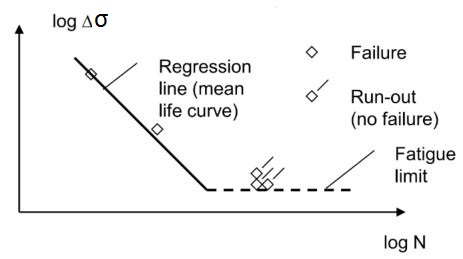
\includegraphics[scale=1]{figures/sn}
\caption[$\; \:$Example of SN curve]{Example of SN curve  \cite{fatigue2016} }
 \label{fig:sn}
\end{figure}

 \noindent The damage done by one cycle is usually close to insignificant, and undetectable by instruments. Failure due to fatigue is a result of the cumulative damage done by the cyclic loading. For marine structures, load from waves, current, motions, and vortex-induced vibrations may cause severe damage. Fatigue damage can be divided into three stages:
 \begin{itemize}
     \item Crack initiation, $N_i$
     \item Crack growth, $N_g$
     \item Failure
 \end{itemize}
 This means that the fatigue life can be calculated as:
 \begin{equation}
     N=N_i+N_g
 \end{equation}
 
\subsection{Irregular Loading}
For marine structures, it is common that the loading is irregularly cyclic, see Figure \ref{fig:irr}, where the amplitude and frequency vary over time. The lifespan for a typical specimen in the offshore industry is 20 years with an average frequency at 16 1/s. To make design process manageable, this has to be reduced to a more practical format.  

\begin{figure}[H]
\centering
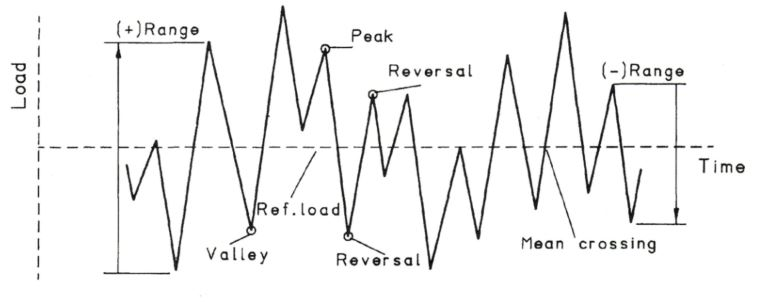
\includegraphics[scale=0.8]{figures/irr}
\caption[$\; \:$Example of irregular loading]{Example of irregular loading  \cite{fatigue2016} }
 \label{fig:irr}
\end{figure}

In Figure \ref{fig:irr}, a few concepts of irregular loading are defined:
\begin{itemize}
\item Reversal - Where the first derivative changes sign
    \item Peak - Where the first derivative changes from positive to negative sign
    \item Valley - Where the first derivative changes from negative to positive sign
    \item Range - Difference between a peak and a valley
    \item Mean crossing - number of time the load-time history crosses the mean load level (normally only crossings with positive first derivative is counted
    \item Bandwidth - Ratio of mean crossings with positive slope to the number of peaks or valleys. 
\end{itemize}
 
\subsubsection{Rain flow counting}
\label{sec:rainflow}
There are several ways of counting cycles, and rain flow counting is one of them. The name of this method stems from the thought of rain falling on the roof of a pagoda (Chinese architecture). In this procedure, the reversals are counted in accordance with the stress-strain response. This can be seen in Figure \ref{fig:count}, where the cycle from 2-3-2' does not affect the rest of the stress-strain cycle. Each time a loop is completed, a cycle count is made. This means that the counting of the cycles are reflecting the way the material is responding. The fatigue damage caused by a closed loop in the irregular amplitude loading is, according to this counting method, the same as one cycle in a constant amplitude test. Half cycles cannot be paired up with other half cycles, so the damage they do on the structure is not counted in this method, but in a realistic case, there will be few half cycles. Due to its versatility, the rain flow method is considered a superior method to the other counting methods. 

\begin{figure}[H]
\centering
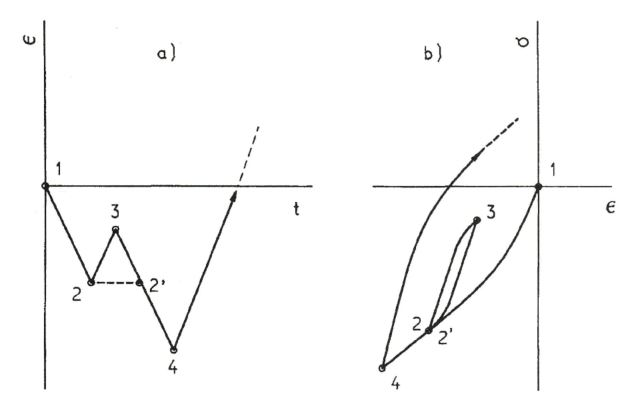
\includegraphics[scale=0.6]{figures/count}
\caption[$\; \:$Cyclic load and stress-strain response]{(a)Cyclic load (b) Stress-strain response.   \cite{fatigue2016} }
 \label{fig:count}
\end{figure}

\noindent Figure \ref{fig:pagoda} shows the rain flow counting method method:\newline 
\newline
Begin at the first valley. If the next valley is deeper or equal to the first one, the rain flow stops here and a cycle is counted, (see point 5 in the Figure). If the valley is not deeper than the first one, the flow proceeds to the next valley, (see point 3 in the Figure). The rain-flow is also considered to stop if it meets another flow from above, (see point 2' in the Figure) When one rain flow has stopped, proceed to the next valley and repeat the procedure. When this has been done to all the valleys, do the same for all the peaks. The results from the rain flow counting can be gathered in a histogram that easily will show the number of cycles for different levels. 

\begin{figure}[H]
\centering
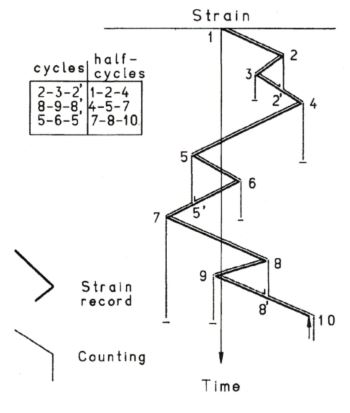
\includegraphics[scale=0.9]{figures/pagoda}
\caption[$\; \:$Rain flow counting]{Rain flow counting with illustrating the Chinese pagoda origin.    \cite{fatigue2016} }
 \label{fig:pagoda}
\end{figure}

\subsection{Cumulative Damage}
Several methods can be used to calculate the cumulative damage due to irregular amplitude cyclic loading. Miner-Palmgren approach has proven to be as good as other methods and is extremely simple. The Miner-Palmgren theory assumes that the damage is constant during a given stress range. The Miner-Palmgren expression:
\begin{equation}
    D=\sum_i \frac{n_i}{N} 
    \label{eq:MP}
\end{equation}
Where $n_i$ is the number of cycles with a certain stress range experienced by the structure and N is the fatigue life of at that stress range.\newline
\newline
The specimen will fail due to fatigue if D exceeds 1.

\subsection{Fatigue of Dynamic Power Cables}
\noindent According to \cite{Nasution2013}, when the cable is in operation, it will experience loads from gravity, the motions of the floating vessel, and from the sea. The cable will experience a mean global tension and torque due to the gravity. Surge and heave motion will induce dynamic tensile and torque, while pitch and roll motion will give a dynamic curvature of the cable. This can be seen in Figure \ref{fig:float}. 

\begin{figure}[H]
\centering
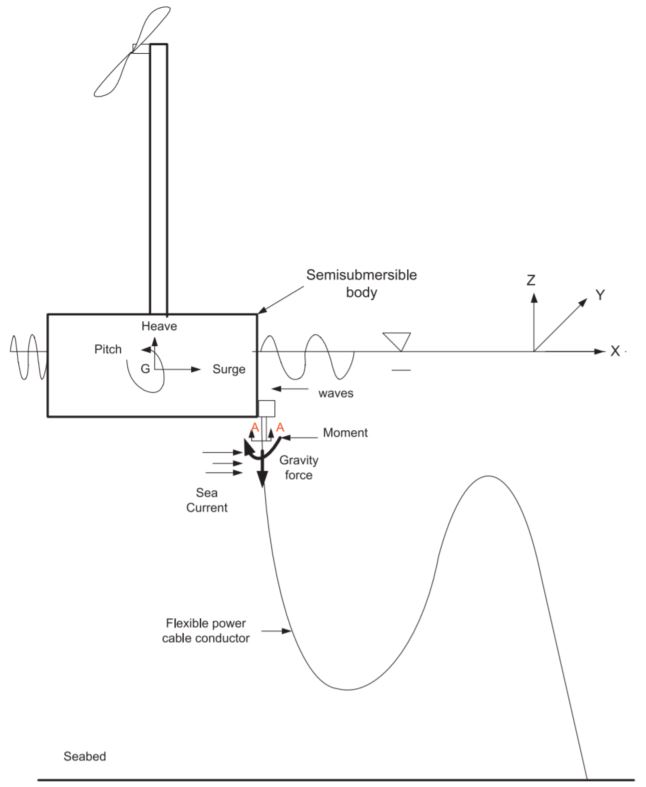
\includegraphics[scale=0.7]{figures/float}
\caption[$\; \:$Dynamic flexible power cable attached to semi-submersible wind turbine]{Dynamic flexible power cable attached to semi-submersible wind turbine \cite{Nasution2013}}
 \label{fig:float}
\end{figure}
\noindent \cite{YangShun-Han2017} states that fatigue life is an important parameter in determining service life for a subsea a power cable. \cite{Thies2012} says that power cables can be used in static applications, where it is connected to a fixed structure, or dynamic application where they have to withstand significant cyclic loading. Due to this, dynamic power cables are subjected to fatigue failure.
There are mainly three reasons for mechanical failure in marine power cables applied to marine energy applications, taken from \cite{Thies2012} :

\begin{itemize}
    \item Maximum axial tension
    \item Over bending
    \item Fatigue under extreme cyclic loads
\end{itemize}

\noindent According to \cite{Karlsen2010}, the individual wires and the intersection between them is what determines the fatigue properties of a copper conductor. R-ratio of loading and wire interaction have been recognized as important factors to fatigue life in copper conductors, and fretting fatigue (fatigue due to oscillating load on a junction between two components \cite{Hills1994}) is identified as one of the dominating mechanisms in a multi-layer stranded steel wire. Friction force increases with increasing lay angle and friction coefficient for the material. The copper conductors do not only have contact between conductor surfaces, but also with the protecting sheath around the conductors, giving a complex friction situation. 

\subsubsection{Fatigue of Copper Conductors}
According to a study done by \cite{Nasution2013}, when testing individual wires as well as a full cross-section of a three-phase 95mm$^2$, all failures occurred in the inner layer for the cross-section bent over a bell mouth. In addition, individual wires from the outer layer of the cross section were tested in controlled tension-tension loading. Here, all initiation of crack growth happened within or at the edge of the trellis contact area, that has been deformed due to the compacting process of the cable. The study concludes with that the difference in fatigue life between layers is due to the variance of surface irregularities. Another study, performed by \cite{NASUTION2014} states that the first fatigue failure for a copper conductor subjected to tension-tension fatigue happens in the outer layer. this indicates that the fatigue performance is governed by local effects due to surface irregularities of the different layers. \newline
\newline
\noindent \cite{savik2014} developed a model for stress variation in individual wires in the conductor cross section. This model applies for conductors exposed to static and dynamic tension in combination with dynamic curvature, and the maximum longitudinal stress will occur in the outer fiber of the conductor. The stress variation can be calculated as:   
\begin{equation}
    \Delta \sigma = \Delta \sigma_T + \Delta \sigma_{tc} + \Delta \sigma_{nc} + \Delta \sigma_{f}
    \label{eq:stressvariation}
\end{equation}
\noindent Where $\Delta \sigma_T$ is the stress range due to dynamic tension, $\Delta \sigma_{tc}$ is the stress range from transverse curvature of the wire, $\Delta \sigma_{nc}$ is the stress range from normal curvature of the wire and $\Delta \sigma_{f}$ is the stress range from friction. The stress variation in the individual wires due to dynamic tension can be found from:
\begin{equation}
    \Delta \sigma_T^i = E \cos^2 \alpha_i \frac{\Delta T}{E A_{full}} 
\end{equation}
\noindent Where E is the Young's modulus of the material, $\Detla T$ is the tension range and $EA_{full}$  is the axial stiffness of the full cross section of the conductor and can be found from:
\begin{equation}
    EA_{full}=EA \left( 1+\sum_{i=1}^m n_i \cos^3\alpha_i \right)
\end{equation}
\noindent Where EA is the axial stiffness of each wire, $n_i$ is the number of wires in layer i and $\alpha_i$ is the lay angle of layer i. \newline
\newline
The bending stress range for small lay angels can be approximated as:
\begin{equation}
    \Delta \sigma_{nc} = R_{nominal} E \cos^2 \alpha_i \cos2 \alpha_i \Delta \kappa \cos \Psi \approx R_{nominal}E \Delta \kappa \cos \Psi
\end{equation}
Where $\Delta \kappa$ is the curvature range and $\Psi$ is the polar coordinate angle defining the helix position. \newline
\newline
The friction stress will be the smallest stress range from either the max allowed due to friction between the interfaces and the plane surfaces remain plane solution:
\begin{equation}
    \Delta \sigma_f^i =\text{min}\left(E \cos^2 \alpha_i R_i \Delta \kappa , \frac{\pi R_i \tau_i}{\sin \alpha_i A_i}\right)
\end{equation}
Where $R_i$ is the helix radius of the layer i, and $\tau_i$ is the friction force per unit length, and can be determined by:
\begin{equation}
    \tau_i \cong E \epsilon_c \mu \left( \sum_{j=i+1}^m \frac{n_j A_j \cos^2 \alpha_j \sin^2 \alpha_j }{n_i R_i} + \sum_{j=i}^m \frac{n_j A_j \cos^2 \alpha_j  \sin^2 \alpha_j}{n_j R_i}\right)
\end{equation}
Where $\mu$ is the coefficient of friction and $\epsilon_c$ can be found from:
\begin{equation}
    \epsilon_c =\frac{T}{EA_{full}}
    \label{eq:stressvariation2}
\end{equation}
%\include{inc/enviroment}
\chapter{Case Scenario}
To investigate fatigue of dynamic power cable applied in offshore wind, a realistic case study was investigated. In this chapter, the chosen concept will be described as well as the weather conditions at the proposed location.  
\section{Floating Wind Turbine}
OO-Star was chosen as the floating wind turbine for the case study. This is a design by Dr. Techn. Olav Olsen, and the project Lifes50+ has been used as a base for the design and other relevant information. 
\subsection{Lifes50+}
Lifes50+ is a large research project whose goal is to develop cost-effective floating solutions for 10MW wind turbines. The project is financed by the Horizon 2020 program, "[...]the biggest EU research and Innovation program ever, with nearly 80 billion euros of funding available over 7 years (2014-2020)" \cite{Horizon2010}. According to \cite{Olavolsen}, the total budget on the project is 7.3 million euros. There are 12 partners involved with the project, including DNV GL and SINTEF. The project consists of 4 different designs and 3 different locations, with water depths more than 50m. Figure \ref{fig:concept} shows the different designs in the project, and Figure \ref{fig:sites} shows the different locations in the project. 

\begin{figure}[H]
\centering
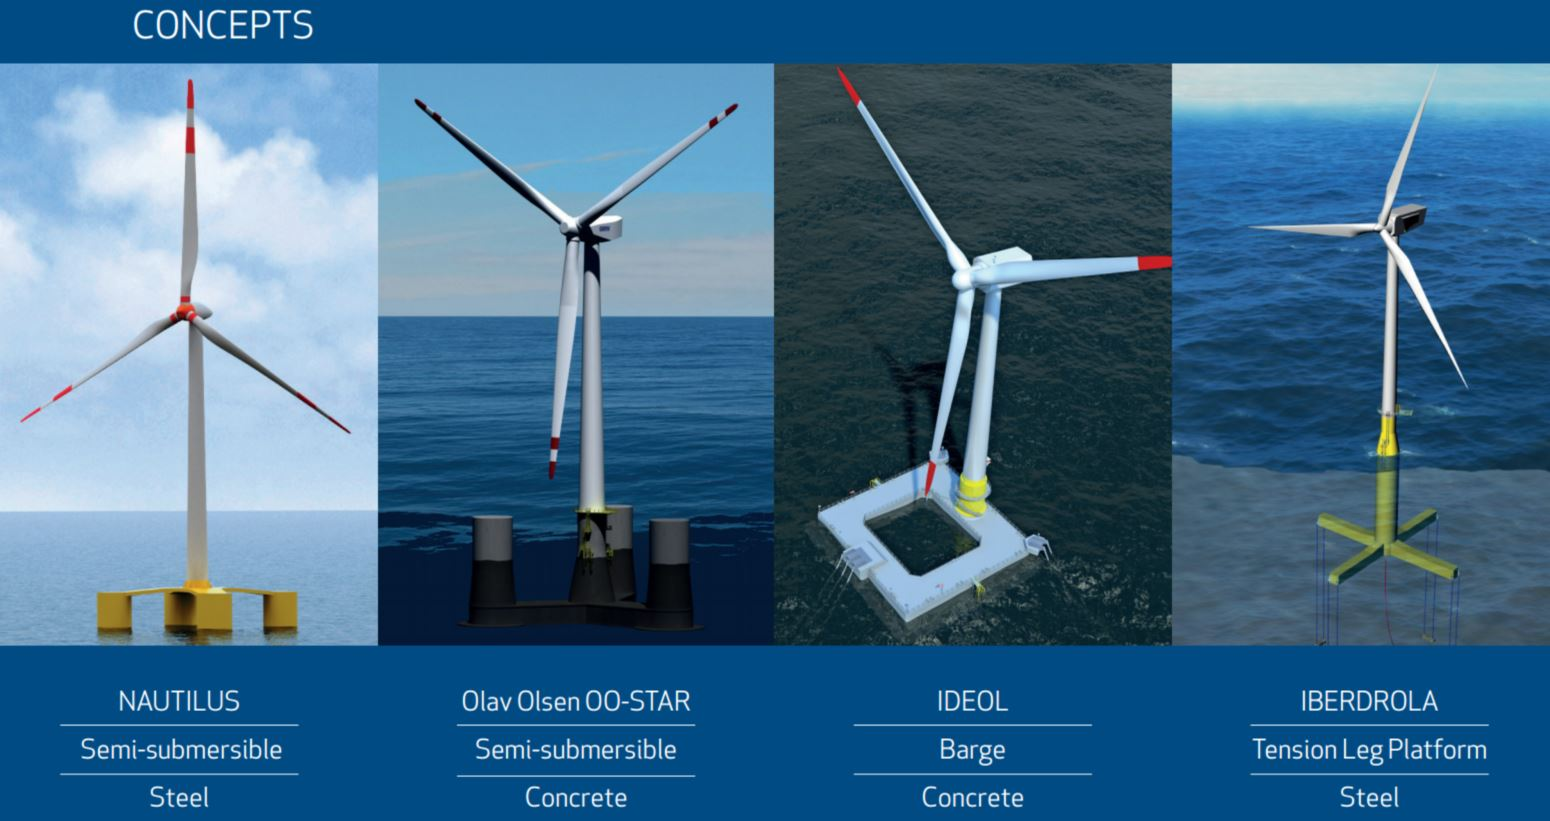
\includegraphics[scale=0.4]{figures/concepts}
\caption[$\; \:$Concepts of the Lifes50+ project]{The different concepts of the Lifes50+ project \cite{Lifes50+} }
 \label{fig:concept}
\end{figure}

\begin{figure}[H]
\centering
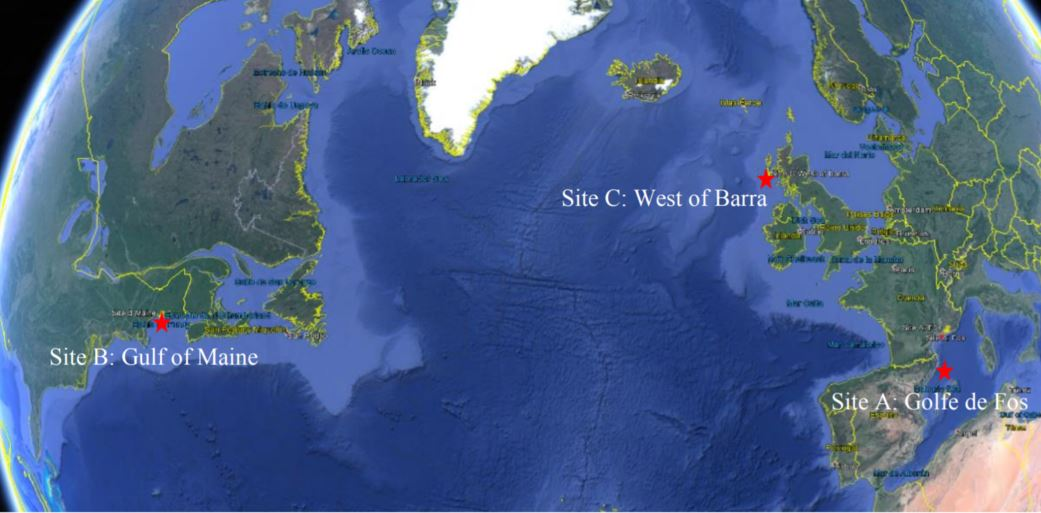
\includegraphics[scale=0.6]{figures/sites}
\caption[$\; \:$Sites for Lifes50+ project]{The different sites for Lifes50+ project \cite{Lifes50+D1.6} }
 \label{fig:sites}
\end{figure}

\subsection{OO-Star}
OO-star is one of the two designs to proceed to the second stage of the project. It is a design developed by the Norwegian company Dr. Techn. Olav Olsen.\newline
\newline
The support structure is a semi-submersible consisting of one column in the center supporting the tower and turbine, and three outer columns equally spaced, all mounted on a star-shaped pontoon, as can be seen in Figure \ref{fig:oostar}

\begin{figure}[H]
\centering
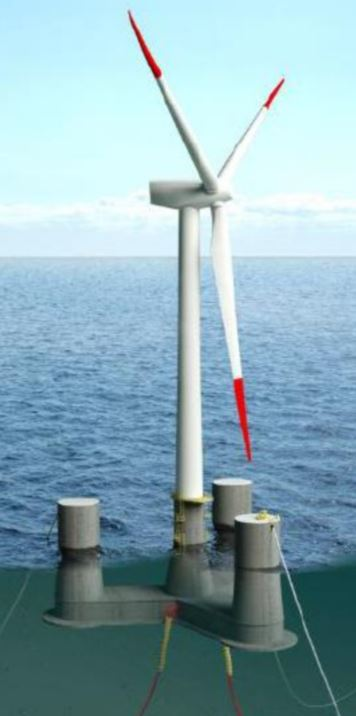
\includegraphics[scale=0.6]{figures/oostar}
\caption[$\; \:$Dr. Techn. Olav Olsen's OO-Star]{Dr. Techn. Olav Olsen's OO-Star \cite{Lifes50+D4.2} }
 \label{fig:oostar}
\end{figure}

\noindent The main material is post-tensioned concrete, and the main dimensions are displayed in Figure \ref{fig:designoostar}

\begin{figure}[H]
\centering
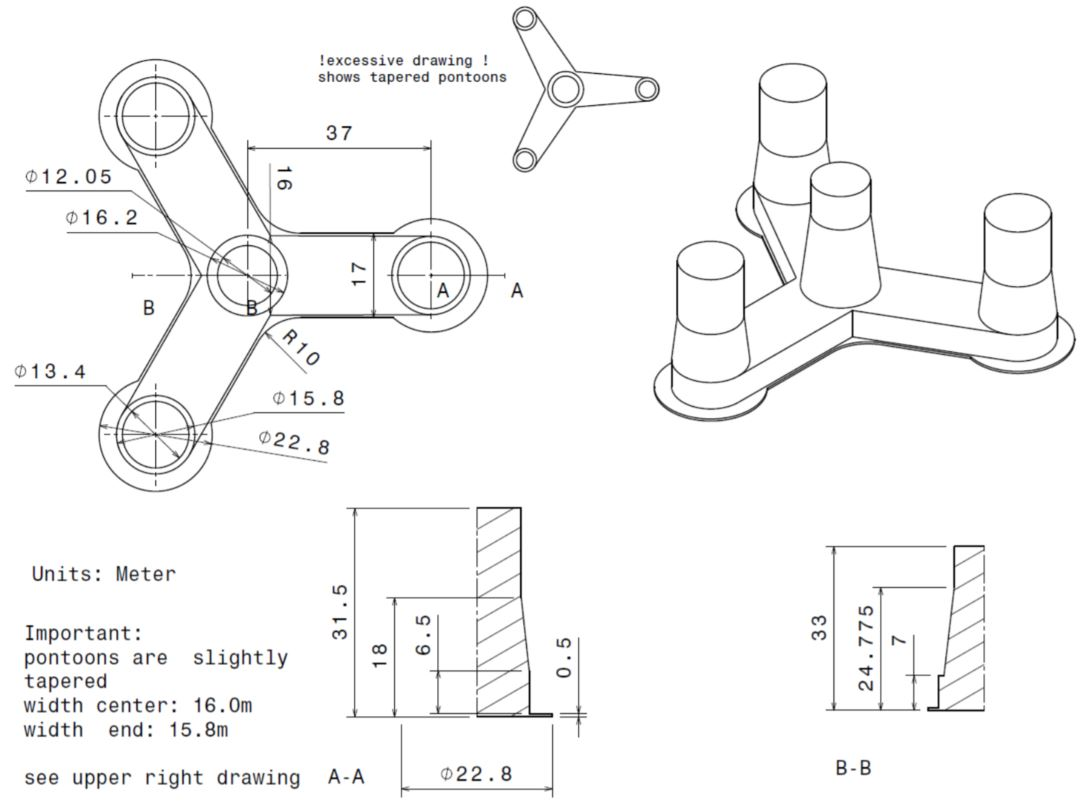
\includegraphics[scale=0.6]{figures/designoostar}
\caption[$\; \:$Main dimensions of OO-Star]{Main dimensions of OO-Star \cite{Lifes50+D4.2} }
 \label{fig:designoostar}
\end{figure}

\section{Environmental Conditions}
As mentioned earlier in this section, 3 possible locations were used for the Lifes50+ project with different degree of challenging conditions. For this project thesis, the chosen location was be West of Barra, Scotland. The main basis for this choice was that this was the site with the deepest water, and this is also the site with the most challenging weather conditions. The exact proposed location is in the area with the coordinates 56.609°N, 7.996°W.  This section contains information mainly from the report \cite{Lifes50+D1.1}.


\begin{figure}[H]
\centering
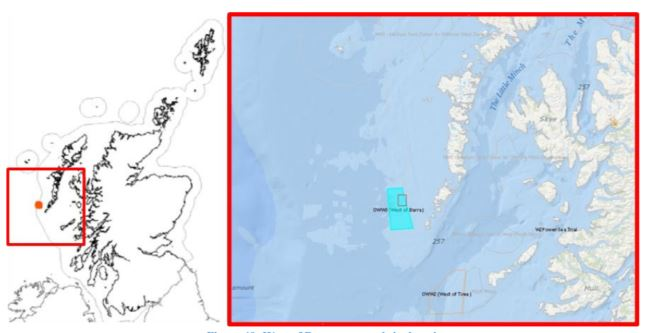
\includegraphics[scale=0.8]{figures/wob}
\caption[$\; \:$West of Barra, Scotland]{Possible location for floating wind turbine, West of Barra, Scotland \cite{Lifes50+D1.1} }
 \label{fig:wob}
\end{figure}

\noindent The water depth at the location West of Barra is between 56-118m. In this project thesis, 118 m was used. 

\subsection{Wind Climate}
\label{sec:windcli}

The wind speeds at West of Barra are high and reliable throughout the year, with a mean annual power density of 1.3 $\frac{kW}{m^2}$. The following wind and wave data is based on \cite{geos2001}, and extrapolated and modified by \cite{Lifes50+D1.1}. 
\\\\
Table \ref{table:wind} shows the ten minute mean wind speed profile at different heights, and extreme value wind speed is shown in Table  \ref{table:windex}
\begin{table} [H]
\centering
\begin{tabular}{ |c|c|}
\hline
 Height [m]& Wind speed [m/s]\\
 \hline
 \hline
 10 & 9.50 \\

 20 & 10.16 \\
 
 50 & 10.97 \\
 
 120 & 11.58 \\

 119 & 11.74  \\
 \hline
\end{tabular}
\caption{Ten minute mean wind speed profile}
\label{table:wind}
\end{table}

\begin{table} [H]
\centering
\begin{tabular}{ |c|c|}
\hline
 Height [m]& Wind speed [m/s]\\
 \hline
 \hline
 10 & 26.47 \\

 20 & 35.63 \\
 
 50 & 44.13 \\
 
 120 & 48.97 \\

 119 & 50.00  \\
 \hline
\end{tabular}
\caption{Ten minute mean extreme value speed profile}
\label{table:windex}
\end{table}

\noindent Figure \ref{fig:scatterwind} shows the scatter diagram for wind conditions at west of Barra. With north being 0 degrees

\begin{figure}[H]
\centering
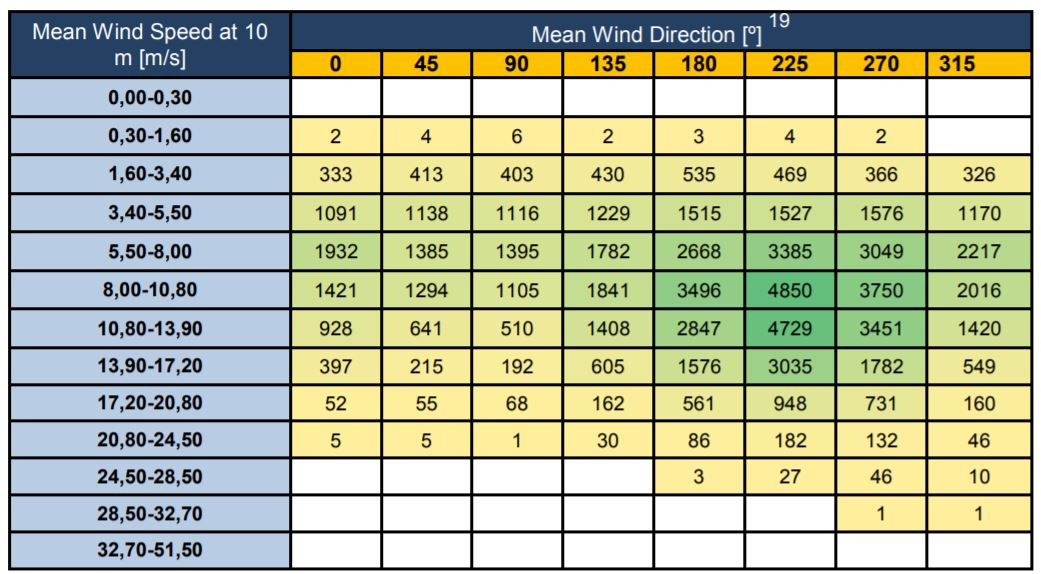
\includegraphics[scale=0.7]{figures/scatterwind}
\caption[$\; \:$Scatter diagram for wind conditions]{Scatter diagram for wind conditions at West of Barra \cite{Lifes50+D1.1} }
 \label{fig:scatterwind}
\end{figure}
 
 \noindent The max annual wind speed at 10 m above sea surface with 1-year return period is calculated in \cite{Lifes50+D1.1} to be  29.36 $\frac{m}{s}$



\subsection{Wave Climate}
The wave loads to be applied to the floating wind turbine are based on the scatter diagram for the location in West of Barra. According to the transfer functions obtained from Dr.Techn.Olav Olsen, severe resonance will occur at periods around 19s-24s in heave. As Tp is only the average of the 1/3 highest waves, resonance was observed for Tps lower than 19s in the global analyses. To avoid the area of severe resonance, an thus extreme response for the wind floater, the sea states for the periods 16 -17, 17-18 seconds and 18-19 seconds were moved to the 15-16 seconds column as can be seen in Figures \ref{fig:scato} and \ref{fig:scatn}, maintaining the total number of observations.

\begin{figure}[H]
\centering
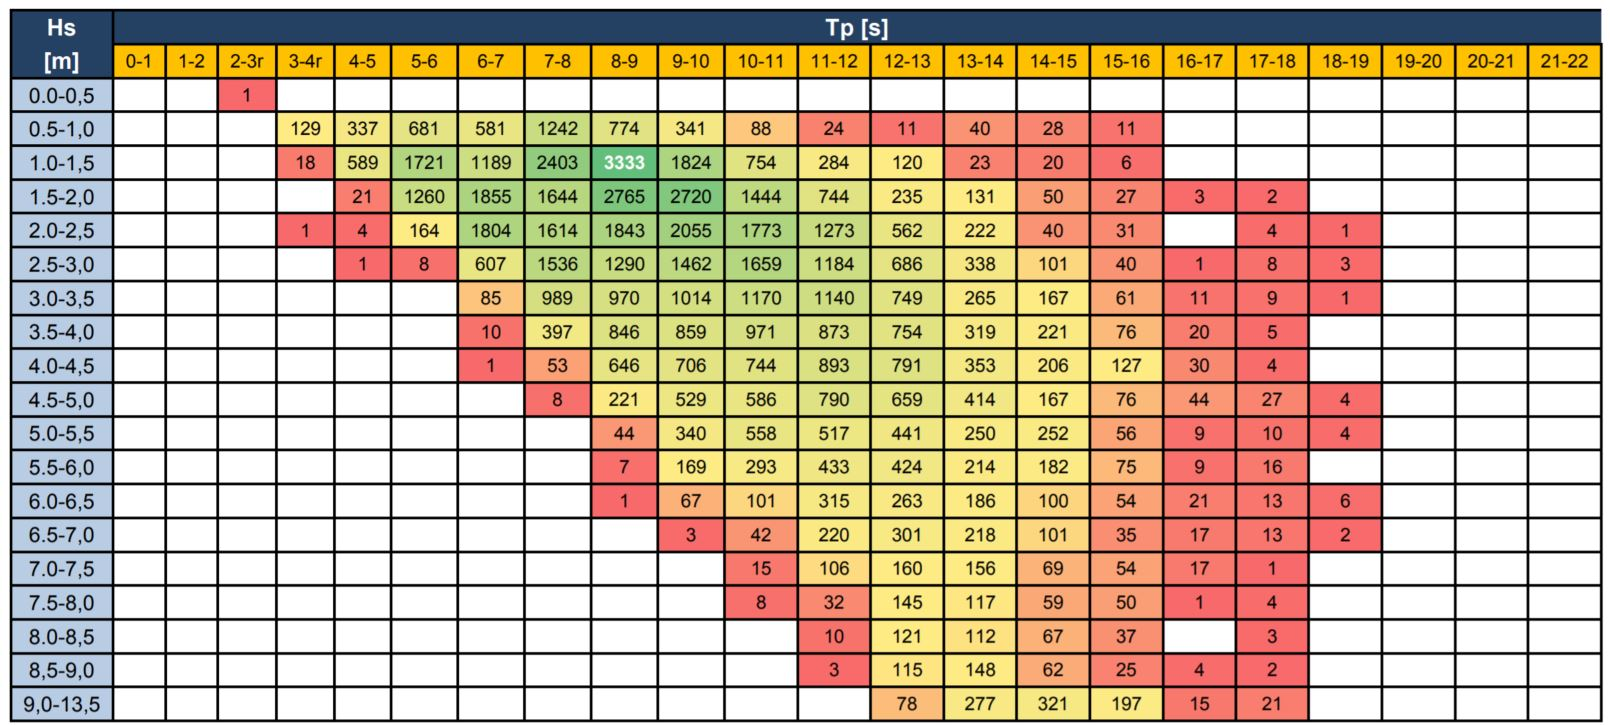
\includegraphics[scale=0.5]{figures/scatteroriginal}
\caption[$\; \:$Original scatter diagram]{Original scatter diagram \cite{Lifes50+D1.1} }
 \label{fig:scato}
\end{figure}

\begin{figure}[H]
\centering
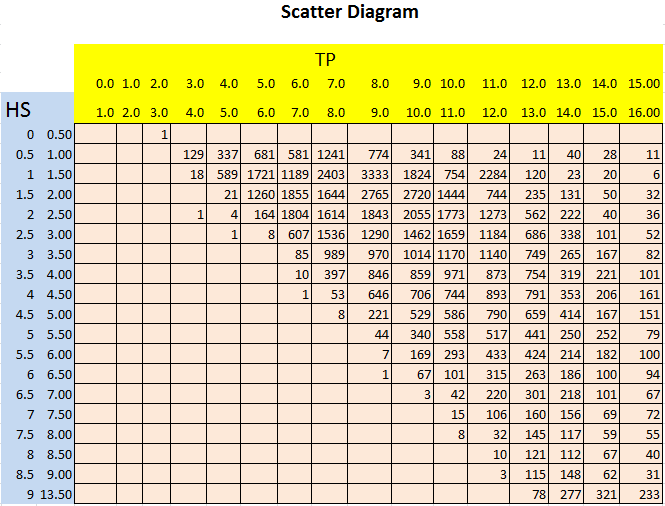
\includegraphics[scale=0.8]{figures/scatternew}
\caption[$\; \:$Modified scatter diagram ]{Modified scatter diagram  }
 \label{fig:scatn}
\end{figure}
 
 \noindent \cite{Lifes50+D1.1} states that there are no data on the correlation between the wind direction and the wave direction.
 \subsection{Current}
 \label{sec:current}
 According to \cite{Lifes50+D1.1}, the coast of Scotland is located on the UK Continental Shelf, so that it is directly affected by the oceanic circulations. However, the amount of water traveling from deep waters of the Atlantic sea to the shallower waters of the continental shelf is reduced due to the steepness of the slope of the shelf. Tidal currents are stronger and easier to predict than the non-tidal currents in the area. Winds, jets and density-driven currents affects the non-tidal currents strongly, and this may lead to large changes of the general current patterns for short periods. There are no specific data on the current conditions of West for Barra. However, according to \cite{dnvenviroment}, when detailed field measurements are missing, the current speed profile can be modelled with two components: wind generated current and tidal current. \newline
  \newline
  \subsubsection{Wind Generated Current}
  The wind induced current speed at still water level (z=0) can be calculated, if no statistical data is available, as:
  
  \begin{equation}
      V_{c,wind}(0)=k U_{1hour,10m}
  \end{equation}
  Where $k$ is a constant in range 0.015-0.03, and $U_{1hour,10m}$ is the 1 hour wind speed at height 10 m above sea level.\newline
  \newline
  By using $k=0.03$ and and 29.36$\frac{m}{s}$ as current speed at still water level (see section \ref{sec:windcli}, the current speed at still water level was calculated to:\newline
\newline
$$V_{c,wind}(0)=0.881$$   
  Then the current speed profile can be calculated as a linear profile from $d_0 < z < 0$:
  
  \begin{equation}
      V_{c,wind}(z)= V_{c,wind}(0) \left( \frac{d_0+z}{d_0}\right)
  \end{equation}
  
  \noindent Where $ V_{c,wind}(z)$ is the current speed at still water level, $d_0$ is the reference depth for wind generated current $d_0$=50m, and z is the distance from still water level, positive upwards. \newline
  \newline
  
\subsubsection{Deep Water Current } 
   The data in this section is taken from \cite{hseenironmental} and reproduced by \cite{Lifes50+D1.1}.\newline
   \newline
   The 50 year return period speed and directions for tidal current and storm surge current was found to be 0.44 m/s in North-East direction and 0.6 m/s in North direction respectively. From this, the 1 year return period velocities could be calculated by multiplying by a correction factor of 0.89. The combined velocity and direction was calculated as the vectorial sum.
   
   
\begin{table} [H]
\centering
\begin{tabular}{ |c|c|c|c|}
\hline
Return Period & Tidal Current & Storm Surge Current & Combined Current \\
 \hline
 \hline
 & Vc[m/s] \hspace{0.3cm} Dir[$^{\circ}$] &  Vc[m/s] \hspace{0.3cm} Dir[$^{\circ}$] & Vc[m/s] \hspace{0.3cm} Dir[$^{\circ}$] \\
 \hline
 1 & 0.39 \hspace{0.7cm} 50 & 0.53 \hspace{0.7cm} 0  & 0,84 \hspace{0.7cm} 21 \\
 50 & 0.44 \hspace{0.7cm} 50 & 0.60 \hspace{0.7cm} 0  & 0,94 \hspace{0.7cm} 21 \\
 \hline
\end{tabular}
\caption{Deep Water Current at Sea Surface, reproduced from \cite{Lifes50+D1.1}}
\label{table:tidcur}
\end{table} 

\noindent According to \cite{dnvenviroment}, the 1 year return period data from Table \ref{table:tidcur} can be used to calculate the tidal and storm surge current profile for $z \leq 0$:

 \begin{equation}
      V_{c,tide}(z)= V_{c,tide}(0) \left( \frac{d+z}{d_0}\right)^{\alpha}
  \end{equation}
  
  \noindent Where $ V_{c,tide}(z)$ is the current speed at still water level, $d$ is the water depth to still water level (taken positive), and z is the distance from still water level, positive upwards, $\alpha$ is the exponent, typically $\alpha = \frac{1}{7}$

   \subsubsection{Current Speed Profile}
  As a simplification, only three different weather conditions are considered: 
  \begin{itemize}
      \item Far: Wind direction and wind induced current direction is the same as wave direction
     \item Neutral: No wind, only tide and storm surge current
     \item Near:  Wind direction and wind induced current direction is the opposite to wave direction
  \end{itemize}
 The current profiles for the three weather conditions were calculated as the vectorial sum of the wind induced current and the tidal- and storm surge current. The profiles are displayed in Table \ref{table:tidcur}, where north is defined as 0 $^{\circ}$:  
\begin{table} [H]
\centering
\begin{tabular}{ |c|c|c|c|}
\hline
Depth [m] & Wind & Tidal and Surge & Total Current Profile \\
 \hline
 \hline
 & Vc[m/s] \hspace{0.3cm} Dir[$^{\circ}$] &  Vc[m/s] \hspace{0.3cm} Dir[$^{\circ}$] & Vc[m/s] \hspace{0.3cm} Dir[$^{\circ}$] \\
 \hline
 0 & 0.881 \hspace{0.7cm} 270 & 1.023 \hspace{0.7cm} 21  & 1.085 \hspace{0.7cm} 331.70 \\
 -10 & 0.705 \hspace{0.7cm} 270 & 1.008 \hspace{0.7cm} 21  & 1.010 \hspace{0.7cm} 340.49 \\
 -20 & 0.528 \hspace{0.7cm} 270 & 0.992 \hspace{0.7cm} 21  & 0.942
 \hspace{0.7cm} 349.47 \\
 -30 & 0.352 \hspace{0.7cm} 270 & 0.973 \hspace{0.7cm} 21  & 0.908 \hspace{0.7cm} 364.79 \\
 -40 & 0.176 \hspace{0.7cm} 270 & 0.952 \hspace{0.7cm} 21  & 0.904 \hspace{0.7cm} 10.48 \\
 -50 & 0.0 \hspace{0.7cm} - & 0.928 \hspace{0.7cm} 21  & 0.928 \hspace{1.15cm} 21 \\
  -60 & 0.0 \hspace{0.7cm} - & 0.900 \hspace{0.7cm} 21  & 0.900 \hspace{1.15cm} 21 \\
 -70 & 0.0 \hspace{0.7cm} - & 0.864 \hspace{0.7cm} 21  & 0.864 \hspace{1.15cm} 21 \\
  -80 & 0.0 \hspace{0.7cm} - & 0.817 \hspace{0.7cm} 21  & 0.817 \hspace{1.15cm} 21 \\
 -90 & 0.0 \hspace{0.7cm} - & 0.741 \hspace{0.7cm} 21  & 0.741 \hspace{1.15cm} 21 \\ 
 -100 & 0.0 \hspace{0.7cm} - & 0.0 \hspace{0.7cm} -  & 0.0 \hspace{1.15cm} - \\ 
 \hline
\end{tabular}
\caption{Current Speed and Direction Profile for Near wind condition, partly from \cite{Lifes50+D1.1}}
\label{table:tidcur}
\end{table}   

\begin{table} [H]
\centering
\begin{tabular}{ |c|c|c|c|}
\hline
Depth [m] & Wind & Tidal and Surge & Total Current Profile \\
 \hline
 \hline
 & Vc[m/s] \hspace{0.3cm} Dir[$^{\circ}$] &  Vc[m/s] \hspace{0.3cm} Dir[$^{\circ}$] & Vc[m/s] \hspace{0.3cm} Dir[$^{\circ}$] \\
 \hline
 0 & 0.0 \hspace{0.7cm} - & 1.023 \hspace{0.7cm} 21  & 1.023 \hspace{0.7cm} 21 \\
 -10 & 0.0 \hspace{0.7cm} - & 1.008 \hspace{0.7cm} 21  & 1.008 \hspace{0.7cm} 21 \\
 -20 & 0.0 \hspace{0.7cm} - & 0.992 \hspace{0.7cm} 21  & 0.992
 \hspace{0.7cm} 21 \\
 -30 & 0.0 \hspace{0.7cm} - & 0.973 \hspace{0.7cm} 21  & 0.973 \hspace{0.7cm} 21 \\
 -40 & 0.0 \hspace{0.7cm} - & 0.952 \hspace{0.7cm} 21  & 0.952 \hspace{0.7cm} 21 \\
 -50 & 0.0 \hspace{0.7cm} - & 0.928 \hspace{0.7cm} 21  & 0.928 \hspace{1.15cm} 21 \\
  -60 & 0.0 \hspace{0.7cm} - & 0.900 \hspace{0.7cm} 21  & 0.900 \hspace{1.15cm} 21 \\
 -70 & 0.0 \hspace{0.7cm} - & 0.864 \hspace{0.7cm} 21  & 0.864 \hspace{1.15cm} 21 \\
  -80 & 0.0 \hspace{0.7cm} - & 0.817 \hspace{0.7cm} 21  & 0.817 \hspace{1.15cm} 21 \\
 -90 & 0.0 \hspace{0.7cm} - & 0.741 \hspace{0.7cm} 21  & 0.741 \hspace{1.15cm} 21 \\ 
 -100 & 0.0 \hspace{0.7cm} - & 0.0 \hspace{0.7cm} -  & 0.0 \hspace{1.15cm} - \\ 
 \hline
\end{tabular}
\caption{Current Speed and Direction Profile for Neutral wind condition, partly from \cite{Lifes50+D1.1}}
\label{table:tidcur}
\end{table}   

\begin{table} [H]
\centering
\begin{tabular}{ |c|c|c|c|}
\hline
Depth [m] & Wind & Tidal and Surge & Total Current Profile \\
 \hline
 \hline
 & Vc[m/s] \hspace{0.3cm} Dir[$^{\circ}$] &  Vc[m/s] \hspace{0.3cm} Dir[$^{\circ}$] & Vc[m/s] \hspace{0.3cm} Dir[$^{\circ}$] \\
 \hline
 0 & 0.881 \hspace{0.7cm} 90 & 1.023 \hspace{0.7cm} 21  & 1.571 \hspace{0.7cm} 52.56 \\
 -10 & 0.705 \hspace{0.7cm} 90 & 1.008 \hspace{0.7cm} 21  & 1.421 \hspace{0.7cm} 48.57 \\
 -20 & 0.528 \hspace{0.7cm} 90 & 0.992 \hspace{0.7cm} 21  & 1.279
 \hspace{0.7cm} 43.65 \\
 -30 & 0.352 \hspace{0.7cm} 90 & 0.973 \hspace{0.7cm} 21  & 1.147 \hspace{0.7cm} 37.64 \\
 -40 & 0.176 \hspace{0.7cm} 90 & 0.952 \hspace{0.7cm} 21  & 1.029 \hspace{0.7cm} 30.19 \\
 -50 & 0.0 \hspace{0.7cm} - & 0.928 \hspace{0.7cm} 21  & 0.928 \hspace{1.15cm} 21 \\
  -60 & 0.0 \hspace{0.7cm} - & 0.900 \hspace{0.7cm} 21  & 0.900 \hspace{1.15cm} 21 \\
 -70 & 0.0 \hspace{0.7cm} - & 0.864 \hspace{0.7cm} 21  & 0.864 \hspace{1.15cm} 21 \\
  -80 & 0.0 \hspace{0.7cm} - & 0.817 \hspace{0.7cm} 21  & 0.817 \hspace{1.15cm} 21 \\
 -90 & 0.0 \hspace{0.7cm} - & 0.741 \hspace{0.7cm} 21  & 0.741 \hspace{1.15cm} 21 \\ 
 -100 & 0.0 \hspace{0.7cm} - & 0.0 \hspace{0.7cm} -  & 0.0 \hspace{1.15cm} - \\ 
 \hline
\end{tabular}
\caption{Current Speed and Direction Profile for Far wind condition, partly from \cite{Lifes50+D1.1}}
\label{table:tidcur}
\end{table}   

\section{Wind Turbine Floater Motions}
To simulate the motion of OO-Star, Dr. Techn. Olav Olsen have provided the transfer functions for all 6 degrees of freedom of the vessel. The transfer functions are valid for the center of the model, however, the cable is attached some distance from the center of gravity as can be seen in Figure \ref{fig:cabhang}. This distance has been calculated to be 9.24m, and had to be taken into consideration. 

\begin{figure}[H]
\centering
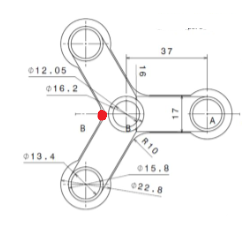
\includegraphics[scale=1.2]{figures/cabhang}
\caption[$\; \:$Cable hang off position]{Cable hang off position, modified from \cite{Lifes50+D4.2}}
 \label{fig:cabhang}
\end{figure}
 \noindent The transfer functions of OO-star are confidential and can not be reproduced in this report. 
 
\section{Power Cable}
The choice of power cable cross section is based on guidance from Professor Svein Sævik. 

\subsection{Cable Cross Section}
 An illustration of the model cross section used is shown in Figure \ref{fig:cross2}. 

\begin{figure}[H]
\centering
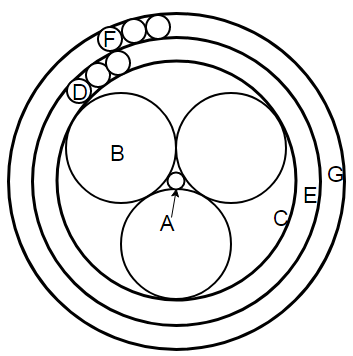
\includegraphics[scale=0.6]{figures/cross2}
\caption[$\; \:$Cable cross section in local model]{Illustration of cable cross section in local model  }
 \label{fig:cross2}
\end{figure}

\noindent The different components in the local model are:
\begin{enumerate}[label=\Alph*]
\item Core
\item Electrical conductor + insulation
\item Sheath around conductors
\item 1st layer of Armouring 
\item Tape between the two layers of armouring
\item 2nd layer of armouring
\item Protective sheath
\end{enumerate}

\noindent The dimensions of components of the cross-section are based on the conductor + insulation cross-section, and all other dimensions are calculated from this. The conductor itself has an area of 95$mm^2$, and in addition, there is a layer of insulation, making the radius of the of conductor + insulation 15mm.  The calculations of the radius of the core and the 1st sheath are based on trigonometry. By imagining a like-sided triangle with its corners in the center of each of the conductors, the following relations can be derived: 


  \begin{equation}
   r_{ct} = r_c (\tan(60)-\tan(30)-1)
\end{equation}

 \noindent Where $r_{ct}$ is the radius of the core and $r_c$ is the radius of the conductor.

 \begin{equation}
   r_{s} = r_c (1+\tan(60)-\tan(30))
\end{equation}
 
  \noindent Where $r_{s}$ is the radius of the sheath around the conductors and $r_c$ is the radius of the conductor. \newline
  \newline 
  \noindent The dimensions of the local model are given in Table \ref{table:dim}, and are determined in agreement with Professor Svein Sævik. . 


\begin{table} [H]
\centering
\begin{tabular}{ |c|c|c|}
\hline
Component & Radius [mm] & Thickness [mm] \\
 \hline
 \hline
 Conductor + Insulation & 15 &\\

 Center tube & 2.32& \\
 
 Sheath 1 & 33.07 & 1.5 \\
 
Armouring & 1.5 &  \\

Tape & 37.57 & 0.5 \\

Sheath 3 & 42.82& 3  \\

 \hline
\end{tabular}
\caption{Dimensions of local model}
\label{table:dim}
\end{table} 

\noindent There are 66 steel armouring fibers in the inner layer of the armouring, and 74 in the outer layer. This is calculated by the following expression:
\begin{equation}
    n_i=\frac{F_j\cos(\alpha)\pi D_c}{D_s}
\end{equation}
Where $F_j$ is the fill factor (0.9 was used), $\alpha$ is the lay angle (8 degrees was used), $D_c$ is the diameter of the cable and $D_s$ is the diameter of one steel fibre. 
\subsection{Power Cable SN fatigue data}
To estimate the life time of the power cable, a S-N curve in Figure \ref{fig:snplot} was used. 

\begin{figure}[H]
\centering
\includegraphics[scale=0.6]{figures/SNplot}
\caption[$\; \:$S-N data]{S-N data for case scenario,\cite{savik2014} }
 \label{fig:snplot}
\end{figure}
\noindent The S-N curve follows the log linear relationship of equation \ref{eq:sn}, with m=8.424 and c=2.88e25 according to \cite{Nasution2013}
\chapter{Numeric Models}
\label{chap:numeric}
In this chapter, the numeric theory behind the two models used to analyze the fatigue of the dynamic power cable will be presented.

\section{The Finite Element Method}
The finite element method is a numerical procedure for solving differential equations, and is often used in analysis of structures. The finite element method will give an approximate solution, with increasing accuracy with decreasing mesh size. According to the Finite Element Theory, for a static linear system, the system relationship will be:
\begin{equation}
    \boldsymbol{R}= \boldsymbol{K}\boldsymbol{r}
\end{equation}
Where R is the global load matrix, K is the global stiffness matrix, and r is the nodal displacement vector.\newline
\newline
This is based on the following principles:
\begin{itemize}
    \item Equilibrium
    \item Kinematic compatibility
    \item Stress-strain relationship
\end{itemize}
 \cite{moan2003}
\subsection{Principle of Virtual Work}
The element stiffness relationship can be derived based on virtual work (Galerkin's Method). This method assumes a displacement for each element so that the displacement is continuous between elements. The method can be generalized and used for all kinds of structural problems in all dimensions, \cite{moan2003}. The method gives an approximation rather than the exact solution. This is done by,  in average, fulfilling the differential equations in the problem. By setting the internal work equal to the external work, it is assumed that the error from assuming the weight function in the external work is equal to the error in the internal work. If the weight functions are selected so that the boundary conditions are fulfilled appropriately, the error in the external work will cancel out. This means that the total error in the volume integration is zero in average, but at an arbitrary point, the equilibrium equation is not necessarily fulfilled. This is referred to as integrated equilibrium. The principle of virtual work in a body with deformed volume and surfaces in equilibrium:   

\begin{equation}
    \int_v (\rho \boldsymbol{\ddot{u}} - \boldsymbol{f}) \cdot \delta \boldsymbol{u}dV + \int_V \boldsymbol{\sigma}: \delta \epsilon dV - \int_S \boldsymbol{t} \cdot \delta \boldsymbol{u} dS =0
    \label{eq:virtual}
\end{equation}
Where V refers to the volume, $\rho$ is the material density, $ \boldsymbol{\ddot{u}}$ is the acceleration field, $ \boldsymbol{f}$ is the volume force vector, $\delta$ is the virtual displacement,  $\boldsymbol{\sigma}$ is the stress tensor, $\epsilon$ is the natural strain tensor, $\boldsymbol{t}$ is the surface traction, $\boldsymbol{u}$ is the displacement vector and S refers to the surface \cite{Bflextheory2013}. 

\begin{comment}
In BFLEX and SIMA RIFLEX(?) the stress tensor is given as: 
\begin{equation}
\boldsymbol{S}=\frac{\rho_0}{\rho} \boldsymbol{F^{-1}} \cdot \boldsymbol{\sigma} \cdot \boldsymbol{F}
\end{equation}
Where $\rho_0$ is the density of the material in the initial configuration, and $\rho$ is the density of the material in the deformed configuration, $\boldsymbol{F}$ is the deformed gradient. In this case, strains are usually small so that $\boldsymbol{S}$ and $\boldsymbol{\sigma}$ can be treated equally. However, equation \ref{eq:virtual} need to be modified as change of are will affect pressure loads. The equation then becomes:

\begin{equation}
    \int_v (\rho \boldsymbol{\ddot{u}} - \boldsymbol{f}) \cdot \delta \boldsymbol{u}dV_0 + \int_V \boldsymbol{\sigma}: \delta \epsilon dV_0 - \int_S \boldsymbol{t} \cdot \delta \boldsymbol{u} dS_0 -  \int_S \boldsymbol{p} \cdot \delta \boldsymbol{u}(1+\epsilon_{11} + \epsilon_{33})  dS_0 =0
    \label{eq:virtual2}
\end{equation}
Where $\epsilon_{11}$ and $\epsilon_{33}$ are principle strains of surface plane.
\end{comment}
\section{Method for Static calculation}
\subsection{Static Non-linear Theory}
According to \cite{moan2003}, a system is non-linear if it contains non-linear material, large displacements or geometry non-linearity. For non-linear problems, the stiffness will depend on the displacement:
\begin{equation}
    \boldsymbol{R}=\boldsymbol{K(r)}\boldsymbol{r}
\end{equation}
The stiffness matrix is often written on differential form, with the incremental stiffness matrix, $K_I$:
\begin{equation}
    d\boldsymbol{R}=\frac{d}{d\boldsymbol{r}}(\boldsymbol{K(r)r})d\boldsymbol{r}
\end{equation}
\begin{equation}
  d\boldsymbol{R}= \boldsymbol{K_I(r)}d\boldsymbol{r}
  \label{eq:system}
\end{equation}
In general it can be challenging to determine $\boldsymbol{r}$ for a given $\boldsymbol{R}$ analytically, and thus iterative methods will have to be used. Only the methods relevant for this Master Thesis will be presented here. 

\subsection{Combined Method}
The combined method is a combination of the Euler-Cauchy Method and the Newton-Raphson Method. 
\subsubsection{Euler-Cauchy Method}
This method it an incremental method, meaning that the external load is applied step-wise. For each step the displacement increment $\boldsymbol{\Delta r}$ is determined. The total displacement is then calculated by adding the incremental displacements. The incremental stiffness matrix $\boldsymbol{K_I}$ is constant for each increment, and is calculated for each step based on the current displacement and stress before a new load increment is added. This is illustrated in Figure \ref{fig:euler}. For load increment number (m+1):
\begin{equation}
\Delta \boldsymbol{r_{m+1}}= \boldsymbol{K_{I}}(\boldsymbol{r_{m}})^{-1} \Delta \boldsymbol{R_{m+1}}
\end{equation}
\newline 
\newline
where:
\begin{equation}
    \Delta \boldsymbol{R_{m+1}} = \boldsymbol{R_{m+1}} - \boldsymbol{R_{m}}
\end{equation}
\begin{equation}
    \boldsymbol{r_{m+1}}=\boldsymbol{r_{m}}+\Delta \boldsymbol{r_{m+1}}
\end{equation}

\begin{figure}[H]
\centering
\includegraphics[scale=1]{figures/euler}
\caption[$\; \:$Euler-Cauchy Method]{Euler-Cauchy Method  \cite{moan2003} }
 \label{fig:euler}
\end{figure}
\noindent As the incremental stiffness from the previous increment is used, this will only give an approximation, and does not fulfill total equilibrium. This can be seen in Figure \ref{fig:euler} where the approximation is plotted with the true solution. More accurate results will be obtained by using smaller increment size and by equilibrium corrections. 
\subsubsection{Newton Raphson Method}
\label{sec:newton}
The Newton-Raphson Method is an iterative method, and is based on the Newton-Raphson Algorithm:
\begin{equation}
    x_{n+1}=x_n - \frac{f(x_n)}{f'(x_n)}
\end{equation}
 Where $f'(x_n)$ is the derivative of $f(x)$ at $x=x_n$. This is illustrated in Figure \ref{fig:newton}
 \noindent This algorithm can be generalized to solve the non-linear system equation \ref{eq:system}:
 \begin{equation}
  \boldsymbol{r_{n+1}}= \boldsymbol{r_n-K_I^{-1}(r_n)(R_{int}-R)} 
\end{equation}
This method requires that $\Delta r_{n+1}$ is solved for from 
\begin{equation}
   \boldsymbol{R-R_{int}}=\boldsymbol{K_{I(n)}\Delta r_{n+1}}
   \label{eq:newton}
\end{equation}
and that $K_I$ is established. 
 \begin{figure}[H]
\centering
\includegraphics[scale=0.5]{figures/newton2}
\caption[$\; \:$Newton-Raphson Iteration]{Newton-Raphson Iteration \cite{moan2003} }
 \label{fig:newton}
\end{figure}
\noindent Newton-Raphson method is time consuming, but calculation time can be improved by updating $\boldsymbol{K_I}$ less frequently. That is called the modified Newton-Raphson method, and usually gives slower convergence.  The iteration ends when the displacement from one iteration to the next is smaller than the convergence criteria:
\begin{equation}
    ||\boldsymbol{r_{n+1}-r_n||} < \epsilon
\end{equation}

\subsubsection{Combined Method}
\label{sec:combined}
When combining the two methods load is applied according to the Euler-Cauchy method, and iteration until equilibrium is done according to the modified Newton-Raphson method for each increment. This is illustrated in Figure \ref{fig:combined} The method is considered to be effective as long as the load curve is increasing with displacement. For extremal points in the load-displacement curve, extra procedures need to be implemented.    

 \begin{figure}[H]
\centering
\includegraphics[scale=0.8]{figures/combined}
\caption[$\; \:$Combined Method]{Combined Method \cite{moan2003} }
 \label{fig:combined}
\end{figure}
\section{Method for Dynamic Calculation}
Dynamic analysis has to be considered when external loads are not applied in a very slow manner. Dynamic loads are different from static loads by implying a time dependent solution and by introducing inertia loads throughout the structure, and often also damping. The equilibrium equation for a dynamic system is stated by \cite{Langen1999} as:

\begin{equation}
  \boldsymbol{M \ddot{r}} + \boldsymbol{C \dot{r}} + \boldsymbol{Kr} =  \boldsymbol{Q}(t)
  \label{eq:eq}
\end{equation}

\noindent A variation of equation \ref{eq:eq} is the semi-discrete global equation describing the instantaneous equation of motion of a nonlinear system at time t. This relation is presented by \cite{Mathisen1990} as:
\begin{equation}
    \boldsymbol{R^I}+ \boldsymbol{R^D} + \boldsymbol{R^S}=\boldsymbol{R^E}
\end{equation}
Where $\boldsymbol{R^I}$ is the inertia force vector, $\boldsymbol{R^D}$ is the damping force vector, $\boldsymbol{R^S}$ is the internal force vector and $\boldsymbol{R^E}$ is the external force vector. \newline
\newline
The inertia forces relate to the mass matrix as:
\begin{equation}
    \boldsymbol{R^I}= \boldsymbol{R^I(\ddot{r},\dot{r},r,}t)=\boldsymbol{M(\ddot{r},\dot{r},r,}t)\boldsymbol{r}
\end{equation}

\noindent The internal forces $\boldsymbol{R^S}$ can be established by:
\begin{equation}
    \frac{\partial \boldsymbol{R^S} }{\partial\boldsymbol{r}}= \boldsymbol{K^M}+\boldsymbol{K^G}
\end{equation}
\noindent The total tangential stiffness is now:
\begin{equation}
    \boldsymbol{K^_T}=\boldsymbol{K_T(\ddot{r},\dot{r},r},t)=\boldsymbol{K^M}+\boldsymbol{K^G}+\boldsymbol{K^{NC}}
\end{equation}
\begin{equation}
    \boldsymbol{K^{NC}}=\boldsymbol{K^{NC}(\ddot{r},\dot{r},r},t)=  \frac{\partial \boldsymbol{R^{NC}} }{\partial\boldsymbol{r}}
\end{equation}
\noindent Where $\boldsymbol{K^M}$ and $\boldsymbol{K^G}$ are the material and geometric stiffness matrices respectively, and $\boldsymbol{K^{NC}}$ is the total external non-conservative external forces. \newline
\newline
The equivalent damping force can be expressed as:
\begin{equation}
    \boldsymbol{R^_D}=\boldsymbol{R_D(\ddot{r},\dot{r},r},t)=  \boldsymbol{C_T}\boldsymbol{\dot{r}}
\end{equation}
And the tangential damping matrix is:
\begin{equation}
      \boldsymbol{C_{T}}=\boldsymbol{C_T(\ddot{r},\dot{r},r,}t)=\alpha_1 \boldsymbol{M}+\alpha_2\boldsymbol{K_T} + C_d 
\end{equation}
Where $\alpha_1$ and $\alpha_2$ are the damping coefficients for the Rayleigh damping and $C_d$ is the damping coefficient matrix for additional discrete nodal points.  
\noindent
\newline
\newline 
\noindent  The dynamic equilibrium equation is an initial value problem, meaning that the solution is determined by start values. Practical numerical integration methods use a step-by-step approach, where the time interval is divided into sub-intervals with step length h. Displacement, velocity, and acceleration are known for the beginning of the sub-interval, and the solution for the end of the sub-interval is calculated by assuming the variation of the acceleration over the time step. The computed value will be used to determine the velocity and displacement across the time step, and they will be the start values for the next sub-interval. This way, an approximated solution is calculated at instants along the time axis, and accuracy increases as h decreases, \cite{Langen1999}.
\newline 
\newline
 \noindent How the acceleration changes during a time step is suggested by several methods, and can be explicit or implicit. A nonlinear implicit method requires iteration at each time step to establish for each time step, while this is not necessary for an explicit method. Only the methods relevant to this master thesis will be presented\newline
 \newline
\noindent 
\subsection{Newmark's $\boldsymbol{\beta}$ Family}
\label{sec:newmark}
Newmark-$\boldsymbol{\beta}$ is a family of numerical integration of the dynamic equilibrium equations. It can easily be derived from assuming constant average acceleration over the time step. The following equations are taken from \cite{sintef2017} and \cite{Mathisen1990}: 
\begin{equation}
   \boldsymbol{M_t \ddot{r}_{t+\Delta t}} + \boldsymbol{C_{T,t}\dot{r}_{t+\Delta t}} + \boldsymbol{R_{t+\Delta t}^S}=\boldsymbol{{R_{t+\Delta t}^E}}
   \label{eq:new}
\end{equation}
\begin{equation}
    \boldsymbol{\dot{r}_{t+\Delta t}} =\boldsymbol{\dot{r}_{t}}+(1-\gamma)\boldsymbol{\ddot{r}_{t}}\Delta \tau + \gamma \boldsymbol{\ddot{r}_{t+\Delta t}} \Delta \tau
\end{equation}
\begin{equation}
    \boldsymbol{r_{t+\Delta t}} =\boldsymbol{r_{t}}\Delta \tau + (\frac{1}{2}-\beta)\boldsymbol{\ddot{r}_{t}}(\Delta \tau)^2 + \beta \boldsymbol{\ddot{r}_{t+\Delta t}} (\Delta \tau)^2
\end{equation}
where  $\Delta \tau =\theta \Delta t, \leq 1.0$\newline
\newline
$\gamma$ and $\beta$ are parameters defining the change in acceleration, velocity and displacement vectors in time step $\Delta t$. \cite{Langen1999} explains that the equations are obtained from Taylor-series expansion.  Different values of these parameters give different methods in the Newmark-$\boldsymbol{\beta}$ family. $\gamma$ represents the numerical damping, taken from \cite{sintef2017}: 
\begin{itemize}
    \item $\gamma > \frac{1}{2}$: Positive numerical damping
    \item $\gamma < \frac{1}{2}$: Negative numerical damping
    \item $\gamma = \frac{1}{2}$: No numerical damping
\end{itemize}

\noindent $\gamma = \frac{1}{2}$ is normally used to assure second order accuracy and stability. 
According to \cite{Mathisen1990}, the Newmark-$\boldsymbol{\beta}$ method may have difficulties with solving non-linear problems if they are not discretized in the right way. \newline
\newline
\noindent In dynamic analysis, the higher modes are of little interest, and these can be removed by introducing increased damping ratio. The Newmark's $\boldsymbol{\beta}$ Family will remove the medium modes, and not affecting the lowest and highest modes. The higher modes can be removed by introducing numerical damping, but it is at the cost of accuracy.  The method can be applied both for linear and non-linear analysis \cite{sintef2017}.

\subsection{Modified Hilber-Hughes-Taylor Method}
\label{sec:HHT}
The problem with accuracy when removing the higher modes can be fixed by using Hilber-Hughes-Taylor Method, often referred to as HHT-$\alpha$. The method maintains accuracy while introducing artificial damping of the higher modes. This is done through modification of equation \ref{eq:new}. 
\begin{equation}
   \boldsymbol{M_t \ddot{r}_{t+\Delta t}} + (1+\alpha_H)\boldsymbol{C_{T,t}\dot{r}_{t+\Delta t}}  -\alpha_H\boldsymbol{C_{T,t}\dot{r}}_{n}+ (1+\alpha_H)\boldsymbol{R_{t+\Delta t}^S}-\alpha_H\boldsymbol{R_{t}^S}=(1+\alpha_H) \boldsymbol{R_{t+\Delta t}^E}-\alpha_H\boldsymbol{R_{t}^E}
\end{equation}

The method is unconditionally stable when:
\begin{itemize}
    \item $-\frac{1}{3} \leq \alpha_H \leq 0 $
    \item  $\gamma = \frac{1}{2} (1-2 \alpha_H)$
    \item  $\beta = \frac{1}{4} (1- \alpha_H)^2$
\end{itemize}

\noindent The method is effectively suppressing high frequency and also retains second-order accuracy. \cite{Mathisen1990}

\section{Global Model in SIMA RIFLEX}
SIMA RIFLEX is a computer program made for analyzing slender structures such as flexible risers and mooring lines developed by SINTEF Ocean. The Combined Method is used for the static calculation and Newmark-$\boldsymbol{\beta}$ is used for dynamic analysis. These methods are described in section \ref{sec:combined} and \ref{sec:newmark} respectively. 


\subsection{Element Formulation}
\label{sec:ghost}
SIMA RIFLEX uses co-rotated ghost reference as element formulation for beam elements. 
\begin{comment}
\subsection{Total Lagrangian Formulation}
\label{sec:ghost}
For non-linear analysis, an incremental approach is necessary as described above. According to \cite{sintef2017}, the initial configuration of the body, C0, and the deformed Cn at time t, and then the new incremental deformation Cn+1 at t+$\Delta$t. Cn+1 will be similar to Cn, as $\Delta$t is small. This formulation where the strains in all the incremental configurations are referred to the initial configuration is called "Total Lagrangian Formulation". \cite{Mathisen1990} states that this method can produce false straining in beam elements when exposed to large rotations, and should thus only be used for small rotations
\subsubsection{Co-Rotated Ghost Reference}
\label{sec:ghost}
\end{comment}
Co-rotated beam elements use Green strain and 2nd
Piola-Kirchhoff stresses as the Total Lagrangian formulation, but adapts the procedure of Updated Lagrange formulation where the configuration is updated. This yields the following stiffness matrix:
\begin{equation}
    \boldsymbol{K_I}= \boldsymbol{K_0} + \boldsymbol{K_\sigma}
\end{equation}
This is convenient when it is assumed that the initial configuration deforms as a rigid body, and will move and rotate with the motion of the body. At any time the initial configuration is close to the deformed configuration \cite{sintef2017}. \cite{Mathisen1990} explains that each beam element has a local coordinate system, $i_i^0$. This is illustrated in Figure \ref{fig:coro} where the initial configuration $C_0$ moves as a rigid body with the element and becomes $C_{0n}$. The deformed beam element will have its local coordinate system rotated, now denoted $i_ia$ and $i_i^b$. This forms the reference for calculation of stresses and strains. 

\begin{figure}[H]
\centering
\includegraphics[scale=0.5]{figures/coro}
\caption[$\; \:$Co-rotated Ghost Reference]{Co-rotated Ghost Reference \cite{Mathisen1990} }
 \label{fig:coro}
\end{figure}

\subsection{Element Description}
In this section, the relevant element type and its kinematics will be presented. Only  the element that will be used in the project/master thesis is included. 
\subsubsection{Beam element}
\noindent The beam element in SIMA RIFLEX has 2 nodes with 6 degrees of freedom for each node, 3 translational and 3 rotational that can be seen in Figure \ref{fig:beamri} that are defined in relation to the local Cartesian coordinate system in the initial C0n configuration,
\cite{sintef2017}.

\begin{figure}[H]
\centering
\includegraphics[scale=0.5]{figures/beamri}
\caption[$\; \:$Beam Element]{Degrees of freedom for beam element\cite{sintef2017} }
 \label{fig:beamri}
\end{figure}

\noindent \cite{sintef2017} states that it is assumed that straight lines normal to the midplane will remain straight and normal to the midplane, that strains are small in the element in accordance with the Kirchhoff hypothesis.\newline
\newline The displacement of an arbitrary point, P with coordinates x,y, and z can be expressed as the following:
\begin{equation}
    u(x,y,z)=u_0(x) - y \frac{dv_0}{dx} - z \frac{dw_0}{dx}
\end{equation}
\begin{equation}
    v(x,y,z)=v_0(x) - z \theta
\end{equation}
\begin{equation}
    w(x,y,z)=w_0(x) + y \theta
\end{equation}


\subsection{Load Model}
The loads on the global model are mainly tension due to inertia and weight as well as external loads due to irregular waves. The theory in this section is mostly taken from \cite{sintef2017}.\newline
\newline
\noindent The inertia forces consist of:
\begin{equation}
    \boldsymbol{R^I(r,\dot{r}})= [\boldsymbol{M^S} + \boldsymbol{M^F(\dot{r})} + \boldsymbol{M^H (\dot{r})} ]\boldsymbol{\ddot{r}}
\end{equation}
Where $\boldsymbol{M^S}$ is the structural mass matrix, $\boldsymbol{M^F}$ is internal flow mass matrix, $\boldsymbol{M^H}$ is hydrodynamic mass matrix. 
\newline
\newline
\noindent The damping forces consists of:
\begin{equation}
    \boldsymbol{R^D(r,\dot{r}})= [\boldsymbol{C^S(r)} + \boldsymbol{C^H(r)} + \boldsymbol{C^D (r,\dot{r})} ]\boldsymbol{\dot{r}}
\end{equation}
Where $\boldsymbol{C^S}$ is the  internal structural damping matrix, $\boldsymbol{C^H}$ is hydrodynamic damping matrix, $\boldsymbol{C^D}$ is matrix of specified discrete dashpot dampers. \newline
\newline
\noindent The external load vector consists of:
\begin{itemize}
\item Weight and buoyancy
\item Forced displacements due to support vessel movements
\item Wave and particle accelerations in accordance to Morison's equation, (see equation \ref{eq:morison})
\end{itemize}
In SIMA RIFLEX the water velocity and motion is decomposed into x,y and z, where x is in the longitudinal direction and y and z as the symmetry axes for the cross section.

\section{Local Model in BFLEX }
BFLEX is a computer program developed by Professor Svein Sævik. \cite{Bflextheory2013}  and \cite{Bflextheory2017} are used as a basis for this section.  The Newton-Raphson method, described in section \ref{sec:newton} is used for calculations in the static analysis. While for the dynamic analysis the modified HHT-$\alpha$ method described in section \ref{sec:HHT} is used.

\subsection{Element Formulation}
BFLEX is also using co-rotated ghost reference described in section \ref{sec:ghost}, 
where small strains are assumed, but at the same time allowing large rigid body motions. This is possible through a 4 base vector system. \\\\By looking at equation \ref{eq:virtual} for an infinite small increment, $\Delta$, and only including static terms the following is obtained: 
 \begin{equation}
    \int_V \boldsymbol{C}: (\epsilon + \Delta \boldsymbol{E}) : \delta (\epsilon + \Delta \boldsymbol{E})dV_0 - \int_S (\boldsymbol{t} + \Delta \boldsymbol{t}) \cdot \delta \boldsymbol{u} dS_0 =0
\end{equation}
 This is used as a basis for the stiffness matrix in BFLEX.
 
\begin{comment}
 \begin{equation}
    \int_V \boldsymbol{C}: \Delta \epsilon: \delta \epsilon dV_0 + \int_V \boldsymbol{\sigma}: \delta \Delta \boldsymbol{E} dV_0 \int_S \Delta \boldsymbol{t} dS_0 =0
\end{equation}
Where $\boldsymbol{E}$ is the Green strain tensor. By subtracting \ref{eq:virtual2} from \ref{eq:virtual} and assuming small difference in equilibrium state between two neighbouring elements and neglecting second order effects in $\Delta$, the following is obtained:
\end{comment}

\subsection{Element Descriptions}
\label{sec:el}
In this section, the relevant elements and their kinematics will be described.
\subsubsection{PIPE31}
This is an elastic element with two nodes and six degrees of freedom in each node. The following stresses are according to Hooke's law:
\begin{equation}
    \begin{bmatrix}
       \sigma_{11}\\[0.3em]
       \sigma_{22}\\[0.3em]
        \tau\\[0.3em]
     \end{bmatrix}= \frac{E}{1-\nu^2}  \begin{bmatrix}
       1 & \nu & 0           \\[0.3em]
       \nu & 1      & 0 \\[0.3em]
       0           & 0& \frac{1-\nu^2}{2(1+\nu)}
     \end{bmatrix} \begin{bmatrix}
       \epsilon_{11}\\[0.3em]
       \epsilon_{22}\\[0.3em]
        \gamma\\[0.3em]
     \end{bmatrix}
\end{equation}
The displacement of an arbitrary point p defined by the local coordinates in the cross section can be expressed as:
\begin{equation}
    u_1(x,y,z)=u_{1,0}-yu_{2,0}-zu_{3,0}
\end{equation}

\begin{equation}
    u_2(x,y,z)=u_{2,0}-z\theta_x
\end{equation}

\begin{equation}
    u_3(x,y,z)=u_{3,0}-y\theta_x
\end{equation}
\noindent Where $\sigma_{ij}$ is the stress in i,j direction, E is Young's modulus for the material, $\nu$ is the Poisson's number, $\epsilon_ij$ is the strain in i,j direction, $\gamma$ is the shear strain, $u_i$ is the displacement in i direction and $\theta$ is the torsion.  
\subsubsection{HSHEAR353}
Helix beam element with 4 nodes, 2 centroid nodes, and 2 helix nodes. The nodal points have to be defined in polar coordinates. There are 24 active degrees of freedom in the element where 12 are connected to the standard beam degrees of freedom to describe the global strain quantities, and 12 degrees of freedom are used to describe the local displacement of the wire relative to the core as shown in Figure \ref{fig:353} . Due to this, cubic interpolation is possible in all directions, and membrane locking due to curvature coupling is avoided. The torsion DOF at the helix nodes are not yet activated because of kinematic constraints, and always have to be suppressed when using the element.

\begin{figure}[H]
\centering
\includegraphics[scale=0.5]{figures/hshear353}
\caption[$\; \:$HSHEAR353]{Degrees of freedom for HSHEAR353 element \cite{Bflextheory2013} }
 \label{fig:353}
\end{figure}


The strains can be described as:
\begin{equation}
    \epsilon_1=u_{1,1}-\kappa_3 u_2 + \kappa_2 \u_3
\end{equation}

\begin{equation}
    \epsilon_2=u_{2,1}-\kappa_3 u_1 + \kappa_1 \u_3
\end{equation}

\begin{equation}
    \epsilon_3=u_{3,1}-\kappa_2 u_1 + \kappa_1 \u_2
\end{equation}

The rotations can be expressed as:
\begin{equation}
    \omega_1=\kappa_1u_{1,1}-\kappa_t u_2,1 +\kappa_3(u_{3,1} + \kappa_1 u_2) + \kappa_2(u_{2,1}-\kappa_1 u_3 + \omega_{1p})
\end{equation}

\begin{equation}
    \omega_2=u_{3,11}-\kappa_2 u_1,1 -2\kappa_1u_{2,1} - \kappa_3 \kappa_t u_2 + \kappa_1 \kappa_1 u_{3} + \omega_{2}
\end{equation}

\begin{equation}
    \omega_3=u_{2,11}-\kappa_3 u_1,1 -2\kappa_1u_{3,1} - \kappa_2 \kappa_t u_2 + \kappa_1 \kappa_1 u_{2} + \omega_{3}
\end{equation}

\noindent Where $u_{i,j}$ is the differentiation of the displacement $u_i$ along the axis $X^i$ with respect to the curve linear coordinate $X^j$. $\epsilon_1$, $\epsilon_2$ and $\epsilon_3$ are the axial strain, the center line rotation about the $X^3$ axis and the center line rotation about the $X^2$ axis respectively. $\omega_1$, $\omega_2$ and $\omega_3$ are the center line torsion, the curvature about the $X^3$ axis and the curvature about the $X^2$ axis respectively. The $\omega_ip$ are the prescribed torsion and curvatures, and the $\kappa_i$ represents the initial torsion and curvatures. $\chi_i$ is prescribed rotation quantities at the pipe centerline and $\kappa_t$ is given as:
\begin{equation}
    \kappa_t=\frac{\cos^2\alpha}{R}+\sin^2 \alpha (\frac{-w_{2,11}\sin \psi }{1-R w_{2,11} \sin \psi} + \frac{w_{3,11}\cos \psi }{1+R w_{3,11} \cos \psi}
\end{equation}

\subsubsection{HSHEAR363}
Helix beam element with 3 nodes, 2 centroid nodes and 1 radial node to describe the radial motion. The centroid nodes have 6 degrees of freedom each and take care of the axial and torsional stiffness, while the radial node has 1 degree of freedom to be able to describe the radial motion and take care of circumferential strain.  The nodal points can be described with Cartesian coordinates. It can be interpreted as a simplified shell, and the aim for this element is to describe plastic layers, tape layers, and pressure armor. 

\begin{figure}[H]
\centering
\includegraphics[scale=0.5]{figures/hshear363}
\caption[$\; \:$HSHEAR363]{Degrees of freedom for HSHEAR363 element \cite{Bflextheory2013} }
 \label{fig:363}
\end{figure}

\noindent The radial displacement can be described as:
\begin{equation}
    u_3=(\gamma_1 + \gamma_2 \cos 2 \psi + \gamma_3 \sin2 \psi)
\end{equation}
\noindent For pressure armour and tape layers the longitudinal strain can be described as:

\begin{equation}
    \epsilon_{11}=cos^2 \alpha w_{1,1} + \frac{\sin^2 \alpha}{R} u_3 + R \sin \alpha \cos \alpha \chi_{1,1}-u_{3,22} \sin^2 \alpha X^3
\end{equation}
While for the plastic layer the strains can be described as:
\begin{equation}
    \epsilon_{11}=w_{1,1} + w_{3,11}R \cos \psi - w_{2,11}R \sin {\psi}
\end{equation}

\begin{equation}
    \epsilon_{22}=\frac{u_3}{R}-u_{3,22} X^3
\end{equation}

\begin{equation}
    \epsilon_{12}=R\chi_{1,1}
\end{equation}

\subsubsection{HCONT463}
HCONT463 is used to model contact between different layers in a cross-section.  Considering two different bodies, A and B where a is inside B. The HCONT463 is made to match the quantities of the HSHEAR353 and the HSHEAR363 elements. For the HSHEAR363 element, the radial displacement is considered only, while for HSHEAR353 the longitudinal and transverse direction are included. Figure \ref{fig:HCONT463} shows the element connecting a HSHEAR353 element and a HSHEAR363 element. The HSHEAR353 side includes 10 DOFs while the HSHEAR363 side includes 3 DOFs resulting in 13 nodes in total. The element is in reality equipped with 15 DOFs where the torsion DOFs are dummy.\\\\ When the element is used it is important to begin in the inner layer of the cross-section. This element will begin as the master element and connect its radial node nodes to the two radial nodes of the slave element. Then the slave element will become the master element and connect its two radial nodes to the radial node of the element on the outside again. This continues until the outer layer is reached.\\\\The energy functional $\Delta \pi$ is can be described as:
\begin{equation}
    \Delta \pi = \sum_{l=A}^B \Delta \bar{\pi}^{l} - \int_{S_c} (\lambda_n + \Delta \lambda_n) \cdot gds - \frac{1}{2 \alpha} \int_{S_c} \Delta \lambda_n^2 ds - \int_{S_c} \lambda_t \cdot \Delta \gamma ds - \frac{1}{2} \int_{Sc} \Delta \lambda_t \Delta \gamma ds
    \label{eq:energy}
\end{equation}
where $\Delta \bar{\pi}^{l}$ is the incremental potential of the bodies of A and B, $\lambda_t$ is the shear stress, $\lambda_n$ is can be found from equation \ref{eq:contact}, $\alpha$ is a scaling parameter related ot the surface stiffness. \\\\ To fulfill equilibrium for the two bodies on the time interva $[t,t+\Delta t]$ it is necessary that:
\begin{equation}
    \delta \Delta \pi =0
\end{equation}
In addition to the traditional Euler equations and boundary conditions the following constraint condition is recovered: 
\begin{equation}
    (\Delta \boldsymbol{u_B} - \Delta \boldsymbol{u_A}) \cdot \boldsymbol{n} + g_0=\frac{\Dela \lambda_n}{\alpha}
    \label{eq:contact}
\end{equation}
If $\alpha \rightarrow \infty$ the contact condition is recovered exactly.\newline
\newline 
\noindent The contact kinematic of the HCONT463 element will be:
\begin{equation}
    \Delta u_n= (\Delta \boldsymbol{u_B} - \Delta \boldsymbol{u_A})  \cdot \boldsymbol{n} = (\Delta u_3^{0B} - \Delta u_3^{0A})
\end{equation}
\begin{figure}[H]
\centering
\includegraphics[scale=0.8]{figures/hcont463}
\caption[$\; \:$HCONT463]{Degrees of freedom for HCONT463\cite{Bflextheory2013} }
 \label{fig:HCONT463}
\end{figure}

\subsubsection{HCONT454}
The purpose of the HCONT454 element is to connect two HSHEAR454 element groups (A and B) together in the same layer by considering hoop contact between them and the reduction and expansion of gap due to curvature. Figure \ref{fig:HCONT4541} illustrates how the element was used in this study to describe the contact between the conductors in the cross section.
\begin{figure}[H]
\centering
\includegraphics[scale=0.7]{figures/HCONT4541}
\caption[$\; \:$Illustration of HCONT454]{Illustration of HCONT454}
 \label{fig:HCONT4541}
\end{figure}


The element has 36 degrees of freedom as can be seen in Figure \ref{fig:HCONT454},  where the extra 12 dofs are used to describe the beam strains of the center as this will affect the gap in compression and tension. All three directions, $X^1$, $X^2$ and $X^3$ are included where the $X^2$ direction represents contact, and the others friction. The energy functional described for the HSHEAR463 element in equation \ref{eq:energy} to \ref{eq:contact} are also valid for the HCONT454 element. The contact kinematics in the normal direction can be expressed as: 
\begin{equation}
    \Delta u_n=(\Delta \boldsymbol{u}_B-\Delta \boldsymbol{u}_A) \cdot \bold{n}=(\Delta \boldsymbol{u}_2^{0B}-\Delta \boldsymbol{u}_2^{0A}+\frac{b}{Ff}(\Delta \epsilon_\psi+\Delta \epsilon_{Z^1}))
\end{equation}
\noindent Where $ \Delta \epsilon_\psi$ is the hoop strain:
\begin{equation}
    \Delta \epsilon_\psi =\frac{\Delta u_3^{0A} + \Delta u_3^{0B}}{2R}
\end{equation}
and:
\begin{equation}
    \Delta \epsilon_{Z^1} = -R \sin \psi \Delta v_{,11} + R \cos \psi \Delta w_{,11}
\end{equation}
Where R is the mean helix radius of the two bodies and $v_{,11}$ and $w_{,11}$ are the center beam transverse curvatures differentiated  two times with respect to longitudinal direction. \\\\ The only contribution to the  incremental relative tangential displacement is from the helix side:
\begin{equation}
    \Delta u_s = (\Delta \boldsymbol{u}_B -\Delta \boldsymbol{u}_A) \cdot \bold{s}=(\Delta \boldsymbol{u}_1^{0B} -\Delta \boldsymbol{u}_1^{0B})
\end{equation}

\begin{equation}
    \Delta u_t = (\Delta \boldsymbol{u}_B -\Delta \boldsymbol{u}_A) \cdot \bold{t}=(\Delta \boldsymbol{u}_3^{0B} -\Delta \boldsymbol{u}_3^{0B})
\end{equation}. 

\begin{figure}[H]
\centering
\includegraphics[scale=0.8]{figures/hcont454}
\caption[$\; \:$HCONT454]{Degrees of freedom for HCONT454 \cite{Bflextheory2017} }
 \label{fig:HCONT454}
\end{figure}

\subsubsection{PIPE52}
PIPE52 element is often used to model conic bend stiffeners. It supports a general description of flexible risers, and is used to describe "pipe-in-pipe" with a non-linear elastic material curve. It has the same kinematics as PIPE31. 

\subsubsection{CONT130}
A three-node contact element often used to describe contact between a pipe inside a pipe. 








\chapter{Modeling Methodology}
\label{chap:procedure}
In this chapter, the methodology for the creation of the two models will be described.
\section{Procedure for Modelling of Global Model}
\label{sec:globmod}
The global model was created in SIMA RIFLEX, and consists of the whole cable attached to a point that will behave like the vessel due to the transfer functions provided from Dr. Techn. Olav Olsen. The following section will describe how the central properties of the cable were modeled in the numeric model. 

\subsection{Cross Sectional Properties}
The cable in the global model consists of two different cross sections, with the properties presented in table \ref{table:crosssima}. 
\begin{table} [H]
\centering
\begin{tabular}{ |c|c|c|}
\hline
Property& Cable Cross Section & Buoy Cross Section \\
 \hline
 \hline
Dry mass+ Buoyancy [$\frac{kg}{m}$] & 15.75 & 15.75\\
External Area [m]& 0.006171 & 0.03\\
Axial Stiffness [N] & 2.0e+08 & 2.0e+08\\
Bending Stiffness [Nm$^2$] & 1481 & 1481\\
Torsional Stiffness [Nm$^2$] & 5403 & 5403\\
 \hline
\end{tabular}
\caption{Parameters used for the two different cross sections}
\label{table:crosssima}
\end{table}
\noindent The only difference between the two is the external area due to the buoyancy elements attached to the buoy section. The parameters in table \ref{table:crosssima} were calculated as follows:\newline
\newline 
\noindent The mass coefficient: 
\begin{equation}
\text{Mass coeff.}=L_{c} A_cn_c (\rho_c-\rho_w) + L_{s1} A_{s}n_{s1} (\rho_s-\rho_w)+L_{s2} A_{s2}n_{s2} (\rho_s-\rho_w)
\end{equation}

\noindent Where $L_c$ is the length of a helical copper conductor pr meter, $A_c$ is the area of a copper conductor, $n_c$ is the number of copper conductors, $\rho_c$ is the density of copper, $\rho_w$ is the density of water, $L_{si}$ is the length of steel armouring pr meter for layer i, $A_s$ is the area of one wire for the steel armouring assumed to be the same for layer 1 and 2, $n_{si}$ is the number of wires in armouring layer i and $\rho_s$ is the density of steel. The plastic sheaths and tape were assumed to have the same density as the water. \newline
\newline 
The Axial stiffness and torsional stiffness was calculated according to equation 4.14 and 4.22 in \cite{Savik2016} as:
\begin{equation}
    EA=nEA_t \cos\alpha(\cos^2\alpha-\nu_a \sin^2\alpha)
\end{equation}

\begin{equation}
    GI=nA_t E R^2 \sin^2 \alpha \cos^2 \alpha
\end{equation}
Where $n$ is the number of wires in the steel armouring, $E$ is Young's modulus of steel, $A_t$ is the area of one steel wire, $\alpha$ is the lay angle of the armouring, R is the radius in polar coordinates between the armouring layers.  \newline
\newline 
The bending stiffness was calculated from the outer sheath as follows:
\begin{equation}
    EI= E\cdot \frac{\pi}{4}(r_o-r_i)
\end{equation}
Where E is Young's modulus of the plastic of the outer sheath, $r_o$ is the outer radius of the outer sheath, and $r_i$ is the inner radius of the outer sheath. \newline
\newline 
To increase the weight of the cable and thus increase the inertia, lead was added to the model. According to Professor Svein Sævik, the following criteria would be beneficial for the cable:
\begin{equation}
    \frac{\sum_{i=1}^n m_i - b}{b}\approx 2
\end{equation}
Where $m_i$ is the mass of the different components in the cross section, and b is the buoyancy. To achieve this, 6kg had to be added to the cross section. This was done by making the center tube out of lead, and also place three tubes the size of the center tube in the free space between the conductors and the sheath. To model this, the mass coefficient is increased by 6 kg and will be 15.75 kg as shown in table \ref{table:DIMCABLE}. \newline
\newline A dummy super node was added to the vessel with a dummy line between the two supernodes attached to the vessel. This way it will be possible to take the dot product of the of the dummy line and the upper element of the cable and get a time series of the angle between the vessel and the cable.
\subsection{Cable Configuration}
The cable consists of 3 sections with 2 different cross-sections. Section 1 is the lowest part of the cable and is attached to a supernode located on the sea floor with the cable cross-section. The second section is located in the middle of the cable with buoyancy elements. The third section is the upper part of the cable, and it is attached to a supernode on the wind turbine floater, with the cable cross-section.\newline
\newline 
\noindent As a simplification, it is assumed that the floating wind turbine can have 3 different positions:
\begin{itemize}
    \item Neutral: There is no wind
    \item Near: Maximum wind from the east direction
    \item Far: Maximum wind from the west direction
\end{itemize}
To determine the far position it was decided in agreement with Dr. Techn. Olav Olsen that the maximum offset in far position, relative to the neutral position is 20\% of the water depth in the west direction. Assuming a linear system, the near position was calculated relative to the far position as according to the scatter diagram of the wind in Figure \ref{fig:scatterwind}:
\begin{equation}
    \text{Near}=\frac{(\text{Max  wind speed from east})^2}{(\text{Max wind speed form west})^2}
\end{equation}

\noindent The near position is set to be 60m away from the anchoring, and the neutral and far position is calculated from this as described above. This gave the following positions: 
\begin{table} [H]
\centering
\begin{tabular}{ |c|c|}
\hline
Position & Distance from anchoring in x-direction [m] \\
 \hline
 \hline
 
Near & 60\\

Neutral & 73.25\\

Far & 96.85 \\
 
 \hline
\end{tabular}
\caption{Find floater positions at different wind conditions}
\label{table:pos}
\end{table}

\noindent The final configuration is determined to be: 
\begin{table} [H]
\centering
\begin{tabular}{ |c|c|c|}
\hline
Section number & External area [m$^2$] & Length [m] \\
 \hline
 \hline
1 & 0.006171 & 30\\
2 & 0.03 & 40\\
3 & 0.006171 & 130\\
 \hline
\end{tabular}
\caption{Dimensions of different sections of cable}
\label{table:DIMCABLE}
\end{table}

\subsection{Boundary Conditions}
The cable is fixed to the sea bottom in all translational and rotational degrees of freedoms. The cable hang-off on the vessels is fixed in all translational degrees of freedom and free in all rotational degrees of freedom. 

\section{Procedure for Local Model}
The local model is created in BFLEX and consists of the upper part of the cable. The model was built up from the inner layer and outwards. It can be divided into mainly 3 different components:
\begin{itemize}
    \item A cable
    \item A bend stiffener
    \item A pipe
\end{itemize}

\noindent The extra lead added to increase the mass discussed earlier in this chapter will not be included in the local model, as it will not have any structural significance other than increasing the mass of the cable.\newline
\newline
\subsection{Cable}
The cable cross section is illustrated in Figure \ref{fig:crosspro}
\begin{figure}[H]
\centering
\includegraphics[scale=0.5]{figures/cross2}
\caption [$\; \:$ Cable cross-section in local model]{Illustration of cable cross-section in local model}
 \label{fig:crosspro}
\end{figure}
\noindent The cable consists of the upper 5 pitch lengths of the cable, and consists of several layers as displayed in the Figure above. The model was built up form the inner layer and outwards. 
The straight components are modeled with HSHEAR363 elements. That includes the inner core (A), the sheath around the conductors (C), the tape between the armouring layers (E), and the outer sheath(G). The helical components are modeled with HSHEAR353 elements and include the conductors (B) and the armouring layers (D) and (F). The cable is built out of one central node system, and all the components are connected to this node system in addition to having their own radial node system.\\\\ To model the contact between element groups, contact elements are used.  HCONT463 was used to describe the contact between different layers. The purpose of the element is connecting two other elements, making one of them the master and the other the slave. The modeling started in the inner layer of the cross-section, the core, and this was the first master element. The element connected the radial node of the core to the radial nodes of the conductors. Then the conductors were the master element and sheath 1 was the slave element. This continued until the outer sheath was reached. A description of how the different layers were connected to each other by the HCONT463 is illustrated in Figure \ref{fig:contact}

\begin{figure}[H]
\centering
\includegraphics[scale=0.5]{figures/contact}
\caption[$\; \:$ Logic of HCONT463]{The element types for the different components in the cross section and the logic of HCONT463}
 \label{fig:contact}
\end{figure}

\noindent To describe the contact between the conductors, the element HCONT454 was used. This element connects the two radial nodes of the HSHEAR353 elements together.\newline
\newline
The conductors were modeled with a lay angle of 8 degrees, and the armouring has a lay angle of 20 degrees. The local model is 5 pitch lengths for the conductor. 1 pitch length can be calculated as:

 \begin{equation}
   L_p = \frac{2\pi R}{\tan(\alpha)}
\end{equation}
 Where $L_p$ is 1 pitch length, R is the radius in polar coordinates, and $\alpha$ is the lay angle\newline
 \newline
 With a lay angle of 8 degrees, 5 pitch lengths are calculated to be $L_p=3.35$m \newline
\newline
The cable includes three different materials, where the conductors are of copper, the armouring are of steel and the sheaths and tape are made of plastic. The most important material properties are reproduced in table \ref{table:matprop}
\begin{table} [H]
\centering
\begin{tabular}{ |c|c|c|c|}
\hline
Property &Steel & Copper  & Plastic \\
 \hline
 \hline
Type & Linear & Linear & Elastic\\
Young's modulus [GPA] & 210 & 115 & 0.7\\
Shear modulus [GPA]& 80 & 40 &  \\
Poisson's number [-]& 0.30 & 0.36 & 0.35\\
Axial stiffness [N]& 1.48e+06 & 1.07e+07 & \\
Bending stiffness [Nm$^2$] & 0.835 & 4.19 &\\
Torsional stiffness & 0.64 & 0.32&\\
 \hline
\end{tabular}
\caption{Properties of the materials used in the local model}
\label{table:matprop}
\end{table}


\noindent The friction between layers were determined by the use of FRICONTACT materials. Three different friction models (FRICONTACT materials) were used to model the friction between the layers. 

\begin{table} [H]
\centering
\begin{tabular}{ |c|c|c|c|}
\hline
Property &contact01 & contact1  & contact10 \\
 \hline
 \hline
Type & Coulomb friction & Coulomb friction & Coulomb friction\\
Static friction coeff. [-] & 0.15 & 0.15 & 0.15\\
Dynamic friction coeff. [-] & 0.15 & 0.15 & 0.15\\
Elastic stiffness in axial direction [N/m^$^2$] & 100e6 & 100e6 & 100e6 \\
Elastic stiffness in transv. direction [N/m^$^2$]& 100e6 & 100e6 & 100e6 \\
Surface stiffness [N/m$^2$] & 100e5 & 100e6 & 100e8\\
 \hline
\end{tabular}
\caption{Properties of the friction elements used in the local model}
\label{table:friprop}
\end{table}

The different friction models for the different contacts are described in table \ref{table:frimod}

\begin{table} [H]
\centering
\begin{tabular}{ |c|c|}
\hline
Contact & Friction Model  \\
 \hline
 \hline
Core - Conductor & contact01\\
Conductor - Conductor & contact1\\
Conductor - Sheath & contact1\\
Sheath 1 - Armouring 1 & contact1\\
Armouring 1 - Tape &contact10\\
Tape - Armouring 2 &contact10\\
Armouring 2 - Sheath 2 & contact1\\
 \hline
\end{tabular}
\caption{Friction models for different contacts in cable}
\label{table:frimod}
\end{table}

\subsection{Bend Stiffener}
To add more local stiffness to the flexible cable, a bend stiffener was added to the model. The following section is based on guidance from Professor Svein Sævik. 
\newline 
\newline
The dimensions of the bend stiffener are, for now, based on rough calculations and assumptions by the following equations: \newline
\newline

\noindent Locking radius of the flexible cable:
\begin{equation}
    LR = \frac{r}{1-F_j} = \frac{r}{1-0.9} = 10r
\end{equation}
Where LR is the locking radius, r is the radius of the conductor, $F_j$ is the fillfactor = 0.9 according to professor Svein Sævik. \newline
\newline
Minimum bend radius from \cite{API2014}:
\begin{equation}
   r_{min}= 1.5 * 1.1 * LR
\end{equation}
Where $r_{min}$ is the minimum locking radius, and LR is the locking radius. 
\newline
\newline
Max curvature:
\begin{equation}
   \kappa_{max}= \frac{1}{r_{min}}
\end{equation}
Where $\kappa_{max}$ is the maximum curvature, and  $r_{min}$ is the minimum locking radius.
\newline
\newline
Angle between cable and vessel: 
\begin{equation}
   \theta_{tot} = \theta_{s} + \theta_{p} +   \theta_{offset}
\end{equation}
Where $\theta_{tot}$ is the total angle at the end of the flexible cable, $\theta_{s}$ is angle due to surge, $\theta_{p}$ is angle due to pitch and $\theta_{offset}$ is the angle due to the offset of the floater. These variables are calculated as follows:\newline
\newline 
Angle due to surge:
\begin{equation}
   \theta_{s} = \arctan{(\frac{\mu_{surge}}{L_{1}})}
\end{equation}

\begin{equation}
   \mu_{surge} = \frac{H_{max}}{2} RAO
\end{equation}
Where L{1} is the assumed length from the vessel to the curve on the lazy wave configuration due to the buoyancy elements.  $H_{max}$ is the significant wave height for the most extreme sea state in the scatter diagram in Figure \ref{fig:scatn} and RAO is the response amplitude operator for surge provided by Dr. Techn. Olav Olsen. \newline
\newline 
\noindent Angle due to pitch:
\begin{equation}
   \theta_{pitch} = \frac{H_{max}}{2} RAO
\end{equation}
Where $H_{max}$ is the significant wave height for the most extreme sea state in the scatter diagram in figure \ref{fig:scatn} and RAO is the response amplitude operator for pitch provided by Dr. Techn. Olav Olsen. \newline
\newline
Angle due offset:
\begin{equation}
   \theta_{offset} = \arctan{(\frac{offset * depth}{L_1})}
\end{equation}
This can be used to calculate the length of the bend stiffener:

\begin{equation}
   L_{BS} = \frac{\theta_{max}}{\kappa_{max}} 
  \end{equation}
Where $L_{BS}$ is the length of the bend stiffener, $\theta_{max}$ is the maximum angle and $\kappa_{max}$ is the maximum curvature. \newline
\newline
Further, the outer diameter for the widest part of the bend stiffener can be calculated as follows: \newline
\newline 
Max tension is estimated to 
\begin{equation}
   T = 1.3  T_{static}
\end{equation}
Where T is the max tension, and $T_{static}$ is the static tension due to the configuration of the riser.

\begin{equation}
   T_{static} = 10 + W_s + L_1
\end{equation}
Where $W_s$ is the submerged weight of the cable and $L_1$ is the depth from the floater to the curve on the lazy wave configuration due to the buoyancy elements.\newline
\newline
\noindent $W_s$ was calculated for all the components pr meter cable the following way:

\begin{equation}
   W_s = \sum V (\rho_{comp}-\rho_{water})
\end{equation}
 Where V is the volume for each component, $\rho_{comp}$ is the density of the material of the component and $\rho_{water}$ is the density of the water.\\\\ Number of armouring fibres that fit around the cross section, the following method was used: 

 \begin{equation}
   F_j=\frac{n D}{\cos{(\alpha)} 2 \pi R}
\end{equation}
Where $F_j$ is the fill factor, n is the number of armouring fibers with diameter D  that can fit around a larger circle with radius R, and $\alpha$ is the lay angle of the armouring fibers.  \newline
\newline 
The bending stiffness EI was calculated by the following expression:

 \begin{equation}
   \kappa_{max} = \sqrt{\frac{T_{max}}{EI}}\theta_{max}
\end{equation}
Where $\kappa_{max}$ is the maximum curvature, $T_{max}$ is the maximum tension, EI is the bending stiffness, and $\theta_{max}$ is the maximum angle.\newline  
\newline 
\noindent Finally, the outer radius of the bend stiffener was calculated by:

 \begin{equation}
  EI = \frac{\pi}{4}(r_o^4 - r_i^4) 
\end{equation}
 Where EI is the bending stiffness, $r_o$ is the outer radius of the bend stiffener and $r_i$ is the inner radius.\newline 
\newline 
This gives the final dimensions for the bend stiffener: 
 \begin{table} [H]
\centering
\begin{tabular}{ |c|c|}
\hline
Parameter & Value [m] \\
 \hline
 \hline
 
 Length & 0.325 \\
 
Outer diameter, widest part & 0.3152\\

Outer diameter, narrowest part & 0.1\\

 Inner diameter & 0.0966 \\
 

 \hline
\end{tabular}
\caption{Dimensions of bend stiffener}
\label{table:dim}
\end{table}
\noindent The bend stiffener begins 1 pitch length away from the upper end of the cable, and is made out of polyurethane. It is modeled by the use of CROSSECTION command in BFLEX making the inclination very easy to model.  

\subsubsection{Material data for Bend Stiffener}
The material of the bend stiffener is a polymer with non-linear material properties.The initial Young's modulus was chosen to be 150 GPa, with a decay in stiffness according to  Figure \ref{fig:matbend}. The material was chosen in agreement with guidance from Professor Svein Sævik. 

\begin{figure}[H]
\centering
\includegraphics[scale=1]{figures/matbend}
\caption[$\; \:$ Stress-strain relationship for bend stiffener material]{Stress-strain relationship for bend stiffener material}
 \label{fig:matbend}
\end{figure}

\subsection{Stiff Pipe}
A stiff pipe was modeled at the very end of the cable. This was done to make sure that there was no curvature in the termination of the cable to avoid transient effects. The pipe has the length of one pitch length and was modeled with PIPE31 elements. The nodes of the stiff pipe are connected with the central node system of the cable through the CONSTR card in BFLEX. The card assigns one node to be the slave and the other to be master, and defines the relationship between them:
\begin{equation}
r_{Si}=C_1 \cdot r_{Mj}    
\end{equation}
Where $r_{Si}$ is the displacement of the slave node,  $C_1$ is a constant describing the relationship between the master and the slave and $r_{Mj}$ is the displacement of a master node.\newline 
\newline 
In this case $C_1$ is 1, so the nodes will follow each other exactly. 

\subsection{Method for Application of Tension}
\noindent For application of dynamic tension to the model, an extra pipe element was added in the end of the model as can be seen in red in Figure \ref{fig:exelem}. This element has a very low EA, but the same EI as the steel armoring. The purpose of this was to make it possible to apply the tension in the form of strain so that:
\begin{equation}
    \epsilon_0 = T_0
\end{equation}
where $\epsilon_0$ is the reference value for strain and $T_0$ is the reference value for tension. This was scaled so that the reference value was 1000N, and desired tension could easily be applied in BFLEX by multiplying the strain with a factor. 
\begin{figure}[H]
\centering
\includegraphics[scale=0.8]{figures/exelem}
\caption[Illustration of the extra element added for easy application of tension]{Illustration of the extra element added for easy application of tension}
 \label{fig:exelem}
\end{figure}

\subsection{Boundary Conditions}
The boundary conditions for the cable is created in such a way that the cable can slide inside the bend stiffener. The following constraints are made for the different components:
\begin{itemize}
    \item Centroid system: Fixed in 2 and 6 for all nodes, and 2 and 3 for the last nodes
    \item Radial nodes of the core, sheaths, and tape are fixed in 2 and 3 for all nodes. 
    \item The conductors are fixed in 1 and 2 for the first and last node. Degree of freedom 4 is fixed in all nodes.
    \item The armouring layers are fixed in 1 at the first node, and in 2,4,5 and 6 for all nodes
\end{itemize}

\section {Testing}
\label{sec:localtest}
To make sure the global and local model were acceptable, some key features had to be checked before the analyses could begin. 
\subsection{Testing of Global Model}
To make sure the global model was ready to be used in further analyses, several things were investigated. The design criteria for the global model was that the curvature could not exceed $\kappa=1.3675$ anywhere in the cable to avoid locking of the cable. To test this, the most severe sea state according to the scatter diagram for West of Barra in Figure \ref{fig:scatn} was tested in a dynamic analysis. The key variables used in the test are displayed in table \ref{table:testglob}.

\begin{table} [H]
\centering
\begin{tabular}{ |c|c|c|}
\hline
Variable & Value \\
 \hline
 \hline
Hs [m] & 13.5\\
Tp[s] & 16 \\
Time step [s] & 0.1 \\
 \hline
\end{tabular}
\caption{Key variables used in testing of global model}
\label{table:testglob}
\end{table}

The following results for the three wind conditions were seen as interesting to assess the quality of the model:
\begin{itemize}
    \item The static configuration, to make sure the cable had the desired steep S shape, and that the buoyancy section is not too high in the water.
    \item Curvature envelope, to make sure the curvature does not exceed the max curvature of 1.3675 $\frac{1}{m}$
    \item Max force envelope, to make sure the tension in the cable is acceptable
    \item Min force envelope, to make sure the there is no compression in the bottom of the cable
\end{itemize}

The static configuration without current for the three different wind conditions: 
\begin{figure}[H]
\subfloat[Near position\label{fig:cavS200}]
  {\includegraphics[width=.3\linewidth]{figures/statposnear}}\hfill
\subfloat[Neutral position \label{fig:cavS2500}]
  {\includegraphics[width=.3\linewidth]{figures/statposneu}}\hfill
  \subfloat[Far position \label{fig:cavS5000}]
  {\includegraphics[width=.3\linewidth]{figures/statposfar}}\hfill
\caption{Static configuration for the global model for different wind conditions, without current}
\label{fig:statcon}
\end{figure}

The static configuration with current for the three different wind conditions: 
\begin{figure}[H]
\subfloat[Near position\label{fig:cavS200}]
  {\includegraphics[width=.3\linewidth]{figures/statposnearc}}\hfill
\subfloat[Neutral position \label{fig:cavS2500}]
  {\includegraphics[width=.3\linewidth]{figures/statposneuc}}\hfill
  \subfloat[Far position \label{fig:cavS5000}]
  {\includegraphics[width=.3\linewidth]{figures/statposfarc}}\hfill
\caption{Static configuration for the global model for different wind conditions, with current}
\label{fig:statcon}
\end{figure}

The testing showed that there is no compression in the cable, and both the curvature and max tension are at acceptable levels. The results were plotted and can be investigated further in Appendix \ref{appendix:A}. 


\subsection{Testing of Local Model}
The local model was, as the global model tested to see if it performs in a satisfactory manner. The following figures show the local model and some of its components:

\begin{figure}[H]
\subfloat[Local model from the side with bend stiffener \label{fig:lm_total}]
  {\includegraphics[width=.45\linewidth]{figures/lm_total}}\hfill
\subfloat[Cable cross section in local model \label{fig:lm_cross}]
  {\includegraphics[width=.25\linewidth]{figures/lm_cross}}\hfill
\caption{Local model}
\label{fig:volt}
\end{figure}

\begin{figure}[H]
\subfloat[Conductors \label{fig:single}]
  {\includegraphics[width=.45\linewidth]{figures/lm_conductors}}\hfill
\subfloat[Armouring \label{fig:3phase}]
  {\includegraphics[width=.45\linewidth]{figures/lm_arm}}\hfill
\caption{Helical components in the local model}
\label{fig:volt}
\end{figure}
 \noindent The following sequence of loads was added to the local model:
\begin{enumerate}
    \item Gravity Load: Gravity is turned off on the local model, but the effect of the mass of the model should still be applied. This was added at the very first time step.
    \item Tension: Tension was added to the local model in the axial direction on the last node in the outer sheath, with magnitude 13.7kN. The load was applied at t=1s to t=5s. seconds
    \item Initial strain: Initial strain was added to the outer sheath of the model in 1 direction. The strain was added to all the elements with a magnitude 0.03. It was applied at t=1s to t=5s.
    \item Bending: Smooth bending of the cable was applied. The cable was bent from 0 degrees to 5 degrees between t=5 and t=15, and from 5 degrees to -5 degrees between t=15 and t=35.  
\end{enumerate}
\noindent The results for the testing of the local model can be seen in Figures \ref{fig:bflexax} to \ref{fig:bflexcurve}:





 




\chapter{Analyses Methodology}
\label{chap:estimation}
In this section an overview of how the global and local analyses were performed and the estimation of the fatigue life of the dynamic power cable will be presented, as shown in Figure \ref{fig:aanaalg}. 
\begin{figure}[H]
\centering
\includegraphics[scale=0.73]{figures/anaaalg}
\caption[Algorithm for calculation of fatigue life ]{Algorithm for calculation of fatigue life  }
 \label{fig:aanaalg}
\end{figure}
\section{Global Analysis}
First, the global analysis was carried out. The global model described in Section \ref{sec:globmod} was used, and the 160 sea states presented in Figure \ref{fig:scatn} was applied to the model for 1 hour each, with Far weather conditions and vessel position as described in Sections \ref{sec:current} and \ref{sec:globmod}. The following three quantities from the analyses were stored in separate files for each time step:
\begin{itemize}
    \item The  tension in the upper element of the cable.
    \item The displacement of the dummy node on the vessel in x, y and z direction.
    \item The  displacement of the super node at the cable hang off, and first  node in the top the cable in x, y and z direction.
\end{itemize}

\subsection{Post Processing of Global Analyses Results}
The results from the global analyses determined the input for the local analyses. Time series of the displacements of the three nodes seen in Figure \ref{fig:angle} was used to calculate the angle ($\theta$) between the vessel and the cable by dot product: 

\begin{equation}
    cos(\theta) = \frac{\boldsymbol{a \cdot b}}{|\boldsymbol{a}||\boldsymbol{b}| }
\end{equation}

Where $\boldsymbol{a}$ and $\boldsymbol{b}$ are the vectors of the dummy element and the first element of the cable. 

\begin{figure}[H]
\centering
\includegraphics[scale=0.5]{figures/angle}
\caption[Angle between vessel and cable ]{Angle between vessel and cable  }
 \label{fig:angle}
\end{figure}

\noindent The calculated angle and tension were stored as time series for each sea state. Examples of the time series for angle and tension as plots can be seen in Figure \ref{fig:angleex} and Figure \ref{fig:tensex}

\begin{figure}[H]
\subfloat[Time series for angle between vessel and cable \label{fig:angleex}]
  {\includegraphics[width=.45\linewidth]{figures/angleex}}\hfill
\subfloat[Time series for tension in the upper element \label{fig:tensex}]
  {\includegraphics[width=.45\linewidth]{figures/tensex}}\hfill
\caption{Example of time series for angle and tension}
\label{fig:timeex}
\end{figure}

section{Rainflow Counting}
 Rainflow counting was performed on the time series of the angle to determine the number of cycles for each angle range. The Rainflow Counting was performed in Python, and the algorithm is explained in Section \ref{sec:rainflow}. The Rainflow counting in Python takes in a one dimensional array of numbers and gives out a matrix where the first column is the class and the second is the number of cycles in each class. The counts from each sea state were scaled after occurrence in the scatter diagram in Figure \ref{fig:scatn} to apply for a year according to:

\begin{equation}
    n_{cycle,year}=n_{cycle,hour} \frac{n_{seastate}}{N_{seastate}} \cdot 365 \cdot 24 
\end{equation}

\noindent Where $n_{cycle,year}$ is the number of cycles of in an angle class in a whole year, $n_{cycle,hour}$ is the number of cycles in an angle class for an hour, calculated by the global analyses, $n_{seastate}$ is the number of observations of a certain sea state according to the scatter diagram in Figure \ref{fig:scatn} and $N_{seastate}$ is the total number of sea states in the scatter diagram in Figure \ref{fig:scatn}.\newline
\newline 
\noindent The results from the Rainflow Counting can be seen in Figure \ref{fig:initialcyc}.  

\begin{figure}[H]
\centering
\includegraphics[scale=0.9]{figures/initialcyc}
\caption[Number of cycles in each class]{Number of cycles in each class}
 \label{fig:initialcyc}
\end{figure}

\noindent In Figure \ref{fig:initialcyc}, the angle range classes were of equal length of 0.3. It is not possible to see the classes on the x-axis due to the large amount of classes. It is is clear from Figure \ref{fig:initialcyc} that the majority of the cycles are happening in the first angle range classes, and decreasing as the angle range increases.\newline
\newline
The damage from each range was calculated according to Miner Palmgren expression in Equation \ref{eq:MP}, where N was calculated from Equation \ref{eq:sn}. This gave the following expression for the damage from each angel class: 
\begin{equation}
    d_i  = \frac{n_i}{N_i}
\end{equation}
\begin{equation}
    d_i=\frac{n_i}{\frac{c}{\Delta \sigma ^m}}
\end{equation}
Where $d_i$ is the damage from the cycles in angel class i, $n_i$ is the number of cycles in angle class i, $N_i$ is the number of cycles until failure for angle class i, c and m are from Equation \ref{eq:sn}, c=4 and m=2.88e25 for this case,  $\Delta \sigma$ is the stress range that relates to the angle range as: $\Delta \sigma_i = a \Delta \theta_i$ where a is an arbitrary constant.\newline
\newline 
The damage from the cycles in the different angle classes can be seen in Figure \ref{fig:initialdam}. It is clear that the middle classes gave the largest damage. This is because the small classes have high cycle count but very low damage pr cycle, and the high classes have high damage pr cycle, but very few cycles. 

\begin{figure}[H]
\centering
\includegraphics[scale=0.9]{figures/initialdam}
\caption[Damage for each angle class]{Damage for each angle class}
 \label{fig:initialdam}
\end{figure}
\noindent In order to get good results for the local analyses, the classes needed to be merged and rearranged so that the damage was approximately the same over each class. The results of this rearrangement can be seen in Figure \ref{fig:initialdam}

\begin{figure}[H]
\centering
\includegraphics[scale=0.9]{figures/newdam}
\caption[Damage for each angle class, rearranged]{Damage for each angle class, rearranged}
 \label{fig:newdam}
\end{figure}

The rearrangement of the classes led to the cycle distribution shown in Figure \ref{fig:newcyc} and Table \ref{table:angleclass}:

\begin{figure}[H]
\centering
\includegraphics[scale=1]{figures/newcyc}
\caption[Distribution of cycles for each angle class, rearranged for equal damage]{Distribution of cycles for each angle class, rearranged for equal damage}
 \label{fig:newcyc}
\end{figure}

\begin{table} [H]
\centering
\begin{tabular}{ |c|c|}
\hline
Angle range class [deg] & Number of cycles \\
 \hline
 \hline
0.0 - 2.7 & 6930399.8\\

2.8 - 3.3 & 571967.9\\
 
3.4 - 3.6 & 237278.5 \\
 
3.7 - 3.9& 219492.0  \\

4.0 - 4.2& 198970.4  \\

4.3  - 4.5 & 154052.1  \\

4.6 - 4.8 & 130555.0 \\

4.9 - 5.1 & 93955.7 \\

5.2 - 5.4 & 68946.3 \\

5.5 - 5.7 & 46839.2 \\

5.8 - 6.3 & 54651.8 \\

6.4 - 6.9 & 24288.7 \\

7.0 - 8.4 & 16385.8 \\

8.5 - 18.0 & 3355.4 \\

18.1 - 23.4 & 139.3  \\

 \hline
\end{tabular}
\caption{Number of cycles in each angle range}
\label{table:angleclass}
\end{table} 
\noindent It is important to note that the number of cycles for each class are not just half and whole cycles, as the number of cycles have been scaled for occurrence over a year.\newline 
\newline

\section{Local Analysis}
The local analyses were performed by using the results from the global analyses. As the local model was pinned in both ends, both ends of the model experienced rotation when a dynamic angle was applied to the model. This can be seen in Figure \ref{fig:anglecorr}. $\theta_1$ was equal to the applied angle, but the total angle experienced by the model was:
\begin{equation}
    \theta_{tot}=\theta_1 + \theta_2
\end{equation}
Where $\theta_{tot}$ is the total angle experienced by the local model and $\theta_1$ and $\theta_2$ are illustrated in Figure \ref{fig:anglecorr}, and shown in the real model in Figure \ref{fig:anglecorrre}.

\begin{figure}[H]
\centering
\includegraphics[scale=0.75]{figures/anglecorr1}
\caption[Initial and deformed configuration of local model]{Illustration of initial and deformed configuration of local model}
 \label{fig:anglecorr1}
\end{figure}

\begin{figure}[H]
\centering
\includegraphics[scale=0.75]{figures/anglecorrre}
\caption[Deformed local model]{Deformed local model}
 \label{fig:anglecorrre}
\end{figure}

\noindent Several analyses were done to create a relation between the applied angle and the total angle. The relationship was found to be linear with a coefficient of determination ($R^2$) of 0.9978. The linear relationship can be seen in Figure \ref{fig:anglerel}, with the following expression:

\begin{equation}
    \theta_{tot}=1.2694\theta_{appl.}
\end{equation}
Where $\theta_{tot}$ is the total angle experienced by the local model and $\theta_{appl.}$ is the angle applied by BFLEX.
\begin{figure}[H]
\centering
\includegraphics[scale=0.8]{figures/anglerel}
\caption[Relationship between applied angle and total angle]{Relationship between applied angle and total angle}
 \label{fig:anglerel}
\end{figure}

\noindent It was decided in line with Professor Svein Sævik's recommendations that the angle would be the master over the tension, meaning that for the local analyses, the cycle count for the angle would be used with the corresponding tension. Even though the trends in the angle time series and the tension time series were the same, the high angles and tensions did not occur at the exact same time steps, so that linear regression showed no correlation. It was decided that the max tension would correspond to the max angle, and the min tension would correspond to the min angle, as this would be a conservative approach.  Linear interpolation was used to find the tension to the corresponding angle. The max and min tension registered at the top of the cable for all sea states was 40.69 kN and 9.32 kN respectively. \newline
\newline
\noindent The 15 angle range classes in Table \ref{table:angleclass} was turned into the 15 BFLEX cases displayed in Appendix \ref{table:loadcase}. Bend stiffeners are normally initially mounted in a stress free configuration. For this study it was though that the stress free configuration for the bend stiffener was in Neutral position wiht no current. This corresponds to an angle of -2.32$^\circ$ found from the SIMA RIFLEX, with zero degrees being if the cable was hanging straight down and positive angle is counter clockwise. The dynamic analyses were performed in the far position with current, where the static position of the bend stiffener was 15.78$^\circ$ relative to the stress free configuration due to the strong current as can be seen in Figure \ref{fig:statconc}. The total mean angle was therefore 18.16$^\circ$, and the max and min angle for each angle range were added and subtracted to the mean angle, so that the cable would bend around this angle. As the angles needed to be corrected due to the boundary conditions of the local model as seen in Figure \ref{fig:anglerel}, the min angle and max angle in Table \ref{table:loadcase} are the corrected min and max angle, and thus the angle input in the local analyses. The minimum dynamic tension and maximum dynamic tension were found through interpolation, and the mean tension represents the static tension at the top of the cable after current has been applied in far position. The analyses were run by a Cygwin script, making it easy to change variables in each case. 


\begin{table} [H]
\centering
\begin{tabular}{ |c|c|c|c|c|c|}
\hline
	Case Nr. & Max Angle [deg] & Min angle [deg] & Mean tens.[kN] & Max tens.[kN]  & Min tens.[kN]   \\
 \hline
 \hline
	1 & 16.43 & 12.18 & 13.7 & 25.07 & 11.50   \\ 
	2 &  16.91 & 11.71 & 13.7 & 25.52 & 11.44   \\
	3 &  17.14 & 11.47 & 13.7 & 25.75 & 11.41   \\ 
	4 &  17.38 & 11.23 & 13.7 & 25.97 & 11.37  \\ 
	5 &  17.61 & 11.00 & 13.7 & 26.20 & 11.34  \\ 
	6 &  17.85 & 10.76 & 13.7 & 26.42 & 11.31  \\ 
	7 &  18.09 & 10.52 & 13.7 & 26.65 & 11.28   \\ 
	8 &  18.32 & 10.29 & 13.7 & 26.88 & 11.25  \\ 
	9 &  18.56 & 10.05 & 13.7 & 27.10 & 11.22  \\ 
	10 &  18.80 & 9.82 & 13.7 & 27.33 & 11.18  \\ 
	11 & 19.27 & 9.34 & 13.7 & 27.78 & 11.12  \\ 
	12 &  19.74 & 8.87 & 13.7 & 28.24 & 11.06  \\ 
	13 &  20.92 & 7.69 & 13.7 & 29.37 & 10.90  \\ 
	14 &  28.49 & 0.13 & 13.7 & 36.62 & 9.89  \\ 
	15 &  32.74 & -4.13 & 13.7 & 40.69 & 9.32 \\ 
 \hline
\end{tabular}
\caption{Parameters for load cases in the Local Analyses}
\label{table:loadcase}
\end{table} 

\section{Calculation of Fatigue Life}
\label{sec:fatiguelife}
Tension and curvature over the length of the conductor for each of the 15 cases were studied, and the plots can be seen in Appendix \ref{appendix:C}. The fatigue life was calculated for each layer at two points on the conductors: 
\begin{itemize}
\item At max curvature range (x=0.900m)
\item At max tension range  (x=0.625m)
\end{itemize}
Theses two points did not coincide due to a phase shift caused by friction. The the calculation methodology was the same for both points.  \\\\
The stress range on wire level was calculated for each layer in each case from the Equations \ref{eq:stressvariation} to \ref{eq:stressvariation2} presented in Section \ref{sec:fatcop}. Lay angles were $\alpha_2=-4.1^\circ$ and $\alpha_3=+7.3^\circ$ for the innermost layer and outer layer respectively, taken from \cite{Nasution2013}. Friction coefficient was found to be $\mu=0.2$ from \cite{NASUTION2014}. The stress concentration factor (SCF) for the innermost layer and the outer layer were set to 1.058 and 1.238 respectively, also from \cite{NASUTION2014}. \\\\
The number of cycles until failure ($N_i$) was calculated from Equation \ref{eq:sn}. Damage from each case in one year was calculated according to Miner-Palmgren sum in Equation \ref{eq:MP}, using the number of cycles found by rainflow counting in Table \ref{table:angleclass}. By inverting the damage caused in one year, the fatigue life in year was calculated with DFF=10.0. The results underwent mean stress correction according to Söderberg correction described in Section \ref{sec:meanstress}. 

\section{Sensitivity Studies and Study of Friction Mechanisms}
To get an increased understanding of the contact mechanisms in the conductors, several additional studies were performed with the results from the global and local analyses. The following studies were done:
\begin{itemize}
    \item Study of sensitivity by using mean and min tension in Equation \ref{eq:stressvariation2}
    \item Study of effect of contact between conductors
    \item Study of effect of contact between layers in conductors
\end{itemize}
\subsection{Study of Sensitivity by using Mean and Min Tension in Equation \ref{eq:stressvariation2}}
\label{sec:min}
When calculating the fatigue life as explained in Section \ref{sec:fatiguelife}, one of the variables in Equation \ref{eq:stressvariation2} is tension (T). (\cite{s300}) does not specify which tension to be used, the min tension, mean tension or max tension. However, it is obvious that the most conservative approach is to use the max tension, and this was used in the calculations in Section \ref{sec:fatiguelife}. As a sensitivity study, the fatigue life was also calculated using the mean and min tension in Equation \ref{eq:stressvariation2} to see what effect this would have on the fatigue life. 
\subsection{Study of Effect of Contact Between Conductors}
The three helical conductors were ordered as a triangle, with the HCONT454 element describing the hoop contact between them, as shown in Figure \ref{fig:HCONT4541}. The effect of this contact was investigated by looking at the plot of tension in the conductors over the length of the cable at max angel and min angle for each case. The effect of the contact between the conductors could be seen in the tension plots as the difference between the max tension range($\Delta T_{max}$) illustrated by the green arrow, and the tension range from applied tension ($\Delta T_T$) at the end of the model, illustrated by the yellow arrow. 

\begin{figure}[H]
\centering
\includegraphics[scale=0.7]{figures/confric.PNG}
\caption[$\; \:$ $\Delta T_f$]{$\Delta T_f$}
 \label{fig:condfric}
\end{figure}
The contribution to the tension range from the contact friction could be calculated as:
\begin{equation}
    \Delta T_f = \Delta T_{max} - \Delta T_T
\end{equation}
Where $\sigma T_f$ is the contribution to the tension range form contact between the conductors, $\Delta T_{max}$ is the maximum tension range and $\Delta T_T$ is the tension range from applied tension to the local model.\\\\
$\Delta T_f$ was subtracted from $\Delta T$ in Equation \ref{eq:sigmaT}, and the fatigue life was calculated as described in Section \ref{sec:fatiguelife}.

\subsection{Study of Effect of Contact Between Layers in Conductors}
The friction between the layers in the conductor was included in the fatigue life calculation by the friction term: $\Delta \sigma_f^i$ in Equation \ref{eq:stressvariationred}. By excluding this term, effect was removed, and Equation \ref{eq:stressvariationred} for the stress range was reduced to:
\begin{equation}
    \Delta \sigma=\Delta \sigma_T \cdot SCF + \Delta \sigma_{nc}
\end{equation}
The futher calculations were performed as in Section \ref{sec:fatiguelife}.





\chapter{Results and Discussion}
\label{chap:discussion}
 In this chapter, several aspects of the Master Thesis will be discussed. The topic of fatigue of dynamic power cables applied offshore wind farms will be discussed based on the literature review and theory section. The global and local model will be discussed, as well as the results from the analyses. Simplifications regarding the models and analyses will also be discussed. 
 \section{Discussion of Case Study}
 \subsection{Floating Wind Turbine}
The OO-Star from Dr. Techn. Olav Olsen was chosen as the case study for floating wind turbine due to the previous familiarity with the project for the author, through a summer internship. OO-Star is part of a research project called Lifes50+ where different floating wind turbine designs and locations will be investigated. OO-Star it not fully developed, and has not yet been constructed. An advantage of choosing this concept was that there is a lot of information available on the website of Lifes50+. Another option could have been to use the Hywind concept that is already installed at the Hywind Scotland Project, or one of the other concepts in the Lifes50+ project.
\subsection{Location and Environmental Conditions}
The location of the case study was chosen to be West of Barra. This is the location in the project with the deepest water and with the most challenging weather conditions. It was thought that these factors would make the investigation of the lifetime of the power cable the most interesting in terms of fatigue. However, as the work in this study was carried out, it turned out that the wave conditions at this location was slightly too challenging, as several of the most extreme sea stats was impossible to analyze due to resonance. The solution became to move the most extreme observed sea states to sea states with smaller Tp, but still keeping the total number of observations. This way, severe resonance and extreme response was avoided. Luckily, the number of observations for the sea states that had to be modified was very low, giving little effect to the total fatigue life.\\\\
The wind conditions was significantly simplified, and only taken into concideration through the current conditions and the three different positions of the floater, Far, Neutral and Near. The offsets for the different positions were calculated very roughly and a linear system was assumed. The offsets in each position could have been studied more in depth. The scatter diagram for the wind conditions at West of Barra is available, and could have been used to simulate the wind conditions at the location more realistically, however this would make the model and the analyses more complex.


\subsection{Cable}
The cable cross section was based on guidance from Professor Svein Sævik, who has extensive experience in the field. Another approach could have been to contact a subsea cable manufacturer and either use one of their designs.  However, the majority of dynamic power cables are designed specifically for its use, and standardized models are rare. The cable proved to be some what too light weight, as the cable had large response to the vessel movements. To remedy this, 6kg of lead was added to the cross section in the space between the conductors and the inner protective sheath. This improved the inertia of the cable, but one could discuss weather double armouring should be added to the cable to increase the inertia further. Price of steel would have had to be taken into consideration for such a discussion.
\section{Discussion of Modeling Methodology}
\subsection{Global Model}
 The global model was modelled in SIMA RIFLEX. The model consists of the total cable configuration and is attached to a point a calculated distance from the center of gravity of the OO-Star. The point have its motions in accordance to the support structure of the OO-Star due to the transfer functions provided by Dr. Techn. Olav Olsen. The configuration is the characteristic lazy wave, which is simple to model, but hard to ensure that the touchdown is stable. Usually this configuration has an thether on the bottom to keep the touchdown stable, but the area of interest for this study was the cable hang off, so very little attention was paid to the bottom touchdown. The main design criteria for the configuration of the global model was that the max curvature could not be exceeded anywhere in the cable. The configuration was determined through testing and failing, and this process could have been done in a more systematic way, and the cable configuration could probably be optimized.
\subsection{Local Model}
The local model was created in BFLEX and was modelled from the inner layer and outwards. Only the very upper part of the cable was modelled as this is considered to be the area with the most fatigue damage. The friction models used to describe the contact between the layers could have been explored more and other alternative friction models could have been considered. In reality, a conductor with area 95mm$^2$ consists of 19 wires. These were not modelled, and instead equations developed by \cite{s300} was used to include the effect of the wires of the conductor. The armouring layers was only modelled with 4 wires in each layer, but this was accounted for by scaling factor. \\\\ The contact element used to describe the contact between the conductors was HCONT454. This is a brand new element developed by Professor Svein Sævik, and has actually not been used much in modelling before. Whether using this element will improve the modelling of the contact between the conductors or not is still unknown at this point. \\\\The dimensions of the bend stiffener were based on very rough calculations and guidance from Professor Svein Sævik, and later optimized some what through testing and failing. Figure \ref{fig:bendstiff} shows the curvature in the bend stiffener, the "jump" at the end of the plot indicates that the bend stiffener is not perfect, and could probably have been optimized even further. 
\section{Discussion of Analyses Methodology}
\subsection{Global Analyses}
The global analyses were performed for one hour for each sea state, and rainflow counting was used to count the number of cycle sin each angle class. the classes were rearranged into 15 classes. An even more accurate result could have been obtained by increasing the number of classes to be analyzed, but at the cost of computation time in the local analyses in Bflex. 

 
\subsection{Local Analyses}
The local analyses were based on the results from the global analyses, where the 15 cases established. Due the the nature of the boundary conditions of the local model, the angle ranges from the global analyses had to be corrected as described in Section \ref{sec:localmodel}. The study to find a relation between the applied angle and total angle in bflex illustrated by Figure \ref{fig:anglecorr} shows a clear linear relation, with very good fit, although it is not perfect. From Table \ref{table:angleclass} it is clear that the angle ranges in the middle of the table are very close to each other as the classes were rearranged to inflict approximately the same damage on the cable. When correcting the angle for application in Bflex, the solution is very sensitive to small changes. If different cases were studied when attempting to find the relation, a slightly different scaling factor would have made a large impact on the results as the classes are so close together.\\\\
The angle was chosen as the master over the tension. It was assumed that the max tension occurred at max angle, min tension occurred at min angle linear,and linear interpolation was used to find the corresponding tension to each angle. This approach was very simple, and other methods could have been used. The initial plan was to look at the max and min tension that occurred for each angle range class, however, this proved to be difficult due to the nature of the Rainflow counting algorithm in Pyhton. Interpolating the tension was a simple solution, but conservative.\\\\
When the stress range was calculated form the results of the local analyses, the max tension was used for Equation \ref{eq:stressvariation2}, as this was the most conservative choice.\\\\ As the cable is covered with an outer sheath, and thus cannot be inspected for crack initiation, High Safety Class was chosen for the DFF (DFF=10.0). 
\section{Results}

\begin{table} [H]
\centering
\begin{tabular}{ |c|c|c|c|}
\hline
	Case nr & n cycles pr. year & N & damage pr year \\ 
 \hline
 \hline
	1 & 6930399.80 & 4.77E+11 & 1.45E-05 \\ 
	2 & 571967.90 & 1.97E+11 & 2.91E-06 \\ 
	3 & 237278.52 & 1.38E+11 & 1.73E-06 \\ 
	4 & 219492.01 & 9.71E+10 & 2.26E-06 \\ 
	5 & 198970.39 & 6.96E+10 & 2.86E-06 \\ 
	6 & 154052.12 & 5.00E+10 & 3.08E-06 \\ 
	7 & 130555.01 & 3.64E+10 & 3.58E-06 \\ 
	8 & 93955.72 & 2.70E+10 & 3.48E-06 \\ 
	9 & 68946.29 & 2.00E+10 & 3.45E-06 \\ 
	10 & 46839.21 & 1.49E+10 & 3.13E-06 \\ 
	11 & 54651.77 & 8.72E+09 & 6.27E-06 \\ 
	12 & 24288.68 & 5.45E+09 & 4.46E-06 \\ 
	13 & 16385.80 & 1.98E+09 & 8.27E-06 \\ 
	14 & 3355.41 & 4.00E+07 & 8.39E-05 \\ 
	15 & 139.30 & 1.16E+07 & 1.20E-05 \\ 
	\specialrule{.2em}{.1em}{.1em}
	\multicolumn{2}{c}{Total damage pr year}
&                                           
\multicolumn{2}{c}{1.56E-04} \\
	\multicolumn{2}{c}{Fatigue life}
&                                           
\multicolumn{2}{c}{6412.94 years} \\
\multicolumn{2}{c}{Fatigue life w/security}
&                                           
\multicolumn{2}{c}{641.29 years} \\
\specialrule{.2em}{.1em}{.1em} 
\end{tabular}
\caption{Fatigue life calculations for layer 2}
\label{table:fatlay2}
\end{table} 


\begin{table} [H]
\centering
\begin{tabular}{ |c|c|c|c|}
\hline
	Case nr & n cycles pr. year & N & damage pr year \\ 
 \hline
 \hline
	1 & 6930399.80 & 3.06E+12 & 2.27E-06 \\ 
	2 & 571967.90 & 1.07E+12 & 5.37E-07 \\ 
	3 & 237278.52 & 7.02E+11 & 3.38E-06 \\ 
	4 & 219492.01 & 4.68E+11 & 4.69E-07 \\ 
	5 & 198970.39 & 3.18E+10 & 6.25E-07 \\ 
	6 & 154052.12 & 2.17E+11 & 7.09E-07 \\ 
	7 & 130555.01 & 1.51E+11 & 8.63E-07 \\ 
	8 & 93955.72 & 1.07E+11 & 8.74E-07 \\ 
	9 & 68946.29 & 7.42E+10 & 9.29E-07 \\ 
	10 & 46839.21 & 5.51E+10 & 8.50E-06 \\ 
	11 & 24288.68 & 3.01E+10 & 1.18E-06 \\ 
	12 & 54651.77 & 1.79E+10 & 1.36E-06 \\ 
	13 & 16385.80 & 5.87E+09 & 2.79E-06 \\ 
	14 & 3355.41 & 8.51E+07 & 3.49E-05 \\ 
	15 & 139.30 & 2.18E+07 & 6.39E-06 \\ 
	\specialrule{.2em}{.1em}{.1em}
	\multicolumn{2}{c}{Total damage pr year}
&                                           
\multicolumn{2}{c}{6.03E-05} \\
	\multicolumn{2}{c}{Fatigue life}
&                                           
\multicolumn{2}{c}{16595.53 years} \\
\multicolumn{2}{c}{Fatigue life w/security}
&                                           
\multicolumn{2}{c}{1659.55 years} \\
\specialrule{.2em}{.1em}{.1em} 
\end{tabular}
\caption{Fatigue life calculations for layer 3}
\label{table:fatlay3}
\end{table} 
As layer 2 has the shortest fatigue life, this is the dimension layer. The fatigue life of the dynamic power cable is calculated to be 641.29 years with a safety factor of 10.0. 



\chapter{Conclusion and Further Work}
\label{chap:conclusion}
\section{Conclusion}
The goal for this master thesis was to calculate the fatigue life of a dynamic power cable applied in offshore wind farms. Dr. Techn. Olav Olsen's design OO-Star was chosen as a case study, with West of Barra as the location. A global model was created in SIMA RIFLEX, and 160 sea states were analyzed for one hour each. The cycles in the time series for the angle between the vessel and the cable was counted with Rainflow counting, the count were rearranged into 15 classes. Each combination of angle ans tension was analyzed for one cycle, and by using the equations developed by \cite{s300}, the fatigue life was calculated for each of the layers in the conductors, with the layer with shortest fatigue life as the the design layer. Several sensitivity studies were also performed to get an idea of the importance of the different fatigue mechanisms had on the fatigue life.\\\\The main findings in this study are:
\begin{itemize}
    \item The main analysis showed that the fatigue life for a dynamic power cable applied in offshore wind farms with OO-Star as the support structure, West of Barra as location and the chosen cable cross section was calculated to be 642.28 years with a safety factor of 10.0. The layer 2 was the design layer
    \item When fatigue life was calculated at the location on the cable with max tension, the fatigue life comes out as almost identical to the main analyses, only 3.28\% longer fatigue life and layer 2 as the design layer. The fatigue life at th location on the cable with max curvature is still dimensioning to keep a conservative approach.
    \item When excluding the effect of friction between the conductors, $\Delta T$ is reduced by 47\% in almost all of the cases, and fatigue life was increased by 8.70 times. This shows that the contact between the conductors plays a major role in the estimation of fatigue life, and should be included in further analyses. Layer 2 was the design layer. 
    \item When excluding the effect of contact between layers within the conductors fatigue life was calculated to be 1657.03 years, 2.58 times the original fatigue life calculated in the main estimate. An interesting observation was that the design layer was layer 3, emphasizing the importance of including this effect in analyses in the future. 
\end{itemize}
It can be concluded that the dynamic power cable exhibits good resistance towards fatigue, with a fatigue life much longer than what is considered a common service time for slender marine structures. The effect of contact between conductors as well as contact between layers within one conductor has proven to be significant and worth including for further analyses. 

\section{Further Work}
The topic of fatigue in dynamic power cables applied in offshore wind farms is not well studied yet, and thus are there many possible approaches for further work. A few suggestions of interesting topics follows:
\begin{itemize}
    \item It would be interesting to perform the same modelling and analyses procedure as used in this project with other case scenarios. With the Lifes50+ project as a base, several combinations of location and support structure designs could be analyzed, and fatigue lives could be estimated. 
    \item In terms of the global analyses, several simplifications were done to be able to complete the work in the scheduled time frame. Motions of the vessel due to wind was not included, and the floating turbine only had 3 possible conditions and positions, Near, Neutral and Far in one direction. In reality the motions of the floating turbine is restricted through its mooring system, but smaller displacements in all direction are still very possible. With the global model described in this project as a base, a more complex global model could be developed gradually by including more complex weather conditions and less restrictions of displacement.
    \item it would also be interesting to run the same analyses with a double armoring layers to increase the inertia of the cable as was suggested in Section \ref{sec:dis}. 
    \item Studies of optimization of cable configuration and cross sections in terms of fatigue life could also be conducted. 
\end{itemize}

  

\ifthenelse{\boolean{HarvardCitations}}{%
	\bibliographystyle{agsm} % used for Harvard style references. Names - Humanities & Interaction Design
}{%
	\bibliographystyle{ntnuthesis/ntnuthesis} %used for Vancover style references. Numbers - Computer Science & Physics
}

\bibliography{MastersExample}


\appendix
\chapter{Results from testing of Global Model}
\section{Static Configuration Without Current}

\begin{figure}[H]
\centering
\includegraphics[scale=0.5]{figures/confignear}
\caption{Configuration for near position without current}
 \label{fig:confignear}
\end{figure}

\begin{figure}[H]
\centering
\includegraphics[scale=0.5]{figures/configneu}
\caption{Configuration for neutral position without current}
 \label{fig:configneu}
\end{figure}

\begin{figure}[H]
\centering
\includegraphics[scale=0.5]{figures/configfar}
\caption{Configuration for far position without current}
 \label{fig:configfar}
\end{figure}

\section{Static Configuration With Current}
\begin{figure}[H]
\centering
\includegraphics[scale=0.5]{figures/confignearc}
\caption{Configuration for near position with current}
 \label{fig:confignear}
\end{figure}

\begin{figure}[H]
\centering
\includegraphics[scale=0.5]{figures/configneuc}
\caption{Configuration for neutral position with current}
 \label{fig:configneu}
\end{figure}

\begin{figure}[H]
\centering
\includegraphics[scale=0.5]{figures/configfarc}
\caption{Configuration for far position with current}
 \label{fig:configfar}
\end{figure}

\section{Curvature}

\begin{figure}[H]
\centering
\includegraphics[scale=0.5]{figures/envcurvenear}
\caption{Curvature envelope for near position}
 \label{fig:envcurvenear}
\end{figure}

\begin{figure}[H]
\centering
\includegraphics[scale=0.5]{figures/envcurveneu}
\caption{Curvature envelope for neutral position}
 \label{fig:envcurveneu}
\end{figure}

\begin{figure}[H]
\centering
\includegraphics[scale=0.5]{figures/envcurvefar}
\caption{Curvature envelope for far position}
 \label{fig:envcurvefar}
\end{figure}

\section{Max Tension}

\begin{figure}[H]
\centering
\includegraphics[scale=0.5]{figures/fmaxnear}
\caption{The max tension over the length of the cable in near position}
 \label{fig:fmaxnear}
\end{figure}


\begin{figure}[H]
\centering
\includegraphics[scale=0.5]{figures/fmaxneu}
\caption{The max tension over the length of the cable in neutral position}
 \label{fig:fmaxneu}
\end{figure}


\begin{figure}[H]
\centering
\includegraphics[scale=0.5]{figures/fmaxfar}
\caption{The max tension over the length of the cable in far position}
 \label{fig:fmaxfar}
\end{figure}

\section{Min Tension}

\begin{figure}[H]
\centering
\includegraphics[scale=0.5]{figures/fminnear}
\caption{The minimum tension over the length of the cable in near position}
 \label{fig:fminnear}
\end{figure}


\begin{figure}[H]
\centering
\includegraphics[scale=0.5]{figures/fminneu}
\caption{The minimum tension over the length of the cable in neutral position}
 \label{fig:fminneu}
\end{figure}


\begin{figure}[H]
\centering
\includegraphics[scale=0.5]{figures/fminfar}
\caption{The minimum tension over the length of the cable in far position}
 \label{fig:fminfar}
\end{figure}




\chapter{Results from Testing of Local Model}
\label{appendix:B}
\section{Cable}
\begin{figure}[H]
\centering
\includegraphics[scale=0.4]{figures/bflexax}
\caption[$\; \:$Axial force in conductors]{Axial force in conductors over length of cable [N]}
 \label{fig:bflexax}
\end{figure}
\noindent Figure \ref{fig:bflexax} shows the axial force distribution over the cable......
\begin{figure}[H]
\centering
\includegraphics[scale=0.4]{figures/bflexmx}
\caption[$\; \:$Moment about X-Axis in conductors]{Moment about X-Axis in conductors over length of cable  [Nm]}
 \label{fig:bflexmx}
\end{figure}

\begin{figure}[H]
\centering
\includegraphics[scale=0.4]{figures/bflexmy}
\caption[$\; \:$Moment about Y-Axis in conductors]{Moment about Y-Axis in conductors over length of cable [Nm]}
 \label{fig:bflexmy}
\end{figure}

\begin{figure}[H]
\centering
\includegraphics[scale=0.4]{figures/bflexmz}
\caption[$\; \:$Axial force in conductors]{Axial force in conductors over length of cable [Nm]}
 \label{fig:bflexmz}
\end{figure}

\begin{figure}[H]
\centering
\includegraphics[scale=0.4]{figures/bflexcurve}
\caption[$\; \:$Curvature in outer sheath]{Curvature in the outer sheath over the length of cable [1/m]}
 \label{fig:bflexcurve}
\end{figure}

\section{Bend Stiffener}
\begin{figure}[H]
\centering
\includegraphics[scale=0.4]{figures/bendstiff}
\caption[$\; \:$Curvature in bend stiffener]{Curvature in bend stiffener}
 \label{fig:bendstiff}
\end{figure}
\chapter{Load Cases in Local Analyses}
\label{appendix:C}

\begin{table} [H]
\centering
\begin{tabular}{ |c|c|c|c|c|c|}
\hline
	Case Nr. & Max Angle [deg] & Min angle [deg] & Mean tens.[kN] & Max tens.[kN]  & Min tens.[kN]   \\
 \hline
 \hline
	1 & 16.43 & 12.18 & 13.7 & 25.07 & 11.50   \\ 
	2 &  16.91 & 11.71 & 13.7 & 25.52 & 11.44   \\
	3 &  17.14 & 11.47 & 13.7 & 25.75 & 11.41   \\ 
	4 &  17.38 & 11.23 & 13.7 & 25.97 & 11.37  \\ 
	5 &  17.61 & 11.00 & 13.7 & 26.20 & 11.34  \\ 
	6 &  17.85 & 10.76 & 13.7 & 26.42 & 11.31  \\ 
	7 &  18.09 & 10.52 & 13.7 & 26.65 & 11.28   \\ 
	8 &  18.32 & 10.29 & 13.7 & 26.88 & 11.25  \\ 
	9 &  18.56 & 10.05 & 13.7 & 27.10 & 11.22  \\ 
	10 &  18.80 & 9.82 & 13.7 & 27.33 & 11.18  \\ 
	11 & 19.27 & 9.34 & 13.7 & 27.78 & 11.12  \\ 
	12 &  19.74 & 8.87 & 13.7 & 28.24 & 11.06  \\ 
	13 &  20.92 & 7.69 & 13.7 & 29.37 & 10.90  \\ 
	14 &  28.49 & 0.13 & 13.7 & 36.62 & 9.89  \\ 
	15 &  32.74 & -4.13 & 13.7 & 40.69 & 9.32 \\ 
 \hline
\end{tabular}
\caption{Parameters for load cases in the Local Analyses}
\label{table:loadcase}
\end{table} 
%\include{inc/timetable}

\end{document}
